\documentclass[journal]{IEEEtran}
%
% If IEEEtran.cls has not been installed into the LaTeX system files,
% manually specify the path to it like:
% \documentclass[journal]{../sty/IEEEtran}

\usepackage[dvipdfmx]{graphicx}
\usepackage{ascmac}
\usepackage{docmute}
\usepackage{comment}
\usepackage{listings}
\usepackage{listings}
\lstset{
	%枠外での自動改行
 	breaklines = true,
 	%標準の書体
 	%basicstyle = {\small},
 	%枠 "t"は上に線を記載, "T"は上に二重線を記載
	%他オプション:leftline,topline,bottomline,lines,single,shadowbox
 	frame = TB,
 	%タブの大きさ
 	tabsize = 2,
 	%キャプションの場所("tb"ならば上下両方に記載)
 	%captionpos = t,
 	%行番号の位置
 	%numbers = left,
 	%自動改行後のインデント量(デフォルトでは20[pt])	
 	breakindent = 30pt,
	%左右の位置調整 	
 	xleftmargin=15pt,
 	xrightmargin=10pt,
	%プログラム言語(複数の言語に対応,C,C++も可)
 	%language = Python, 	
 	%背景色と透過度
 	%backgroundcolor={\color[gray]{.90}},
 	%コメントの書体
 	%commentstyle = {\itshape \color[cmyk]{1,0.4,1,0}},
 	%関数名等の色の設定
 	%classoffset = 0,
 	%キーワード(int, ifなど)の書体
 	%keywordstyle = {\bfseries \color[cmyk]{0,1,0,0}},
 	%表示する文字の書体
 	%stringstyle = {\ttfamily \color[rgb]{0,0,1}},
 	%frameまでの間隔(行番号とプログラムの間)
 	%framesep = 5pt,
 	%行番号の間隔
 	%stepnumber = 1,
	%行番号の書体
 	%numberstyle = \tiny,
}
\makeatletter
\def\lst@makecaption{%
  \def\@captype{table}%
  \@makecaption
}
\makeatother
\renewcommand{\lstlistingname}{Code}

% Some very useful LaTeX packages include:
% (uncomment the ones you want to load)


% *** MISC UTILITY PACKAGES ***
%
%\usepackage{ifpdf}
% Heiko Oberdiek's ifpdf.sty is very useful if you need conditional
% compilation based on whether the output is pdf or dvi.
% usage:
% \ifpdf
%   % pdf code
% \else
%   % dvi code
% \fi
% The latest version of ifpdf.sty can be obtained from:
% http://www.ctan.org/pkg/ifpdf
% Also, note that IEEEtran.cls V1.7 and later provides a builtin
% \ifCLASSINFOpdf conditional that works the same way.
% When switching from latex to pdflatex and vice-versa, the compiler may
% have to be run twice to clear warning/error messages.


% *** CITATION PACKAGES ***
%
\usepackage{cite}
% cite.sty was written by Donald Arseneau
% V1.6 and later of IEEEtran pre-defines the format of the cite.sty package
% \cite{} output to follow that of the IEEE. Loading the cite package will
% result in citation numbers being automatically sorted and properly
% "compressed/ranged". e.g., [1], [9], [2], [7], [5], [6] without using
% cite.sty will become [1], [2], [5]--[7], [9] using cite.sty. cite.sty's
% \cite will automatically add leading space, if needed. Use cite.sty's
% noadjust option (cite.sty V3.8 and later) if you want to turn this off
% such as if a citation ever needs to be enclosed in parenthesis.
% cite.sty is already installed on most LaTeX systems. Be sure and use
% version 5.0 (2009-03-20) and later if using hyperref.sty.
% The latest version can be obtained at:
% http://www.ctan.org/pkg/cite
% The documentation is contained in the cite.sty file itself.


% *** GRAPHICS RELATED PACKAGES ***
%
\ifCLASSINFOpdf
  % \usepackage[pdftex]{graphicx}
  % declare the path(s) where your graphic files are
  % \graphicspath{{../pdf/}{../jpeg/}}
  % and their extensions so you won't have to specify these with
  % every instance of \includegraphics
  % \DeclareGraphicsExtensions{.pdf,.jpeg,.png}
\else
  % or other class option (dvipsone, dvipdf, if not using dvips). graphicx
  % will default to the driver specified in the system graphics.cfg if no
  % driver is specified.
  % \usepackage[dvips]{graphicx}
  % declare the path(s) where your graphic files are
  % \graphicspath{{../eps/}}
  % and their extensions so you won't have to specify these with
  % every instance of \includegraphics
  % \DeclareGraphicsExtensions{.eps}
\fi
% graphicx was written by David Carlisle and Sebastian Rahtz. It is
% required if you want graphics, photos, etc. graphicx.sty is already
% installed on most LaTeX systems. The latest version and documentation
% can be obtained at: 
% http://www.ctan.org/pkg/graphicx
% Another good source of documentation is "Using Imported Graphics in
% LaTeX2e" by Keith Reckdahl which can be found at:
% http://www.ctan.org/pkg/epslatex
%
% latex, and pdflatex in dvi mode, support graphics in encapsulated
% postscript (.eps) format. pdflatex in pdf mode supports graphics
% in .pdf, .jpeg, .png and .mps (metapost) formats. Users should ensure
% that all non-photo figures use a vector format (.eps, .pdf, .mps) and
% not a bitmapped formats (.jpeg, .png). The IEEE frowns on bitmapped formats
% which can result in "jaggedy"/blurry rendering of lines and letters as
% well as large increases in file sizes.
%
% You can find documentation about the pdfTeX application at:
% http://www.tug.org/applications/pdftex


% *** MATH PACKAGES ***
%
%\usepackage{amsmath}
% A popular package from the American Mathematical Society that provides
% many useful and powerful commands for dealing with mathematics.
%
% Note that the amsmath package sets \interdisplaylinepenalty to 10000
% thus preventing page breaks from occurring within multiline equations. Use:
%\interdisplaylinepenalty=2500
% after loading amsmath to restore such page breaks as IEEEtran.cls normally
% does. amsmath.sty is already installed on most LaTeX systems. The latest
% version and documentation can be obtained at:
% http://www.ctan.org/pkg/amsmath


% *** SPECIALIZED LIST PACKAGES ***
%
%\usepackage{algorithmic}
% algorithmic.sty was written by Peter Williams and Rogerio Brito.
% This package provides an algorithmic environment fo describing algorithms.
% You can use the algorithmic environment in-text or within a figure
% environment to provide for a floating algorithm. Do NOT use the algorithm
% floating environment provided by algorithm.sty (by the same authors) or
% algorithm2e.sty (by Christophe Fiorio) as the IEEE does not use dedicated
% algorithm float types and packages that provide these will not provide
% correct IEEE style captions. The latest version and documentation of
% algorithmic.sty can be obtained at:
% http://www.ctan.org/pkg/algorithms
% Also of interest may be the (relatively newer and more customizable)
% algorithmicx.sty package by Szasz Janos:
% http://www.ctan.org/pkg/algorithmicx


% *** ALIGNMENT PACKAGES ***
%
%\usepackage{array}
% Frank Mittelbach's and David Carlisle's array.sty patches and improves
% the standard LaTeX2e array and tabular environments to provide better
% appearance and additional user controls. As the default LaTeX2e table
% generation code is lacking to the point of almost being broken with
% respect to the quality of the end results, all users are strongly
% advised to use an enhanced (at the very least that provided by array.sty)
% set of table tools. array.sty is already installed on most systems. The
% latest version and documentation can be obtained at:
% http://www.ctan.org/pkg/array


% IEEEtran contains the IEEEeqnarray family of commands that can be used to
% generate multiline equations as well as matrices, tables, etc., of high
% quality.


% *** SUBFIGURE PACKAGES ***
%\ifCLASSOPTIONcompsoc
%  \usepackage[caption=false,font=normalsize,labelfont=sf,textfont=sf]{subfig}
%\else
%  \usepackage[caption=false,font=footnotesize]{subfig}
%\fi
% subfig.sty, written by Steven Douglas Cochran, is the modern replacement
% for subfigure.sty, the latter of which is no longer maintained and is
% incompatible with some LaTeX packages including fixltx2e. However,
% subfig.sty requires and automatically loads Axel Sommerfeldt's caption.sty
% which will override IEEEtran.cls' handling of captions and this will result
% in non-IEEE style figure/table captions. To prevent this problem, be sure
% and invoke subfig.sty's "caption=false" package option (available since
% subfig.sty version 1.3, 2005/06/28) as this is will preserve IEEEtran.cls
% handling of captions.
% Note that the Computer Society format requires a larger sans serif font
% than the serif footnote size font used in traditional IEEE formatting
% and thus the need to invoke different subfig.sty package options depending
% on whether compsoc mode has been enabled.
%
% The latest version and documentation of subfig.sty can be obtained at:
% http://www.ctan.org/pkg/subfig


% *** FLOAT PACKAGES ***
%
%\usepackage{fixltx2e}
% fixltx2e, the successor to the earlier fix2col.sty, was written by
% Frank Mittelbach and David Carlisle. This package corrects a few problems
% in the LaTeX2e kernel, the most notable of which is that in current
% LaTeX2e releases, the ordering of single and double column floats is not
% guaranteed to be preserved. Thus, an unpatched LaTeX2e can allow a
% single column figure to be placed prior to an earlier double column
% figure.
% Be aware that LaTeX2e kernels dated 2015 and later have fixltx2e.sty's
% corrections already built into the system in which case a warning will
% be issued if an attempt is made to load fixltx2e.sty as it is no longer
% needed.
% The latest version and documentation can be found at:
% http://www.ctan.org/pkg/fixltx2e


%\usepackage{stfloats}
% stfloats.sty was written by Sigitas Tolusis. This package gives LaTeX2e
% the ability to do double column floats at the bottom of the page as well
% as the top. (e.g., "\begin{figure*}[!b]" is not normally possible in
% LaTeX2e). It also provides a command:
%\fnbelowfloat
% to enable the placement of footnotes below bottom floats (the standard
% LaTeX2e kernel puts them above bottom floats). This is an invasive package
% which rewrites many portions of the LaTeX2e float routines. It may not work
% with other packages that modify the LaTeX2e float routines. The latest
% version and documentation can be obtained at:
% http://www.ctan.org/pkg/stfloats
% Do not use the stfloats baselinefloat ability as the IEEE does not allow
% \baselineskip to stretch. Authors submitting work to the IEEE should note
% that the IEEE rarely uses double column equations and that authors should try
% to avoid such use. Do not be tempted to use the cuted.sty or midfloat.sty
% packages (also by Sigitas Tolusis) as the IEEE does not format its papers in
% such ways.
% Do not attempt to use stfloats with fixltx2e as they are incompatible.
% Instead, use Morten Hogholm'a dblfloatfix which combines the features
% of both fixltx2e and stfloats:
%
% \usepackage{dblfloatfix}
% The latest version can be found at:
% http://www.ctan.org/pkg/dblfloatfix


%\ifCLASSOPTIONcaptionsoff
%  \usepackage[nomarkers]{endfloat}
% \let\MYoriglatexcaption\caption
% \renewcommand{\caption}[2][\relax]{\MYoriglatexcaption[#2]{#2}}
%\fi
% endfloat.sty was written by James Darrell McCauley, Jeff Goldberg and 
% Axel Sommerfeldt. This package may be useful when used in conjunction with 
% IEEEtran.cls'  captionsoff option. Some IEEE journals/societies require that
% submissions have lists of figures/tables at the end of the paper and that
% figures/tables without any captions are placed on a page by themselves at
% the end of the document. If needed, the draftcls IEEEtran class option or
% \CLASSINPUTbaselinestretch interface can be used to increase the line
% spacing as well. Be sure and use the nomarkers option of endfloat to
% prevent endfloat from "marking" where the figures would have been placed
% in the text. The two hack lines of code above are a slight modification of
% that suggested by in the endfloat docs (section 8.4.1) to ensure that
% the full captions always appear in the list of figures/tables - even if
% the user used the short optional argument of \caption[]{}.
% IEEE papers do not typically make use of \caption[]'s optional argument,
% so this should not be an issue. A similar trick can be used to disable
% captions of packages such as subfig.sty that lack options to turn off
% the subcaptions:
% For subfig.sty:
% \let\MYorigsubfloat\subfloat
% \renewcommand{\subfloat}[2][\relax]{\MYorigsubfloat[]{#2}}
% However, the above trick will not work if both optional arguments of
% the \subfloat command are used. Furthermore, there needs to be a
% description of each subfigure *somewhere* and endfloat does not add
% subfigure captions to its list of figures. Thus, the best approach is to
% avoid the use of subfigure captions (many IEEE journals avoid them anyway)
% and instead reference/explain all the subfigures within the main caption.
% The latest version of endfloat.sty and its documentation can obtained at:
% http://www.ctan.org/pkg/endfloat
%
% The IEEEtran \ifCLASSOPTIONcaptionsoff conditional can also be used
% later in the document, say, to conditionally put the References on a 
% page by themselves.


% *** PDF, URL AND HYPERLINK PACKAGES ***
%
%\usepackage{url}
% url.sty was written by Donald Arseneau. It provides better support for
% handling and breaking URLs. url.sty is already installed on most LaTeX
% systems. The latest version and documentation can be obtained at:
% http://www.ctan.org/pkg/url
% Basically, \url{my_url_here}.


% *** Do not adjust lengths that control margins, column widths, etc. ***
% *** Do not use packages that alter fonts (such as pslatex).         ***
% There should be no need to do such things with IEEEtran.cls V1.6 and later.
% (Unless specifically asked to do so by the journal or conference you plan
% to submit to, of course. )

% correct bad hyphenation here
\hyphenation{op-tical net-works semi-conduc-tor}

\begin{document}
%
% paper title
% Titles are generally capitalized except for words such as a, an, and, as,
% at, but, by, for, in, nor, of, on, or, the, to and up, which are usually
% not capitalized unless they are the first or last word of the title.
% Linebreaks \\ can be used within to get better formatting as desired.
% Do not put math or special symbols in the title.

\title{さらなるWebの形式的解析に向けて:Alloy上での時相論理の表現によるキャッシュ付きWebセキュリティモデル}

%
%
% author names and IEEE memberships
% note positions of commas and nonbreaking spaces ( ~ ) LaTeX will not break
% a structure at a ~ so this keeps an author's name from being broken across
% two lines.
% use \thanks{} to gain access to the first footnote area
% a separate \thanks must be used for each paragraph as LaTeX2e's \thanks
% was not built to handle multiple paragraphs
%

\author{Michael~Shell,~\IEEEmembership{Member,~IEEE,}
        John~Doe,~\IEEEmembership{Fellow,~OSA,}
        and~Jane~Doe,~\IEEEmembership{Life~Fellow,~IEEE}% <-this % stops a space
\thanks{M. Shell was with the Department
of Electrical and Computer Engineering, Georgia Institute of Technology, Atlanta,
GA, 30332 USA e-mail: (see http://www.michaelshell.org/contact.html).}% <-this % stops a space
\thanks{J. Doe and J. Doe are with Anonymous University.}% <-this % stops a space
\thanks{Manuscript received April 19, 2005; revised August 26, 2015.}}

% note the % following the last \IEEEmembership and also \thanks - 
% these prevent an unwanted space from occurring between the last author name
% and the end of the author line. i.e., if you had this:
% 
% \author{....lastname \thanks{...} \thanks{...} }
%                     ^------------^------------^----Do not want these spaces!
%
% a space would be appended to the last name and could cause every name on that
% line to be shifted left slightly. This is one of those "LaTeX things". For
% instance, "\textbf{A} \textbf{B}" will typeset as "A B" not "AB". To get
% "AB" then you have to do: "\textbf{A}\textbf{B}"
% \thanks is no different in this regard, so shield the last } of each \thanks
% that ends a line with a % and do not let a space in before the next \thanks.
% Spaces after \IEEEmembership other than the last one are OK (and needed) as
% you are supposed to have spaces between the names. For what it is worth,
% this is a minor point as most people would not even notice if the said evil
% space somehow managed to creep in.



% The paper headers
\markboth{Journal of \LaTeX\ Class Files,~Vol.~14, No.~8, August~2015}%
{Shell \MakeLowercase{\textit{et al.}}: Bare Demo of IEEEtran.cls for IEEE Journals}
% The only time the second header will appear is for the odd numbered pages
% after the title page when using the twoside option.
% 
% *** Note that you probably will NOT want to include the author's ***
% *** name in the headers of peer review papers.                   ***
% You can use \ifCLASSOPTIONpeerreview for conditional compilation here if
% you desire.




% If you want to put a publisher's ID mark on the page you can do it like
% this:
%\IEEEpubid{0000--0000/00\$00.00~\copyright~2015 IEEE}
% Remember, if you use this you must call \IEEEpubidadjcol in the second
% column for its text to clear the IEEEpubid mark.



% use for special paper notices
%\IEEEspecialpapernotice{(Invited Paper)}

% make the title area
\maketitle

% As a general rule, do not put math, special symbols or citations
% in the abstract or keywords.
\begin{abstract}
\documentclass[journal]{IEEEtran}
\usepackage[dvipdfmx]{graphicx}
\usepackage{ascmac}
\usepackage{docmute}
\usepackage{comment}
\usepackage{listings}
\usepackage{listings}
\lstset{
	%枠外での自動改行
 	breaklines = true,
 	%標準の書体
 	%basicstyle = {\small},
 	%枠 "t"は上に線を記載, "T"は上に二重線を記載
	%他オプション:leftline,topline,bottomline,lines,single,shadowbox
 	frame = TB,
 	%タブの大きさ
 	tabsize = 2,
 	%キャプションの場所("tb"ならば上下両方に記載)
 	%captionpos = t,
 	%行番号の位置
 	%numbers = left,
 	%自動改行後のインデント量(デフォルトでは20[pt])	
 	breakindent = 30pt,
	%左右の位置調整 	
 	xleftmargin=15pt,
 	xrightmargin=10pt,
	%プログラム言語(複数の言語に対応,C,C++も可)
 	%language = Python, 	
 	%背景色と透過度
 	%backgroundcolor={\color[gray]{.90}},
 	%コメントの書体
 	%commentstyle = {\itshape \color[cmyk]{1,0.4,1,0}},
 	%関数名等の色の設定
 	%classoffset = 0,
 	%キーワード(int, ifなど)の書体
 	%keywordstyle = {\bfseries \color[cmyk]{0,1,0,0}},
 	%表示する文字の書体
 	%stringstyle = {\ttfamily \color[rgb]{0,0,1}},
 	%frameまでの間隔(行番号とプログラムの間)
 	%framesep = 5pt,
 	%行番号の間隔
 	%stepnumber = 1,
	%行番号の書体
 	%numberstyle = \tiny,
}
\makeatletter
\def\lst@makecaption{%
  \def\@captype{table}%
  \@makecaption
}
\makeatother
\renewcommand{\lstlistingname}{Code}

% Some very useful LaTeX packages include:
% (uncomment the ones you want to load)


% *** MISC UTILITY PACKAGES ***
%
%\usepackage{ifpdf}
% Heiko Oberdiek's ifpdf.sty is very useful if you need conditional
% compilation based on whether the output is pdf or dvi.
% usage:
% \ifpdf
%   % pdf code
% \else
%   % dvi code
% \fi
% The latest version of ifpdf.sty can be obtained from:
% http://www.ctan.org/pkg/ifpdf
% Also, note that IEEEtran.cls V1.7 and later provides a builtin
% \ifCLASSINFOpdf conditional that works the same way.
% When switching from latex to pdflatex and vice-versa, the compiler may
% have to be run twice to clear warning/error messages.


% *** CITATION PACKAGES ***
%
\usepackage{cite}
% cite.sty was written by Donald Arseneau
% V1.6 and later of IEEEtran pre-defines the format of the cite.sty package
% \cite{} output to follow that of the IEEE. Loading the cite package will
% result in citation numbers being automatically sorted and properly
% "compressed/ranged". e.g., [1], [9], [2], [7], [5], [6] without using
% cite.sty will become [1], [2], [5]--[7], [9] using cite.sty. cite.sty's
% \cite will automatically add leading space, if needed. Use cite.sty's
% noadjust option (cite.sty V3.8 and later) if you want to turn this off
% such as if a citation ever needs to be enclosed in parenthesis.
% cite.sty is already installed on most LaTeX systems. Be sure and use
% version 5.0 (2009-03-20) and later if using hyperref.sty.
% The latest version can be obtained at:
% http://www.ctan.org/pkg/cite
% The documentation is contained in the cite.sty file itself.


% *** GRAPHICS RELATED PACKAGES ***
%
\ifCLASSINFOpdf
  % \usepackage[pdftex]{graphicx}
  % declare the path(s) where your graphic files are
  % \graphicspath{{../pdf/}{../jpeg/}}
  % and their extensions so you won't have to specify these with
  % every instance of \includegraphics
  % \DeclareGraphicsExtensions{.pdf,.jpeg,.png}
\else
  % or other class option (dvipsone, dvipdf, if not using dvips). graphicx
  % will default to the driver specified in the system graphics.cfg if no
  % driver is specified.
  % \usepackage[dvips]{graphicx}
  % declare the path(s) where your graphic files are
  % \graphicspath{{../eps/}}
  % and their extensions so you won't have to specify these with
  % every instance of \includegraphics
  % \DeclareGraphicsExtensions{.eps}
\fi
% graphicx was written by David Carlisle and Sebastian Rahtz. It is
% required if you want graphics, photos, etc. graphicx.sty is already
% installed on most LaTeX systems. The latest version and documentation
% can be obtained at: 
% http://www.ctan.org/pkg/graphicx
% Another good source of documentation is "Using Imported Graphics in
% LaTeX2e" by Keith Reckdahl which can be found at:
% http://www.ctan.org/pkg/epslatex
%
% latex, and pdflatex in dvi mode, support graphics in encapsulated
% postscript (.eps) format. pdflatex in pdf mode supports graphics
% in .pdf, .jpeg, .png and .mps (metapost) formats. Users should ensure
% that all non-photo figures use a vector format (.eps, .pdf, .mps) and
% not a bitmapped formats (.jpeg, .png). The IEEE frowns on bitmapped formats
% which can result in "jaggedy"/blurry rendering of lines and letters as
% well as large increases in file sizes.
%
% You can find documentation about the pdfTeX application at:
% http://www.tug.org/applications/pdftex


% *** MATH PACKAGES ***
%
%\usepackage{amsmath}
% A popular package from the American Mathematical Society that provides
% many useful and powerful commands for dealing with mathematics.
%
% Note that the amsmath package sets \interdisplaylinepenalty to 10000
% thus preventing page breaks from occurring within multiline equations. Use:
%\interdisplaylinepenalty=2500
% after loading amsmath to restore such page breaks as IEEEtran.cls normally
% does. amsmath.sty is already installed on most LaTeX systems. The latest
% version and documentation can be obtained at:
% http://www.ctan.org/pkg/amsmath


% *** SPECIALIZED LIST PACKAGES ***
%
%\usepackage{algorithmic}
% algorithmic.sty was written by Peter Williams and Rogerio Brito.
% This package provides an algorithmic environment fo describing algorithms.
% You can use the algorithmic environment in-text or within a figure
% environment to provide for a floating algorithm. Do NOT use the algorithm
% floating environment provided by algorithm.sty (by the same authors) or
% algorithm2e.sty (by Christophe Fiorio) as the IEEE does not use dedicated
% algorithm float types and packages that provide these will not provide
% correct IEEE style captions. The latest version and documentation of
% algorithmic.sty can be obtained at:
% http://www.ctan.org/pkg/algorithms
% Also of interest may be the (relatively newer and more customizable)
% algorithmicx.sty package by Szasz Janos:
% http://www.ctan.org/pkg/algorithmicx


% *** ALIGNMENT PACKAGES ***
%
%\usepackage{array}
% Frank Mittelbach's and David Carlisle's array.sty patches and improves
% the standard LaTeX2e array and tabular environments to provide better
% appearance and additional user controls. As the default LaTeX2e table
% generation code is lacking to the point of almost being broken with
% respect to the quality of the end results, all users are strongly
% advised to use an enhanced (at the very least that provided by array.sty)
% set of table tools. array.sty is already installed on most systems. The
% latest version and documentation can be obtained at:
% http://www.ctan.org/pkg/array


% IEEEtran contains the IEEEeqnarray family of commands that can be used to
% generate multiline equations as well as matrices, tables, etc., of high
% quality.


% *** SUBFIGURE PACKAGES ***
%\ifCLASSOPTIONcompsoc
%  \usepackage[caption=false,font=normalsize,labelfont=sf,textfont=sf]{subfig}
%\else
%  \usepackage[caption=false,font=footnotesize]{subfig}
%\fi
% subfig.sty, written by Steven Douglas Cochran, is the modern replacement
% for subfigure.sty, the latter of which is no longer maintained and is
% incompatible with some LaTeX packages including fixltx2e. However,
% subfig.sty requires and automatically loads Axel Sommerfeldt's caption.sty
% which will override IEEEtran.cls' handling of captions and this will result
% in non-IEEE style figure/table captions. To prevent this problem, be sure
% and invoke subfig.sty's "caption=false" package option (available since
% subfig.sty version 1.3, 2005/06/28) as this is will preserve IEEEtran.cls
% handling of captions.
% Note that the Computer Society format requires a larger sans serif font
% than the serif footnote size font used in traditional IEEE formatting
% and thus the need to invoke different subfig.sty package options depending
% on whether compsoc mode has been enabled.
%
% The latest version and documentation of subfig.sty can be obtained at:
% http://www.ctan.org/pkg/subfig


% *** FLOAT PACKAGES ***
%
%\usepackage{fixltx2e}
% fixltx2e, the successor to the earlier fix2col.sty, was written by
% Frank Mittelbach and David Carlisle. This package corrects a few problems
% in the LaTeX2e kernel, the most notable of which is that in current
% LaTeX2e releases, the ordering of single and double column floats is not
% guaranteed to be preserved. Thus, an unpatched LaTeX2e can allow a
% single column figure to be placed prior to an earlier double column
% figure.
% Be aware that LaTeX2e kernels dated 2015 and later have fixltx2e.sty's
% corrections already built into the system in which case a warning will
% be issued if an attempt is made to load fixltx2e.sty as it is no longer
% needed.
% The latest version and documentation can be found at:
% http://www.ctan.org/pkg/fixltx2e


%\usepackage{stfloats}
% stfloats.sty was written by Sigitas Tolusis. This package gives LaTeX2e
% the ability to do double column floats at the bottom of the page as well
% as the top. (e.g., "\begin{figure*}[!b]" is not normally possible in
% LaTeX2e). It also provides a command:
%\fnbelowfloat
% to enable the placement of footnotes below bottom floats (the standard
% LaTeX2e kernel puts them above bottom floats). This is an invasive package
% which rewrites many portions of the LaTeX2e float routines. It may not work
% with other packages that modify the LaTeX2e float routines. The latest
% version and documentation can be obtained at:
% http://www.ctan.org/pkg/stfloats
% Do not use the stfloats baselinefloat ability as the IEEE does not allow
% \baselineskip to stretch. Authors submitting work to the IEEE should note
% that the IEEE rarely uses double column equations and that authors should try
% to avoid such use. Do not be tempted to use the cuted.sty or midfloat.sty
% packages (also by Sigitas Tolusis) as the IEEE does not format its papers in
% such ways.
% Do not attempt to use stfloats with fixltx2e as they are incompatible.
% Instead, use Morten Hogholm'a dblfloatfix which combines the features
% of both fixltx2e and stfloats:
%
% \usepackage{dblfloatfix}
% The latest version can be found at:
% http://www.ctan.org/pkg/dblfloatfix


%\ifCLASSOPTIONcaptionsoff
%  \usepackage[nomarkers]{endfloat}
% \let\MYoriglatexcaption\caption
% \renewcommand{\caption}[2][\relax]{\MYoriglatexcaption[#2]{#2}}
%\fi
% endfloat.sty was written by James Darrell McCauley, Jeff Goldberg and 
% Axel Sommerfeldt. This package may be useful when used in conjunction with 
% IEEEtran.cls'  captionsoff option. Some IEEE journals/societies require that
% submissions have lists of figures/tables at the end of the paper and that
% figures/tables without any captions are placed on a page by themselves at
% the end of the document. If needed, the draftcls IEEEtran class option or
% \CLASSINPUTbaselinestretch interface can be used to increase the line
% spacing as well. Be sure and use the nomarkers option of endfloat to
% prevent endfloat from "marking" where the figures would have been placed
% in the text. The two hack lines of code above are a slight modification of
% that suggested by in the endfloat docs (section 8.4.1) to ensure that
% the full captions always appear in the list of figures/tables - even if
% the user used the short optional argument of \caption[]{}.
% IEEE papers do not typically make use of \caption[]'s optional argument,
% so this should not be an issue. A similar trick can be used to disable
% captions of packages such as subfig.sty that lack options to turn off
% the subcaptions:
% For subfig.sty:
% \let\MYorigsubfloat\subfloat
% \renewcommand{\subfloat}[2][\relax]{\MYorigsubfloat[]{#2}}
% However, the above trick will not work if both optional arguments of
% the \subfloat command are used. Furthermore, there needs to be a
% description of each subfigure *somewhere* and endfloat does not add
% subfigure captions to its list of figures. Thus, the best approach is to
% avoid the use of subfigure captions (many IEEE journals avoid them anyway)
% and instead reference/explain all the subfigures within the main caption.
% The latest version of endfloat.sty and its documentation can obtained at:
% http://www.ctan.org/pkg/endfloat
%
% The IEEEtran \ifCLASSOPTIONcaptionsoff conditional can also be used
% later in the document, say, to conditionally put the References on a 
% page by themselves.


% *** PDF, URL AND HYPERLINK PACKAGES ***
%
%\usepackage{url}
% url.sty was written by Donald Arseneau. It provides better support for
% handling and breaking URLs. url.sty is already installed on most LaTeX
% systems. The latest version and documentation can be obtained at:
% http://www.ctan.org/pkg/url
% Basically, \url{my_url_here}.

\begin{document}
複雑化しているWebの安全性解析に対し、システム仕様を数学的に記述する形式検証を用いることで、汎用的に解析するアプローチが注目されている。
このアプローチは広く利用されている一方、Webにとって必須といえるキャッシュが既存研究には含まれていない。
キャッシュを利用した攻撃法も存在することから、本研究はキャッシュを包括したウェブセキュリティモデルの提案を目的とする。

一般に、キャッシュの表現には時間の流れを表現した時相論理が必要である。
しかしながら、既存モデルの拡張を考えた場合、これは自明ではない。
具体的には、既存モデルの実装に用いられているAlloy Analyzerで用いる言語Alloyは時相論理を表現する記法を持たない。
これに対し既存モデルでは独自の記述法で時間の概念を記述しているが、これらの記述法で利用できる時相論理の能力は、通信が並行して発生する状況を反映できておらず不十分である。
したがって、ウェブの要素の状態変化を表現するために十分な時相論理の記述法をAlloy上でまずは考える必要がある。

本研究では、この時相論理の記述法を考案し、それを用いてキャッシュを導入したウェブセキュリティモデルを提案する。
また、キャッシュの基本的な動作やBrowser Cache Poisoning Attackのような既知の攻撃例を事例として、提案モデルの表現能力の向上を確認する。
\end{document}

\end{abstract}

% Note that keywords are not normally used for peerreview papers.
\begin{IEEEkeywords}
IEEE, IEEEtran, journal, \LaTeX, paper, template.
\end{IEEEkeywords}

% For peer review papers, you can put extra information on the cover
% page as needed:
% \ifCLASSOPTIONpeerreview
% \begin{center} \bfseries EDICS Category: 3-BBND \end{center}
% \fi
%
% For peerreview papers, this IEEEtran command inserts a page break and
% creates the second title. It will be ignored for other modes.
\IEEEpeerreviewmaketitle

\documentclass[journal]{IEEEtran}
\usepackage[dvipdfmx]{graphicx}
\usepackage{ascmac}
\usepackage{docmute}
\usepackage{comment}
\usepackage{listings}
\usepackage{listings}
\lstset{
	%枠外での自動改行
 	breaklines = true,
 	%標準の書体
 	%basicstyle = {\small},
 	%枠 "t"は上に線を記載, "T"は上に二重線を記載
	%他オプション:leftline,topline,bottomline,lines,single,shadowbox
 	frame = TB,
 	%タブの大きさ
 	tabsize = 2,
 	%キャプションの場所("tb"ならば上下両方に記載)
 	%captionpos = t,
 	%行番号の位置
 	%numbers = left,
 	%自動改行後のインデント量(デフォルトでは20[pt])	
 	breakindent = 30pt,
	%左右の位置調整 	
 	xleftmargin=15pt,
 	xrightmargin=10pt,
	%プログラム言語(複数の言語に対応,C,C++も可)
 	%language = Python, 	
 	%背景色と透過度
 	%backgroundcolor={\color[gray]{.90}},
 	%コメントの書体
 	%commentstyle = {\itshape \color[cmyk]{1,0.4,1,0}},
 	%関数名等の色の設定
 	%classoffset = 0,
 	%キーワード(int, ifなど)の書体
 	%keywordstyle = {\bfseries \color[cmyk]{0,1,0,0}},
 	%表示する文字の書体
 	%stringstyle = {\ttfamily \color[rgb]{0,0,1}},
 	%frameまでの間隔(行番号とプログラムの間)
 	%framesep = 5pt,
 	%行番号の間隔
 	%stepnumber = 1,
	%行番号の書体
 	%numberstyle = \tiny,
}
\makeatletter
\def\lst@makecaption{%
  \def\@captype{table}%
  \@makecaption
}
\makeatother
\renewcommand{\lstlistingname}{Code}

% Some very useful LaTeX packages include:
% (uncomment the ones you want to load)


% *** MISC UTILITY PACKAGES ***
%
%\usepackage{ifpdf}
% Heiko Oberdiek's ifpdf.sty is very useful if you need conditional
% compilation based on whether the output is pdf or dvi.
% usage:
% \ifpdf
%   % pdf code
% \else
%   % dvi code
% \fi
% The latest version of ifpdf.sty can be obtained from:
% http://www.ctan.org/pkg/ifpdf
% Also, note that IEEEtran.cls V1.7 and later provides a builtin
% \ifCLASSINFOpdf conditional that works the same way.
% When switching from latex to pdflatex and vice-versa, the compiler may
% have to be run twice to clear warning/error messages.


% *** CITATION PACKAGES ***
%
\usepackage{cite}
% cite.sty was written by Donald Arseneau
% V1.6 and later of IEEEtran pre-defines the format of the cite.sty package
% \cite{} output to follow that of the IEEE. Loading the cite package will
% result in citation numbers being automatically sorted and properly
% "compressed/ranged". e.g., [1], [9], [2], [7], [5], [6] without using
% cite.sty will become [1], [2], [5]--[7], [9] using cite.sty. cite.sty's
% \cite will automatically add leading space, if needed. Use cite.sty's
% noadjust option (cite.sty V3.8 and later) if you want to turn this off
% such as if a citation ever needs to be enclosed in parenthesis.
% cite.sty is already installed on most LaTeX systems. Be sure and use
% version 5.0 (2009-03-20) and later if using hyperref.sty.
% The latest version can be obtained at:
% http://www.ctan.org/pkg/cite
% The documentation is contained in the cite.sty file itself.


% *** GRAPHICS RELATED PACKAGES ***
%
\ifCLASSINFOpdf
  % \usepackage[pdftex]{graphicx}
  % declare the path(s) where your graphic files are
  % \graphicspath{{../pdf/}{../jpeg/}}
  % and their extensions so you won't have to specify these with
  % every instance of \includegraphics
  % \DeclareGraphicsExtensions{.pdf,.jpeg,.png}
\else
  % or other class option (dvipsone, dvipdf, if not using dvips). graphicx
  % will default to the driver specified in the system graphics.cfg if no
  % driver is specified.
  % \usepackage[dvips]{graphicx}
  % declare the path(s) where your graphic files are
  % \graphicspath{{../eps/}}
  % and their extensions so you won't have to specify these with
  % every instance of \includegraphics
  % \DeclareGraphicsExtensions{.eps}
\fi
% graphicx was written by David Carlisle and Sebastian Rahtz. It is
% required if you want graphics, photos, etc. graphicx.sty is already
% installed on most LaTeX systems. The latest version and documentation
% can be obtained at: 
% http://www.ctan.org/pkg/graphicx
% Another good source of documentation is "Using Imported Graphics in
% LaTeX2e" by Keith Reckdahl which can be found at:
% http://www.ctan.org/pkg/epslatex
%
% latex, and pdflatex in dvi mode, support graphics in encapsulated
% postscript (.eps) format. pdflatex in pdf mode supports graphics
% in .pdf, .jpeg, .png and .mps (metapost) formats. Users should ensure
% that all non-photo figures use a vector format (.eps, .pdf, .mps) and
% not a bitmapped formats (.jpeg, .png). The IEEE frowns on bitmapped formats
% which can result in "jaggedy"/blurry rendering of lines and letters as
% well as large increases in file sizes.
%
% You can find documentation about the pdfTeX application at:
% http://www.tug.org/applications/pdftex


% *** MATH PACKAGES ***
%
%\usepackage{amsmath}
% A popular package from the American Mathematical Society that provides
% many useful and powerful commands for dealing with mathematics.
%
% Note that the amsmath package sets \interdisplaylinepenalty to 10000
% thus preventing page breaks from occurring within multiline equations. Use:
%\interdisplaylinepenalty=2500
% after loading amsmath to restore such page breaks as IEEEtran.cls normally
% does. amsmath.sty is already installed on most LaTeX systems. The latest
% version and documentation can be obtained at:
% http://www.ctan.org/pkg/amsmath


% *** SPECIALIZED LIST PACKAGES ***
%
%\usepackage{algorithmic}
% algorithmic.sty was written by Peter Williams and Rogerio Brito.
% This package provides an algorithmic environment fo describing algorithms.
% You can use the algorithmic environment in-text or within a figure
% environment to provide for a floating algorithm. Do NOT use the algorithm
% floating environment provided by algorithm.sty (by the same authors) or
% algorithm2e.sty (by Christophe Fiorio) as the IEEE does not use dedicated
% algorithm float types and packages that provide these will not provide
% correct IEEE style captions. The latest version and documentation of
% algorithmic.sty can be obtained at:
% http://www.ctan.org/pkg/algorithms
% Also of interest may be the (relatively newer and more customizable)
% algorithmicx.sty package by Szasz Janos:
% http://www.ctan.org/pkg/algorithmicx


% *** ALIGNMENT PACKAGES ***
%
%\usepackage{array}
% Frank Mittelbach's and David Carlisle's array.sty patches and improves
% the standard LaTeX2e array and tabular environments to provide better
% appearance and additional user controls. As the default LaTeX2e table
% generation code is lacking to the point of almost being broken with
% respect to the quality of the end results, all users are strongly
% advised to use an enhanced (at the very least that provided by array.sty)
% set of table tools. array.sty is already installed on most systems. The
% latest version and documentation can be obtained at:
% http://www.ctan.org/pkg/array


% IEEEtran contains the IEEEeqnarray family of commands that can be used to
% generate multiline equations as well as matrices, tables, etc., of high
% quality.


% *** SUBFIGURE PACKAGES ***
%\ifCLASSOPTIONcompsoc
%  \usepackage[caption=false,font=normalsize,labelfont=sf,textfont=sf]{subfig}
%\else
%  \usepackage[caption=false,font=footnotesize]{subfig}
%\fi
% subfig.sty, written by Steven Douglas Cochran, is the modern replacement
% for subfigure.sty, the latter of which is no longer maintained and is
% incompatible with some LaTeX packages including fixltx2e. However,
% subfig.sty requires and automatically loads Axel Sommerfeldt's caption.sty
% which will override IEEEtran.cls' handling of captions and this will result
% in non-IEEE style figure/table captions. To prevent this problem, be sure
% and invoke subfig.sty's "caption=false" package option (available since
% subfig.sty version 1.3, 2005/06/28) as this is will preserve IEEEtran.cls
% handling of captions.
% Note that the Computer Society format requires a larger sans serif font
% than the serif footnote size font used in traditional IEEE formatting
% and thus the need to invoke different subfig.sty package options depending
% on whether compsoc mode has been enabled.
%
% The latest version and documentation of subfig.sty can be obtained at:
% http://www.ctan.org/pkg/subfig


% *** FLOAT PACKAGES ***
%
%\usepackage{fixltx2e}
% fixltx2e, the successor to the earlier fix2col.sty, was written by
% Frank Mittelbach and David Carlisle. This package corrects a few problems
% in the LaTeX2e kernel, the most notable of which is that in current
% LaTeX2e releases, the ordering of single and double column floats is not
% guaranteed to be preserved. Thus, an unpatched LaTeX2e can allow a
% single column figure to be placed prior to an earlier double column
% figure.
% Be aware that LaTeX2e kernels dated 2015 and later have fixltx2e.sty's
% corrections already built into the system in which case a warning will
% be issued if an attempt is made to load fixltx2e.sty as it is no longer
% needed.
% The latest version and documentation can be found at:
% http://www.ctan.org/pkg/fixltx2e


%\usepackage{stfloats}
% stfloats.sty was written by Sigitas Tolusis. This package gives LaTeX2e
% the ability to do double column floats at the bottom of the page as well
% as the top. (e.g., "\begin{figure*}[!b]" is not normally possible in
% LaTeX2e). It also provides a command:
%\fnbelowfloat
% to enable the placement of footnotes below bottom floats (the standard
% LaTeX2e kernel puts them above bottom floats). This is an invasive package
% which rewrites many portions of the LaTeX2e float routines. It may not work
% with other packages that modify the LaTeX2e float routines. The latest
% version and documentation can be obtained at:
% http://www.ctan.org/pkg/stfloats
% Do not use the stfloats baselinefloat ability as the IEEE does not allow
% \baselineskip to stretch. Authors submitting work to the IEEE should note
% that the IEEE rarely uses double column equations and that authors should try
% to avoid such use. Do not be tempted to use the cuted.sty or midfloat.sty
% packages (also by Sigitas Tolusis) as the IEEE does not format its papers in
% such ways.
% Do not attempt to use stfloats with fixltx2e as they are incompatible.
% Instead, use Morten Hogholm'a dblfloatfix which combines the features
% of both fixltx2e and stfloats:
%
% \usepackage{dblfloatfix}
% The latest version can be found at:
% http://www.ctan.org/pkg/dblfloatfix


%\ifCLASSOPTIONcaptionsoff
%  \usepackage[nomarkers]{endfloat}
% \let\MYoriglatexcaption\caption
% \renewcommand{\caption}[2][\relax]{\MYoriglatexcaption[#2]{#2}}
%\fi
% endfloat.sty was written by James Darrell McCauley, Jeff Goldberg and 
% Axel Sommerfeldt. This package may be useful when used in conjunction with 
% IEEEtran.cls'  captionsoff option. Some IEEE journals/societies require that
% submissions have lists of figures/tables at the end of the paper and that
% figures/tables without any captions are placed on a page by themselves at
% the end of the document. If needed, the draftcls IEEEtran class option or
% \CLASSINPUTbaselinestretch interface can be used to increase the line
% spacing as well. Be sure and use the nomarkers option of endfloat to
% prevent endfloat from "marking" where the figures would have been placed
% in the text. The two hack lines of code above are a slight modification of
% that suggested by in the endfloat docs (section 8.4.1) to ensure that
% the full captions always appear in the list of figures/tables - even if
% the user used the short optional argument of \caption[]{}.
% IEEE papers do not typically make use of \caption[]'s optional argument,
% so this should not be an issue. A similar trick can be used to disable
% captions of packages such as subfig.sty that lack options to turn off
% the subcaptions:
% For subfig.sty:
% \let\MYorigsubfloat\subfloat
% \renewcommand{\subfloat}[2][\relax]{\MYorigsubfloat[]{#2}}
% However, the above trick will not work if both optional arguments of
% the \subfloat command are used. Furthermore, there needs to be a
% description of each subfigure *somewhere* and endfloat does not add
% subfigure captions to its list of figures. Thus, the best approach is to
% avoid the use of subfigure captions (many IEEE journals avoid them anyway)
% and instead reference/explain all the subfigures within the main caption.
% The latest version of endfloat.sty and its documentation can obtained at:
% http://www.ctan.org/pkg/endfloat
%
% The IEEEtran \ifCLASSOPTIONcaptionsoff conditional can also be used
% later in the document, say, to conditionally put the References on a 
% page by themselves.


% *** PDF, URL AND HYPERLINK PACKAGES ***
%
%\usepackage{url}
% url.sty was written by Donald Arseneau. It provides better support for
% handling and breaking URLs. url.sty is already installed on most LaTeX
% systems. The latest version and documentation can be obtained at:
% http://www.ctan.org/pkg/url
% Basically, \url{my_url_here}.

\begin{document}

\section{はじめに}
\label{sec:introduction}

\subsection{背景}
ウェブは多様な構成要素やプロトコルを持つ非常に複雑なシステムである。
しかし、広く一般的に利用されていることから、漏れのない確かな安全性が求められる。
システムに対しての安全性解析には大きく2つの手法が存在し、1つ目はシステムに適当な入力を与えてシステムの動作をシミュレーションする方法である。
この手法は安全性解析にかかるコストが比較的低く産業界で一般的に利用されるが、仕様外の動作など潜在的な脆弱性が残る可能性が高い。
一方で、システムの仕様等を命題論理で表したセキュリティモデルを作成し、これを用いて数学的に安全性解析を行う手法を形式手法と呼ぶ。
この手法では、セキュリティモデルを作成するというコストがかかるが、セキュリティモデルがシステムを正確に表現できていれば、数学的な解析により漏れの無い安全性解析が可能になる。
このような背景から、ウェブに対して形式手法を用いる研究が活発に進められている\cite{based-model, cookie-model}。

しかし、形式手法ではセキュリティモデルがシステムを正確に表現できていることが極めて重要であるが、既存モデル\cite{based-model, cookie-model}は包括している内容が不十分である。
これらの既存モデルにはキャッシュが含まれておらず、これらを用いた解析ではキャッシュを利用した攻撃法やそれに関連する危険性を解析できない。

また一方で、既存モデルで実装している時相論理の表現能力も不十分である。
そもそも、時相論理は時間変化を表現可能な命題論理であり、セキュリティモデルではシステムの状態変化を表すために用いられる。
この時相論理の表現能力が不足している場合には、システムの状態変化を十分に表現できず、一般的なウェブの解析を行えない。
これは、キャッシュを導入する上でも同様であり、キャッシュのようなウェブの構成要素の状態変化を表現するための時相論理の実装が求められる。

\subsection{貢献}
本研究では、ウェブの構成要素の状態変化を表現する能力を持つ時相論理の記述法を考案し、それを用いてキャッシュを包括するウェブセキュリティモデルを提案する。
2つの既存モデルに実装に用いられているAlloy Analyzerで用いる言語Alloyが時相論理を表現する記法を持たないため、Alloy上で時相論理を表現することが容易ではないこともキャッシュを導入する上での問題点となる。

また一方で、2つの既存モデルに実装に用いられているAlloy Analyzerで用いる言語Alloyが時相論理を表現する記法を持たないため、Alloy上で時相論理を表現することが容易ではないこともキャッシュを導入する上での問題点となる。
既存モデル\cite{based-model, cookie-model}では、この問題点に対し独自の記述法を用いて時相論理を表現しているが、実装できている時相論理の能力に制限が強く、この表現能力はウェブの一般的な解析には適さない。
したがって、ウェブの要素の状態変化を表現するためのAlloy上での時相論理の記述法を考案する必要がある。



%まず、Akhaweらによる基礎モデル\cite{based-model}はウェブに対する形式手法の導入として、拡張性を重視した基礎的なモデルを提案している。
%このモデルは膨大なウェブの構成要素のうち、利用頻度の高いものを優先して取り上げ包括している。

%また、Ryckらは本研究と同様に基礎モデルの包括内容の不足を指摘し、Cookieを包括したモデルを提案している\cite{cookie-model}。


本研究では、必要な時相論理の記述法を考案し、それを用いてキャッシュを包括するウェブセキュリティモデルを提案する。
また、キャッシュの基本的な動作や既知の攻撃法を事例として取り上げ、提案モデルの表現能力が既存モデルよりも向上していることを確認する。

\subsection{関連研究}
\subsubsection{Web Securityの現状}
\subsubsection{Web Analysis}
\subsubsection{Other Related Works}


現在、形式手法は様々な安全性解析に利用されており、それに向けたセキュリティモデルの構成の整理がなされている\cite{security_modeling_and_analysis}。
セキュリティモデルは大きく三つの要素に分割でき、「検査対象の構造やふるまい」、「脅威モデル」、「安全性要件」で構成される。
これにより、想定した「脅威モデル」によって解析対象が「安全性要件」を満たさない状態が存在するか、また存在する場合にはどのような状態であるのかを考察することが形式手法である。

%この形式手法をウェブの安全性解析に用いた研究が存在する\cite{based-model,cookie-model}。
%これらの研究で実装されたセキュリティモデルを基に本研究では拡張を行っており、詳細は\ref{sec:existing-model}章に述べる。

本研究では形式手法をウェブというシステムの安全性解析に用いているが、形式手法はシステムのみに限らず、様々な検査対象に利用可能な手法である。
まず、形式手法は様々なネットワークプロトコルの安全性解析に用いられている。
Arnaudら\cite{modeling-and-verifying-ad-hoc}はアドホックネットワークにおけるルーティングプロトコルに対して、その正確性を確認し、また、その計算速度が多項式時間で可能となる条件を発見している。
Brusoら\cite{formal-verification-of-privacy-for}は、ICチップの非接触による近距離無線通信\cite{formal-verification-of-privacy-for}を対象に、二つの安全性要件を定義し一般的に用いられているプロトコルがそれらを満たすために必要な条件を発見した。

またその他の形式手法の利用例として、Nearら\cite{finding_security_bugs_in_web}は特定の要素を含むウェブアプリケーションにおいて、必ず安全性を満たすアクセスパターンを発見している。
Kleinら\cite{sel4_formal_verification_of_an}はseL4というOSのマイクロカーネルに対して、想定されていない動作が存在するか解析し、結果としてそのような動作が起こりえないことを証明した。
Shinら\cite{towards_formal_analysis_of_the}はAndoroid OSの安全性の確認を行っている。
Lieら\cite{specifying_and_verifying_hardware_for_tamper}は耐タンパー性を持つプロセッサが耐タンパー性を失う状態の有無を検査し、その状態に陥る条件を発見している。

また、本研究では特にHTTPでのウェブの安全性解析に取り組んでおり、HTTPの運用には様々な脆弱性が存在する。
Jiaら\cite{bcpattack}はブラウザキャッシュを利用したBrowser Cache Poisoning Attackを発見し、これにより攻撃対象のブラウザに任意の挙動をさせることが可能になる。
Ryckら\cite{cookie-model}らはCross-site Request Forgeryという攻撃手法を対象とし、ブラウザでのCookieを用いた対策法の考案を行っている。
Ogawaら\cite{WCD}らは中継者のキャッシュを利用したWeb Cache Deception Attackを発見し、この攻撃により攻撃者は本来アクセス権限を持たないファイルを取得することが可能になる。
これに加えて、HTTPにはその拡張であるHTTPS(\ref{sec:https}節参照)が存在するが、HTTPSにも脆弱性が報告されている\cite{poodle}。
このような背景から、HTTPSに更なる拡張を行い安全性を向上させた、HTTP Strict Transport Security\cite{hsts}、Public Key Pinning Extension for HTTP\cite{hpkp}が考案され運用が始められている。
しかし、サーバ管理者による設定が不十分であることにより、これらのプロトコルの持つ安全性が維持されていないという現状が報告されている\cite{hstshpkp}。
今後、これらのプロトコルの解析を行い、十分な安全性を保障するための設定基準等を定める必要がある。
\end{document}

\documentclass[journal]{IEEEtran}
\usepackage[dvipdfmx]{graphicx}
\usepackage{ascmac}
\usepackage{docmute}
\usepackage{comment}
\usepackage{listings}
\usepackage{listings}
\lstset{
	%枠外での自動改行
 	breaklines = true,
 	%標準の書体
 	%basicstyle = {\small},
 	%枠 "t"は上に線を記載, "T"は上に二重線を記載
	%他オプション:leftline,topline,bottomline,lines,single,shadowbox
 	frame = TB,
 	%タブの大きさ
 	tabsize = 2,
 	%キャプションの場所("tb"ならば上下両方に記載)
 	%captionpos = t,
 	%行番号の位置
 	%numbers = left,
 	%自動改行後のインデント量(デフォルトでは20[pt])	
 	breakindent = 30pt,
	%左右の位置調整 	
 	xleftmargin=15pt,
 	xrightmargin=10pt,
	%プログラム言語(複数の言語に対応,C,C++も可)
 	%language = Python, 	
 	%背景色と透過度
 	%backgroundcolor={\color[gray]{.90}},
 	%コメントの書体
 	%commentstyle = {\itshape \color[cmyk]{1,0.4,1,0}},
 	%関数名等の色の設定
 	%classoffset = 0,
 	%キーワード(int, ifなど)の書体
 	%keywordstyle = {\bfseries \color[cmyk]{0,1,0,0}},
 	%表示する文字の書体
 	%stringstyle = {\ttfamily \color[rgb]{0,0,1}},
 	%frameまでの間隔(行番号とプログラムの間)
 	%framesep = 5pt,
 	%行番号の間隔
 	%stepnumber = 1,
	%行番号の書体
 	%numberstyle = \tiny,
}
\makeatletter
\def\lst@makecaption{%
  \def\@captype{table}%
  \@makecaption
}
\makeatother
\renewcommand{\lstlistingname}{Code}

% Some very useful LaTeX packages include:
% (uncomment the ones you want to load)


% *** MISC UTILITY PACKAGES ***
%
%\usepackage{ifpdf}
% Heiko Oberdiek's ifpdf.sty is very useful if you need conditional
% compilation based on whether the output is pdf or dvi.
% usage:
% \ifpdf
%   % pdf code
% \else
%   % dvi code
% \fi
% The latest version of ifpdf.sty can be obtained from:
% http://www.ctan.org/pkg/ifpdf
% Also, note that IEEEtran.cls V1.7 and later provides a builtin
% \ifCLASSINFOpdf conditional that works the same way.
% When switching from latex to pdflatex and vice-versa, the compiler may
% have to be run twice to clear warning/error messages.


% *** CITATION PACKAGES ***
%
\usepackage{cite}
% cite.sty was written by Donald Arseneau
% V1.6 and later of IEEEtran pre-defines the format of the cite.sty package
% \cite{} output to follow that of the IEEE. Loading the cite package will
% result in citation numbers being automatically sorted and properly
% "compressed/ranged". e.g., [1], [9], [2], [7], [5], [6] without using
% cite.sty will become [1], [2], [5]--[7], [9] using cite.sty. cite.sty's
% \cite will automatically add leading space, if needed. Use cite.sty's
% noadjust option (cite.sty V3.8 and later) if you want to turn this off
% such as if a citation ever needs to be enclosed in parenthesis.
% cite.sty is already installed on most LaTeX systems. Be sure and use
% version 5.0 (2009-03-20) and later if using hyperref.sty.
% The latest version can be obtained at:
% http://www.ctan.org/pkg/cite
% The documentation is contained in the cite.sty file itself.


% *** GRAPHICS RELATED PACKAGES ***
%
\ifCLASSINFOpdf
  % \usepackage[pdftex]{graphicx}
  % declare the path(s) where your graphic files are
  % \graphicspath{{../pdf/}{../jpeg/}}
  % and their extensions so you won't have to specify these with
  % every instance of \includegraphics
  % \DeclareGraphicsExtensions{.pdf,.jpeg,.png}
\else
  % or other class option (dvipsone, dvipdf, if not using dvips). graphicx
  % will default to the driver specified in the system graphics.cfg if no
  % driver is specified.
  % \usepackage[dvips]{graphicx}
  % declare the path(s) where your graphic files are
  % \graphicspath{{../eps/}}
  % and their extensions so you won't have to specify these with
  % every instance of \includegraphics
  % \DeclareGraphicsExtensions{.eps}
\fi
% graphicx was written by David Carlisle and Sebastian Rahtz. It is
% required if you want graphics, photos, etc. graphicx.sty is already
% installed on most LaTeX systems. The latest version and documentation
% can be obtained at: 
% http://www.ctan.org/pkg/graphicx
% Another good source of documentation is "Using Imported Graphics in
% LaTeX2e" by Keith Reckdahl which can be found at:
% http://www.ctan.org/pkg/epslatex
%
% latex, and pdflatex in dvi mode, support graphics in encapsulated
% postscript (.eps) format. pdflatex in pdf mode supports graphics
% in .pdf, .jpeg, .png and .mps (metapost) formats. Users should ensure
% that all non-photo figures use a vector format (.eps, .pdf, .mps) and
% not a bitmapped formats (.jpeg, .png). The IEEE frowns on bitmapped formats
% which can result in "jaggedy"/blurry rendering of lines and letters as
% well as large increases in file sizes.
%
% You can find documentation about the pdfTeX application at:
% http://www.tug.org/applications/pdftex


% *** MATH PACKAGES ***
%
%\usepackage{amsmath}
% A popular package from the American Mathematical Society that provides
% many useful and powerful commands for dealing with mathematics.
%
% Note that the amsmath package sets \interdisplaylinepenalty to 10000
% thus preventing page breaks from occurring within multiline equations. Use:
%\interdisplaylinepenalty=2500
% after loading amsmath to restore such page breaks as IEEEtran.cls normally
% does. amsmath.sty is already installed on most LaTeX systems. The latest
% version and documentation can be obtained at:
% http://www.ctan.org/pkg/amsmath


% *** SPECIALIZED LIST PACKAGES ***
%
%\usepackage{algorithmic}
% algorithmic.sty was written by Peter Williams and Rogerio Brito.
% This package provides an algorithmic environment fo describing algorithms.
% You can use the algorithmic environment in-text or within a figure
% environment to provide for a floating algorithm. Do NOT use the algorithm
% floating environment provided by algorithm.sty (by the same authors) or
% algorithm2e.sty (by Christophe Fiorio) as the IEEE does not use dedicated
% algorithm float types and packages that provide these will not provide
% correct IEEE style captions. The latest version and documentation of
% algorithmic.sty can be obtained at:
% http://www.ctan.org/pkg/algorithms
% Also of interest may be the (relatively newer and more customizable)
% algorithmicx.sty package by Szasz Janos:
% http://www.ctan.org/pkg/algorithmicx


% *** ALIGNMENT PACKAGES ***
%
%\usepackage{array}
% Frank Mittelbach's and David Carlisle's array.sty patches and improves
% the standard LaTeX2e array and tabular environments to provide better
% appearance and additional user controls. As the default LaTeX2e table
% generation code is lacking to the point of almost being broken with
% respect to the quality of the end results, all users are strongly
% advised to use an enhanced (at the very least that provided by array.sty)
% set of table tools. array.sty is already installed on most systems. The
% latest version and documentation can be obtained at:
% http://www.ctan.org/pkg/array


% IEEEtran contains the IEEEeqnarray family of commands that can be used to
% generate multiline equations as well as matrices, tables, etc., of high
% quality.


% *** SUBFIGURE PACKAGES ***
%\ifCLASSOPTIONcompsoc
%  \usepackage[caption=false,font=normalsize,labelfont=sf,textfont=sf]{subfig}
%\else
%  \usepackage[caption=false,font=footnotesize]{subfig}
%\fi
% subfig.sty, written by Steven Douglas Cochran, is the modern replacement
% for subfigure.sty, the latter of which is no longer maintained and is
% incompatible with some LaTeX packages including fixltx2e. However,
% subfig.sty requires and automatically loads Axel Sommerfeldt's caption.sty
% which will override IEEEtran.cls' handling of captions and this will result
% in non-IEEE style figure/table captions. To prevent this problem, be sure
% and invoke subfig.sty's "caption=false" package option (available since
% subfig.sty version 1.3, 2005/06/28) as this is will preserve IEEEtran.cls
% handling of captions.
% Note that the Computer Society format requires a larger sans serif font
% than the serif footnote size font used in traditional IEEE formatting
% and thus the need to invoke different subfig.sty package options depending
% on whether compsoc mode has been enabled.
%
% The latest version and documentation of subfig.sty can be obtained at:
% http://www.ctan.org/pkg/subfig


% *** FLOAT PACKAGES ***
%
%\usepackage{fixltx2e}
% fixltx2e, the successor to the earlier fix2col.sty, was written by
% Frank Mittelbach and David Carlisle. This package corrects a few problems
% in the LaTeX2e kernel, the most notable of which is that in current
% LaTeX2e releases, the ordering of single and double column floats is not
% guaranteed to be preserved. Thus, an unpatched LaTeX2e can allow a
% single column figure to be placed prior to an earlier double column
% figure.
% Be aware that LaTeX2e kernels dated 2015 and later have fixltx2e.sty's
% corrections already built into the system in which case a warning will
% be issued if an attempt is made to load fixltx2e.sty as it is no longer
% needed.
% The latest version and documentation can be found at:
% http://www.ctan.org/pkg/fixltx2e


%\usepackage{stfloats}
% stfloats.sty was written by Sigitas Tolusis. This package gives LaTeX2e
% the ability to do double column floats at the bottom of the page as well
% as the top. (e.g., "\begin{figure*}[!b]" is not normally possible in
% LaTeX2e). It also provides a command:
%\fnbelowfloat
% to enable the placement of footnotes below bottom floats (the standard
% LaTeX2e kernel puts them above bottom floats). This is an invasive package
% which rewrites many portions of the LaTeX2e float routines. It may not work
% with other packages that modify the LaTeX2e float routines. The latest
% version and documentation can be obtained at:
% http://www.ctan.org/pkg/stfloats
% Do not use the stfloats baselinefloat ability as the IEEE does not allow
% \baselineskip to stretch. Authors submitting work to the IEEE should note
% that the IEEE rarely uses double column equations and that authors should try
% to avoid such use. Do not be tempted to use the cuted.sty or midfloat.sty
% packages (also by Sigitas Tolusis) as the IEEE does not format its papers in
% such ways.
% Do not attempt to use stfloats with fixltx2e as they are incompatible.
% Instead, use Morten Hogholm'a dblfloatfix which combines the features
% of both fixltx2e and stfloats:
%
% \usepackage{dblfloatfix}
% The latest version can be found at:
% http://www.ctan.org/pkg/dblfloatfix


%\ifCLASSOPTIONcaptionsoff
%  \usepackage[nomarkers]{endfloat}
% \let\MYoriglatexcaption\caption
% \renewcommand{\caption}[2][\relax]{\MYoriglatexcaption[#2]{#2}}
%\fi
% endfloat.sty was written by James Darrell McCauley, Jeff Goldberg and 
% Axel Sommerfeldt. This package may be useful when used in conjunction with 
% IEEEtran.cls'  captionsoff option. Some IEEE journals/societies require that
% submissions have lists of figures/tables at the end of the paper and that
% figures/tables without any captions are placed on a page by themselves at
% the end of the document. If needed, the draftcls IEEEtran class option or
% \CLASSINPUTbaselinestretch interface can be used to increase the line
% spacing as well. Be sure and use the nomarkers option of endfloat to
% prevent endfloat from "marking" where the figures would have been placed
% in the text. The two hack lines of code above are a slight modification of
% that suggested by in the endfloat docs (section 8.4.1) to ensure that
% the full captions always appear in the list of figures/tables - even if
% the user used the short optional argument of \caption[]{}.
% IEEE papers do not typically make use of \caption[]'s optional argument,
% so this should not be an issue. A similar trick can be used to disable
% captions of packages such as subfig.sty that lack options to turn off
% the subcaptions:
% For subfig.sty:
% \let\MYorigsubfloat\subfloat
% \renewcommand{\subfloat}[2][\relax]{\MYorigsubfloat[]{#2}}
% However, the above trick will not work if both optional arguments of
% the \subfloat command are used. Furthermore, there needs to be a
% description of each subfigure *somewhere* and endfloat does not add
% subfigure captions to its list of figures. Thus, the best approach is to
% avoid the use of subfigure captions (many IEEE journals avoid them anyway)
% and instead reference/explain all the subfigures within the main caption.
% The latest version of endfloat.sty and its documentation can obtained at:
% http://www.ctan.org/pkg/endfloat
%
% The IEEEtran \ifCLASSOPTIONcaptionsoff conditional can also be used
% later in the document, say, to conditionally put the References on a 
% page by themselves.


% *** PDF, URL AND HYPERLINK PACKAGES ***
%
%\usepackage{url}
% url.sty was written by Donald Arseneau. It provides better support for
% handling and breaking URLs. url.sty is already installed on most LaTeX
% systems. The latest version and documentation can be obtained at:
% http://www.ctan.org/pkg/url
% Basically, \url{my_url_here}.

\begin{document}

\section{既存のウェブセキュリティモデルにおける時相論理}
本章では、本研究の提案モデルの拡張元である二つの既存ウェブセキュリティモデルの時相論理の表現能力と問題点を述べる。

\subsection{基礎モデル}
\label{sec:based-model}
Akhaweらによって提案されたウェブセキュリティモデル\cite{based-model}は、ウェブに対する形式手法の導入として、今後の拡張性を重視した基礎的なモデルである。
このモデルは膨大なウェブの構成要素のうち、利用頻度の高いものを優先して取り上げ包括している。

この基礎モデルでは、リクエストやレスポンスといったイベントの発生順序を表すための時間軸を表す時相論理を実装している。
まず、時間軸となるTimeクラスをCode\ref{code:time}のように記述する。
\begin{lstlisting}[caption=基礎モデルにおける時間軸, label=code:time]
open util/ordering[Time]

sig Time {}

fact Traces{
	all t:Time- last | one e:Event | e.pre=t and e.post=t.next
	all e:Event | e.post=e.pre.next
}
\end{lstlisting}
Timeクラスのインスタンスはorderingのオプションにより順序付けが可能となり、次の順番のインスタンスを表すnext演算子、インスタンスの並びで最初と最後のインスタンスを表すfirst,lastといった演算子が使用できる。
このTimeクラスにリクエストやレスポンスを表すEventクラスを関連付けることで、発生するイベントの順序をTimeクラスの時間軸で表すことができる。

\subsection{Cookieを包括するモデル}
\label{sec:cookie-model}
Ryckらによって提案されたウェブセキュリティモデル\cite{cookie-model}は、本研究と同様に基礎モデルの包括内容の不足を指摘し、Cookieを包括するための拡張を施したものである。
Cookieモデルでは、基礎モデルで導入したイベントの時間軸を応用し、イベント発生時のCookieの状態変化を表現できるよう時相論理を拡張している。
Cookieに対しての時相論理はCode\ref{code:cookie-model-temporal-logic}に示すコードで実装される。
\begin{lstlisting}[caption=Cookieに対する時相論理, label=code:cookie-model-temporal-logic]
sig CSState {
	dst: Origin,
	cookies: set Cookie
}

sig CSStateHTTPTransaction extends HTTPTransaction {
	beforeState: CSState,
	afterState: CSState
}{
	beforeState.dst = afterState.dst
	afterState.cookies = beforeState.cookies + (resp.headers & SetCookieHeader).thecookie
	
	beforeState.dst = req.host
}
\end{lstlisting}
まず、Cookieの状態変化を表現するために各時点でのCookieの状態を表現するクラスが必要となるので、これをCSStateとして定義する。
これを対応するリクエストとレスポンスを表現するHTTPTransactionクラスに関連付けることで、リクエスト時とレスポンス時のブラウザ内のCookieの状態を表現できる。
また、リクエスト時とレスポンス時の状態間でCookieの集合がどのように変化するか表現している。
したがって、Code\ref{code:cookie-model-temporal-logic}の記述により、対応するリクエストとレスポンスの間で発生するCookieの状態変化を表現している。

\subsection{既存モデルにおける問題点}
\label{sec:existing-models-problems}
\ref{sec:based-model}、\ref{sec:cookie-model}節の二つの既存モデルの時相論理の表現能力には問題点がある。
それぞれの既存モデルの時相論理の表現能力を以下に整理する。
\begin{itemize}
\item 基礎モデル \\
リクエストやレスポンスの発生順序を表現するための時間軸を表現できる。
\item Cookieモデル \\
対応するリクエストとレスポンス間でのCookieの状態変化を表現できる。
\end{itemize}
これらの時相論理の能力では、状態変化は対応するリクエストとレスポンス間でのみ表現することができ、異なる通信の状態クラスにその内容を引き継ぐことはできない。
つまり、3状態以上の遷移を含む状態変化を表現できない。
具体的には図\ref{fig:2transaction-a}のような状況が考えられる。
図\ref{fig:2transaction-a}は、ある同一のブラウザからリクエストが二つ連続して送信され、送信したリクエストに対するレスポンスが順番に発生した状況を表している。
Cookieモデルでの表現能力では、図\ref{fig:2transaction-a}内で示している通りCSState1からCSState3へ、CSState2からCSState4への保有するCookieの集合の変化を表現できる。
しかし、この表現能力ではCSState3で格納されたCookie1がCSState4で格納されていること(図\ref{fig:2transaction-b}のような状態)は起こりえない。
なぜなら、CSState4はCSState3で生じた状態変化を捉えることができないためである。
しかし、実際のCookieの動作を考えると、図\ref{fig:2transaction-b}に示す状態が表現されるべきである。
本研究ではこのように時間軸に沿った状態変化をAlloyで実現するための記述法を提案する。

\begin{figure}[htb]
\centering
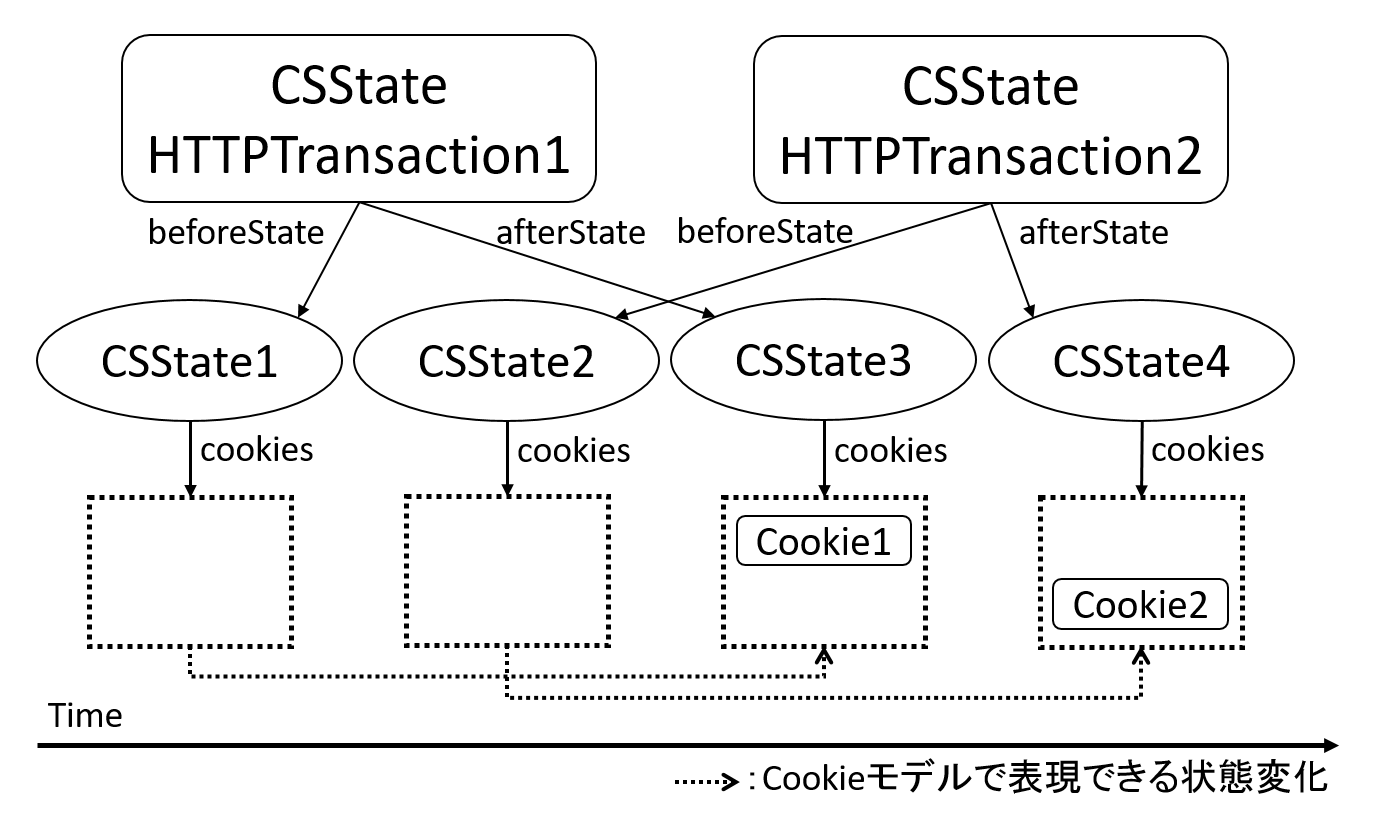
\includegraphics[width=\hsize]{./fig/2transaction-a.eps}
\caption{Cookieモデルで表現可能な状態変化の一例}
\label{fig:2transaction-a}
\end{figure}

\begin{figure}[hbt]
\centering
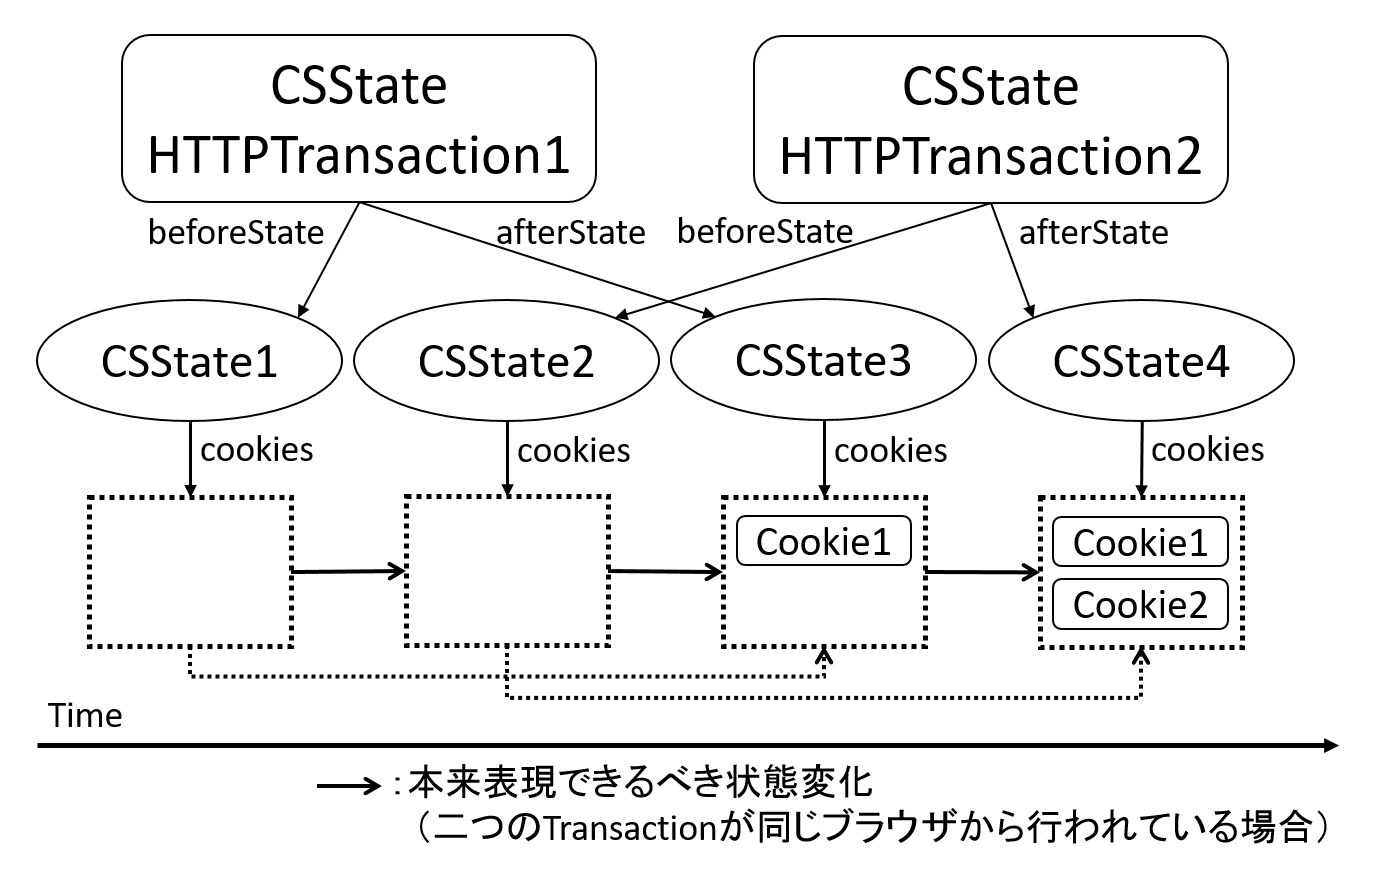
\includegraphics[width=\hsize]{./fig/2transaction-b.eps}
\caption{Cookieモデルで表現不可能な状態変化の一例}
\label{fig:2transaction-b}
\end{figure}

\end{document}

%\documentclass[journal]{IEEEtran}
\usepackage[dvipdfmx]{graphicx}
\usepackage{ascmac}
\usepackage{docmute}
\usepackage{comment}
\usepackage{listings}
\usepackage{listings}
\lstset{
	%枠外での自動改行
 	breaklines = true,
 	%標準の書体
 	%basicstyle = {\small},
 	%枠 "t"は上に線を記載, "T"は上に二重線を記載
	%他オプション:leftline,topline,bottomline,lines,single,shadowbox
 	frame = TB,
 	%タブの大きさ
 	tabsize = 2,
 	%キャプションの場所("tb"ならば上下両方に記載)
 	%captionpos = t,
 	%行番号の位置
 	%numbers = left,
 	%自動改行後のインデント量(デフォルトでは20[pt])	
 	breakindent = 30pt,
	%左右の位置調整 	
 	xleftmargin=15pt,
 	xrightmargin=10pt,
	%プログラム言語(複数の言語に対応,C,C++も可)
 	%language = Python, 	
 	%背景色と透過度
 	%backgroundcolor={\color[gray]{.90}},
 	%コメントの書体
 	%commentstyle = {\itshape \color[cmyk]{1,0.4,1,0}},
 	%関数名等の色の設定
 	%classoffset = 0,
 	%キーワード(int, ifなど)の書体
 	%keywordstyle = {\bfseries \color[cmyk]{0,1,0,0}},
 	%表示する文字の書体
 	%stringstyle = {\ttfamily \color[rgb]{0,0,1}},
 	%frameまでの間隔(行番号とプログラムの間)
 	%framesep = 5pt,
 	%行番号の間隔
 	%stepnumber = 1,
	%行番号の書体
 	%numberstyle = \tiny,
}
\makeatletter
\def\lst@makecaption{%
  \def\@captype{table}%
  \@makecaption
}
\makeatother
\renewcommand{\lstlistingname}{Code}

% Some very useful LaTeX packages include:
% (uncomment the ones you want to load)


% *** MISC UTILITY PACKAGES ***
%
%\usepackage{ifpdf}
% Heiko Oberdiek's ifpdf.sty is very useful if you need conditional
% compilation based on whether the output is pdf or dvi.
% usage:
% \ifpdf
%   % pdf code
% \else
%   % dvi code
% \fi
% The latest version of ifpdf.sty can be obtained from:
% http://www.ctan.org/pkg/ifpdf
% Also, note that IEEEtran.cls V1.7 and later provides a builtin
% \ifCLASSINFOpdf conditional that works the same way.
% When switching from latex to pdflatex and vice-versa, the compiler may
% have to be run twice to clear warning/error messages.


% *** CITATION PACKAGES ***
%
\usepackage{cite}
% cite.sty was written by Donald Arseneau
% V1.6 and later of IEEEtran pre-defines the format of the cite.sty package
% \cite{} output to follow that of the IEEE. Loading the cite package will
% result in citation numbers being automatically sorted and properly
% "compressed/ranged". e.g., [1], [9], [2], [7], [5], [6] without using
% cite.sty will become [1], [2], [5]--[7], [9] using cite.sty. cite.sty's
% \cite will automatically add leading space, if needed. Use cite.sty's
% noadjust option (cite.sty V3.8 and later) if you want to turn this off
% such as if a citation ever needs to be enclosed in parenthesis.
% cite.sty is already installed on most LaTeX systems. Be sure and use
% version 5.0 (2009-03-20) and later if using hyperref.sty.
% The latest version can be obtained at:
% http://www.ctan.org/pkg/cite
% The documentation is contained in the cite.sty file itself.


% *** GRAPHICS RELATED PACKAGES ***
%
\ifCLASSINFOpdf
  % \usepackage[pdftex]{graphicx}
  % declare the path(s) where your graphic files are
  % \graphicspath{{../pdf/}{../jpeg/}}
  % and their extensions so you won't have to specify these with
  % every instance of \includegraphics
  % \DeclareGraphicsExtensions{.pdf,.jpeg,.png}
\else
  % or other class option (dvipsone, dvipdf, if not using dvips). graphicx
  % will default to the driver specified in the system graphics.cfg if no
  % driver is specified.
  % \usepackage[dvips]{graphicx}
  % declare the path(s) where your graphic files are
  % \graphicspath{{../eps/}}
  % and their extensions so you won't have to specify these with
  % every instance of \includegraphics
  % \DeclareGraphicsExtensions{.eps}
\fi
% graphicx was written by David Carlisle and Sebastian Rahtz. It is
% required if you want graphics, photos, etc. graphicx.sty is already
% installed on most LaTeX systems. The latest version and documentation
% can be obtained at: 
% http://www.ctan.org/pkg/graphicx
% Another good source of documentation is "Using Imported Graphics in
% LaTeX2e" by Keith Reckdahl which can be found at:
% http://www.ctan.org/pkg/epslatex
%
% latex, and pdflatex in dvi mode, support graphics in encapsulated
% postscript (.eps) format. pdflatex in pdf mode supports graphics
% in .pdf, .jpeg, .png and .mps (metapost) formats. Users should ensure
% that all non-photo figures use a vector format (.eps, .pdf, .mps) and
% not a bitmapped formats (.jpeg, .png). The IEEE frowns on bitmapped formats
% which can result in "jaggedy"/blurry rendering of lines and letters as
% well as large increases in file sizes.
%
% You can find documentation about the pdfTeX application at:
% http://www.tug.org/applications/pdftex


% *** MATH PACKAGES ***
%
%\usepackage{amsmath}
% A popular package from the American Mathematical Society that provides
% many useful and powerful commands for dealing with mathematics.
%
% Note that the amsmath package sets \interdisplaylinepenalty to 10000
% thus preventing page breaks from occurring within multiline equations. Use:
%\interdisplaylinepenalty=2500
% after loading amsmath to restore such page breaks as IEEEtran.cls normally
% does. amsmath.sty is already installed on most LaTeX systems. The latest
% version and documentation can be obtained at:
% http://www.ctan.org/pkg/amsmath


% *** SPECIALIZED LIST PACKAGES ***
%
%\usepackage{algorithmic}
% algorithmic.sty was written by Peter Williams and Rogerio Brito.
% This package provides an algorithmic environment fo describing algorithms.
% You can use the algorithmic environment in-text or within a figure
% environment to provide for a floating algorithm. Do NOT use the algorithm
% floating environment provided by algorithm.sty (by the same authors) or
% algorithm2e.sty (by Christophe Fiorio) as the IEEE does not use dedicated
% algorithm float types and packages that provide these will not provide
% correct IEEE style captions. The latest version and documentation of
% algorithmic.sty can be obtained at:
% http://www.ctan.org/pkg/algorithms
% Also of interest may be the (relatively newer and more customizable)
% algorithmicx.sty package by Szasz Janos:
% http://www.ctan.org/pkg/algorithmicx


% *** ALIGNMENT PACKAGES ***
%
%\usepackage{array}
% Frank Mittelbach's and David Carlisle's array.sty patches and improves
% the standard LaTeX2e array and tabular environments to provide better
% appearance and additional user controls. As the default LaTeX2e table
% generation code is lacking to the point of almost being broken with
% respect to the quality of the end results, all users are strongly
% advised to use an enhanced (at the very least that provided by array.sty)
% set of table tools. array.sty is already installed on most systems. The
% latest version and documentation can be obtained at:
% http://www.ctan.org/pkg/array


% IEEEtran contains the IEEEeqnarray family of commands that can be used to
% generate multiline equations as well as matrices, tables, etc., of high
% quality.


% *** SUBFIGURE PACKAGES ***
%\ifCLASSOPTIONcompsoc
%  \usepackage[caption=false,font=normalsize,labelfont=sf,textfont=sf]{subfig}
%\else
%  \usepackage[caption=false,font=footnotesize]{subfig}
%\fi
% subfig.sty, written by Steven Douglas Cochran, is the modern replacement
% for subfigure.sty, the latter of which is no longer maintained and is
% incompatible with some LaTeX packages including fixltx2e. However,
% subfig.sty requires and automatically loads Axel Sommerfeldt's caption.sty
% which will override IEEEtran.cls' handling of captions and this will result
% in non-IEEE style figure/table captions. To prevent this problem, be sure
% and invoke subfig.sty's "caption=false" package option (available since
% subfig.sty version 1.3, 2005/06/28) as this is will preserve IEEEtran.cls
% handling of captions.
% Note that the Computer Society format requires a larger sans serif font
% than the serif footnote size font used in traditional IEEE formatting
% and thus the need to invoke different subfig.sty package options depending
% on whether compsoc mode has been enabled.
%
% The latest version and documentation of subfig.sty can be obtained at:
% http://www.ctan.org/pkg/subfig


% *** FLOAT PACKAGES ***
%
%\usepackage{fixltx2e}
% fixltx2e, the successor to the earlier fix2col.sty, was written by
% Frank Mittelbach and David Carlisle. This package corrects a few problems
% in the LaTeX2e kernel, the most notable of which is that in current
% LaTeX2e releases, the ordering of single and double column floats is not
% guaranteed to be preserved. Thus, an unpatched LaTeX2e can allow a
% single column figure to be placed prior to an earlier double column
% figure.
% Be aware that LaTeX2e kernels dated 2015 and later have fixltx2e.sty's
% corrections already built into the system in which case a warning will
% be issued if an attempt is made to load fixltx2e.sty as it is no longer
% needed.
% The latest version and documentation can be found at:
% http://www.ctan.org/pkg/fixltx2e


%\usepackage{stfloats}
% stfloats.sty was written by Sigitas Tolusis. This package gives LaTeX2e
% the ability to do double column floats at the bottom of the page as well
% as the top. (e.g., "\begin{figure*}[!b]" is not normally possible in
% LaTeX2e). It also provides a command:
%\fnbelowfloat
% to enable the placement of footnotes below bottom floats (the standard
% LaTeX2e kernel puts them above bottom floats). This is an invasive package
% which rewrites many portions of the LaTeX2e float routines. It may not work
% with other packages that modify the LaTeX2e float routines. The latest
% version and documentation can be obtained at:
% http://www.ctan.org/pkg/stfloats
% Do not use the stfloats baselinefloat ability as the IEEE does not allow
% \baselineskip to stretch. Authors submitting work to the IEEE should note
% that the IEEE rarely uses double column equations and that authors should try
% to avoid such use. Do not be tempted to use the cuted.sty or midfloat.sty
% packages (also by Sigitas Tolusis) as the IEEE does not format its papers in
% such ways.
% Do not attempt to use stfloats with fixltx2e as they are incompatible.
% Instead, use Morten Hogholm'a dblfloatfix which combines the features
% of both fixltx2e and stfloats:
%
% \usepackage{dblfloatfix}
% The latest version can be found at:
% http://www.ctan.org/pkg/dblfloatfix


%\ifCLASSOPTIONcaptionsoff
%  \usepackage[nomarkers]{endfloat}
% \let\MYoriglatexcaption\caption
% \renewcommand{\caption}[2][\relax]{\MYoriglatexcaption[#2]{#2}}
%\fi
% endfloat.sty was written by James Darrell McCauley, Jeff Goldberg and 
% Axel Sommerfeldt. This package may be useful when used in conjunction with 
% IEEEtran.cls'  captionsoff option. Some IEEE journals/societies require that
% submissions have lists of figures/tables at the end of the paper and that
% figures/tables without any captions are placed on a page by themselves at
% the end of the document. If needed, the draftcls IEEEtran class option or
% \CLASSINPUTbaselinestretch interface can be used to increase the line
% spacing as well. Be sure and use the nomarkers option of endfloat to
% prevent endfloat from "marking" where the figures would have been placed
% in the text. The two hack lines of code above are a slight modification of
% that suggested by in the endfloat docs (section 8.4.1) to ensure that
% the full captions always appear in the list of figures/tables - even if
% the user used the short optional argument of \caption[]{}.
% IEEE papers do not typically make use of \caption[]'s optional argument,
% so this should not be an issue. A similar trick can be used to disable
% captions of packages such as subfig.sty that lack options to turn off
% the subcaptions:
% For subfig.sty:
% \let\MYorigsubfloat\subfloat
% \renewcommand{\subfloat}[2][\relax]{\MYorigsubfloat[]{#2}}
% However, the above trick will not work if both optional arguments of
% the \subfloat command are used. Furthermore, there needs to be a
% description of each subfigure *somewhere* and endfloat does not add
% subfigure captions to its list of figures. Thus, the best approach is to
% avoid the use of subfigure captions (many IEEE journals avoid them anyway)
% and instead reference/explain all the subfigures within the main caption.
% The latest version of endfloat.sty and its documentation can obtained at:
% http://www.ctan.org/pkg/endfloat
%
% The IEEEtran \ifCLASSOPTIONcaptionsoff conditional can also be used
% later in the document, say, to conditionally put the References on a 
% page by themselves.


% *** PDF, URL AND HYPERLINK PACKAGES ***
%
%\usepackage{url}
% url.sty was written by Donald Arseneau. It provides better support for
% handling and breaking URLs. url.sty is already installed on most LaTeX
% systems. The latest version and documentation can be obtained at:
% http://www.ctan.org/pkg/url
% Basically, \url{my_url_here}.

\begin{document}

\section{Alloyにおける時相論理の記述法の提案}
\label{sec:ProposedModel-TemporalLogic}
この章では、イベント発生時におけるウェブの様々な要素の状態変化の表現に利用可能なAlloyでの時相論理の記述法を提案する。

前述の\ref{sec:existing-models-problems}節における既存モデルの時相論理の表現能力の主な問題点は、「3状態以上の遷移を表現できない」ことである。
この問題は、Cookieモデルにおいて状態クラス(CookieモデルにけるCSStateクラス)間の関係性がHTTPTransactionクラスのみを用いて表現されていることに起因している。
この方式では同一のHTTPTransacion内の状態変化しか表現できない。
したがって、HTTPTransactionクラスに依存せずに、状態クラス間の関係性を表現する方式が必要となる。
また、CookieモデルにおけるCSStateはCookieの状態を表現するクラスであり、ウェブの他の要素を表現するための拡張性に乏しい。
そこで、拡張性を高めるため、様々なウェブの構成要素の状態を表現するための汎用的な状態クラスを定義し、その状態クラス間の関係性を表現することを目標とする。

本研究では各状態クラス間の状態遷移の表現のために必要な命題論理を、述語として容易に利用できる形式にまとめる。
ここで、時間軸全体を通した状態遷移を表現するためにどのような述語が必要となるかを考える。
まず、ある二状態に対してそれらが時間軸上で連続しているかを判定できれば、
「前後の二状態で起こりうる変化」を表現可能になる。
これに加えて状態遷移の初期状態を判定できれば、「初期状態にかかる条件(初期条件)」を表現可能になる。
これら二つの表現能力を組み合わせることで、帰納的に時間軸全体で起こりうる状態変化を表現可能となる。
以上より、時間軸全体での状態変化を表現するために以下の述語を作成する。
\begin{itemize}
\item 状態遷移において、直前にあたる状態を判定する述語
\item 初期状態を判定する述語
\end{itemize}

また、本記述法を用いる上で基礎モデルでの時間軸の表現(\ref{sec:based-model}節参照)を一部変更している。
その変更点については\ref{sec:TimeClass}節で述べる。

\subsection{時間軸の表現の変更}
\label{sec:TimeClass}
基礎モデル\cite{based-model}においては、時間軸を表すTimeクラスにネットワーク上で発生するレスポンスやリクエストを表すEventクラスが関連付けられている。
これらのクラス間の関係性は、「ある時点Time0とTime1の間でEvent0が発生した」といった内容を表現できるものであり、二つのTimeクラスのインスタンスで一つのイベントの時刻を表現できる。
この関係性はEventのみが時間軸に関連付けられていたために利用できた。

これに対し、本提案記述法ではEventクラスに加えて、ある時点におけるウェブの要素の状態を表すStateクラスも時間軸に関連付けられる。
ここで、二つのTimeクラスのインスタンスで一つのイベントの時刻を表現するという既存モデルの関係性を維持すると、導入する述語の論理式が複雑となり実装が困難となる。
したがって、本提案モデルでは図\ref{fig:ProposedModel-TimeClass}に示す、一つのTimeクラスのインスタンスでイベントの時刻を表現できる記述法に変更する。

\begin{figure}[htb]
\centering
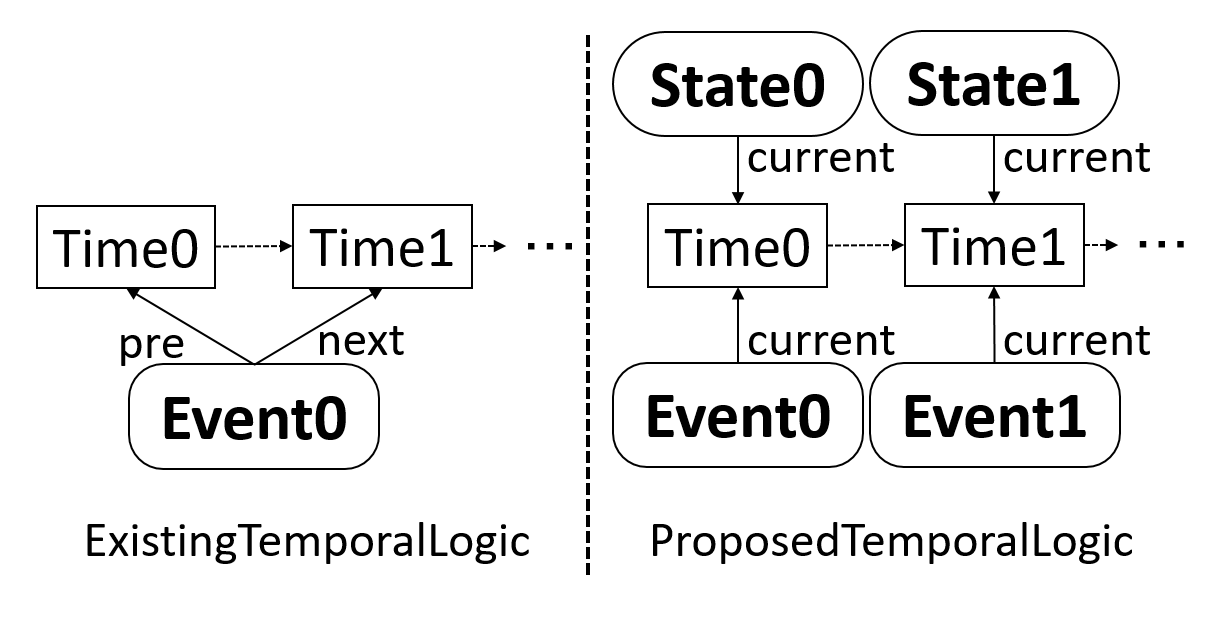
\includegraphics[width=\hsize]{./fig/TimeClass.eps}
\caption{提案モデルにおける時間軸とイベントの関係}
\label{fig:TimeClass}
\end{figure}

この表現の変更によって、二つの既存モデルそれぞれにおける時相論理の表現能力に変更はない。
そもそも基礎モデルにおいて、二つのTimeクラスのインスタンスを利用する関係性を採用した理由は今後の拡張性を想定したためである。
基礎モデルには「リクエストやレスポンスといったイベントが同時刻で発生しない」といった制限が存在しており、このようなTimeクラスの関係性を用いていた場合には、この制限を取り払う拡張が容易となると考えられていた。
しかし、表現の変更後も同様に制限を取り除く拡張は可能である。
つまり、この変更によって既存モデルの表現能力と拡張性を妨げることはない。

\subsection{汎用的な状態クラス}
\label{sec:state-class}
導入する状態クラスとしてCode\ref{code:StateClass}に示すStateクラスを定義する。
このStateクラスの要素であるflowはStateクラス同士を接続し状態の遷移を表し、currentはその状態となり得る時刻を表す。
また、その他の項目としてEqItem、DifItemクラスをStateクラスの変数としている。
\begin{lstlisting}[caption=Stateクラス, label=code:StateClass]
abstract sig State{
	flow: set State,
	eq: one EqItem,
	dif: one DifItem,
	current: set Time
}
abstract sig EqItem{}
abstract sig DifItem{}
sig StateTransaction extends HTTPTransaction{
	beforeState: set State,
	afterState: set State
}
\end{lstlisting}

まず、EqItemは同一の状態遷移上で変化しない要素(以下、「不変項目」とする)を表すクラスである。
不変項目は複数のStateが存在する場合に、いずれのStateが同一の遷移であるのかを判定するために用いる。
これは、ウェブ上には様々な要素が存在し、それらの要素が各一つずつであるとは限らないためである。
このような場合には、状態遷移が並列に混在するため、どのインスタンスが同一の遷移に属するかを判定する必要があり、不変項目はこれを可能とする。

また、DifItemは状態遷移において変化する要素(以下、「変化項目」とする)を表すクラスである。
この部分には、あるウェブの要素の状態変化を表現する上で変化しうる内容を記述する。

最後に、これらのStateはCookieモデルと同様にHTTPTransactionに関連付けることで、レスポンスとリクエスト時の状態を表すように配置する。
具体的に、HTTPTransactionを継承しStateクラスを持つStateTransactionをCode\ref{code:StateClass}の9-12行目で定義している。

このStateクラスを利用してウェブの要素の状態遷移を考えるには、State、EqItem、DifItemクラスを継承するその要素専用のクラスを定義する。
また、その要素について不変項目と変化項目を明らかにしておき、継承後のクラスに記述する。
以下のCode\ref{code:CookieClass}はCookieモデルを基にしたCookieへの応用例である。
2,3行目に記すように、Stateを継承するクラスではeqとdifもまた、EqItem、DifItemを継承する専用のクラスに含まれるように条件を記述する。
Cookieモデルでは、不変項目がクライアント、変化項目がCookieの集合となっている。
これは、各クライアント毎にCookieの保存が行われているため、状態遷移の上でクライアントは変更されないためである。
また、変化項目は状態遷移で変化しうる要素、つまり、クライアント内で保存されているCookieを表現する。
\begin{lstlisting}[caption=Cookieへの応用例, label=code:CookieClass]
sig CookieState extends State{}{
	eq in CookieEqItem
	dif in CookieDifItem
}
sig CookieEqItem extends EqItem{
	client: one HTTPClient
}
sig CookieDifItem extends DifItem{
	cookie: set Cookie
}
\end{lstlisting}

\subsection{直前の状態を判定する述語}
\ref{sec:state-class}で述べたStateクラスに対して、同一の状態遷移上で直前となる状態を判定する述語LastStateを利用できる。
このLastStateは三つの引数を要し、そのうちの二つはStateでありそれぞれpre、postと表す。
ここで、述語LastStateはpreがpostの直前の状態である場合に真となるよう作成する。
しかし、postが複数の時刻で継続している状態である場合にはpostは複数の時刻を持つ。
したがって、この二つの入力のみでは一つのpostに対して真となるpreが複数存在することになる。
これを防ぐために、postの時刻を指定するStateTransactionを引数に追加する(これをstrとする)。
これにより、与えられたトランザクションに含まれるpostの時刻に限定して、その時刻においてpreが直前であるか判定でき、真となる組み合わせが一意に定まる。
このように作成した述語LastStateをCode\ref{code:LastState}に示す。

\begin{lstlisting}[caption=状態遷移において直前の状態を判定する述語, label=code:LastState]
pred LastState[pre:State, post:State, str:StateTransaction]{
	pre.eq = post.eq
	post in str.(beforeState + afterState)

	some t,t':Time |
		{
			t in pre.current
			t' in str.(request + response + re_res).current
			t' in str.request.current implies post in str.beforeState
			t' in str.(response + re_res).current implies post in str.afterState
			t' in t.next.*next

			all s:State, t'':Time |
				(s.eq = pre.eq and t'' in s.current) implies
						(t in t''.*next) or (t'' in t'.*next)
		}
}
\end{lstlisting}

また、述語LastStateが真となる条件は以下のように整理できる。
\begin{itembox}[l]{LastState}
LastStateは引数pre,post(Stateクラス), str(StateTransactionクラス)が以下をすべて満たす場合に真となる。
\begin{itemize}
\item preとpostの不変項目が同一である
\item postがstrのbeforeState、afterStateのいずれかに属している
\item preの時刻とpostのstrにおける時刻の間の時刻を持つ、不変項目が同一の他の状態が存在しない
\end{itemize}
\end{itembox}

\subsection{初期状態を判定する述語}
Stateクラスに対して利用可能な、もう一方の述語は初期状態を判定する述語InitialStateである(Code\ref{code:InitialState}参照)。
引数としてStateクラスが与えられ(これをsとする)、それが初期状態であるか判定する。
また、不変項目が異なると状態変化がそれぞれ独立するため、それぞれに対して初期状態が生じる(図\ref{fig:InitialState})。
\begin{lstlisting}[caption=状態遷移において初期状態を判定する述語, label=code:InitialState]
pred InitialState[s:State]{
	all s':State |
		s.eq = s'.eq implies
			s'.current in s.current.*next
}
\end{lstlisting}

\begin{itembox}[l]{InitialState}
InitialStateは引数s(Stateクラス)に対して、sと同じ不変要素を持つStateクラスのインスタンスがすべてsの時刻以降の状態である場合に真となる
\end{itembox}

\end{document}

%\documentclass[journal]{IEEEtran}
\usepackage[dvipdfmx]{graphicx}
\usepackage{ascmac}
\usepackage{docmute}
\usepackage{comment}
\usepackage{listings}
\usepackage{listings}
\lstset{
	%枠外での自動改行
 	breaklines = true,
 	%標準の書体
 	%basicstyle = {\small},
 	%枠 "t"は上に線を記載, "T"は上に二重線を記載
	%他オプション:leftline,topline,bottomline,lines,single,shadowbox
 	frame = TB,
 	%タブの大きさ
 	tabsize = 2,
 	%キャプションの場所("tb"ならば上下両方に記載)
 	%captionpos = t,
 	%行番号の位置
 	%numbers = left,
 	%自動改行後のインデント量(デフォルトでは20[pt])	
 	breakindent = 30pt,
	%左右の位置調整 	
 	xleftmargin=15pt,
 	xrightmargin=10pt,
	%プログラム言語(複数の言語に対応,C,C++も可)
 	%language = Python, 	
 	%背景色と透過度
 	%backgroundcolor={\color[gray]{.90}},
 	%コメントの書体
 	%commentstyle = {\itshape \color[cmyk]{1,0.4,1,0}},
 	%関数名等の色の設定
 	%classoffset = 0,
 	%キーワード(int, ifなど)の書体
 	%keywordstyle = {\bfseries \color[cmyk]{0,1,0,0}},
 	%表示する文字の書体
 	%stringstyle = {\ttfamily \color[rgb]{0,0,1}},
 	%frameまでの間隔(行番号とプログラムの間)
 	%framesep = 5pt,
 	%行番号の間隔
 	%stepnumber = 1,
	%行番号の書体
 	%numberstyle = \tiny,
}
\makeatletter
\def\lst@makecaption{%
  \def\@captype{table}%
  \@makecaption
}
\makeatother
\renewcommand{\lstlistingname}{Code}

% Some very useful LaTeX packages include:
% (uncomment the ones you want to load)


% *** MISC UTILITY PACKAGES ***
%
%\usepackage{ifpdf}
% Heiko Oberdiek's ifpdf.sty is very useful if you need conditional
% compilation based on whether the output is pdf or dvi.
% usage:
% \ifpdf
%   % pdf code
% \else
%   % dvi code
% \fi
% The latest version of ifpdf.sty can be obtained from:
% http://www.ctan.org/pkg/ifpdf
% Also, note that IEEEtran.cls V1.7 and later provides a builtin
% \ifCLASSINFOpdf conditional that works the same way.
% When switching from latex to pdflatex and vice-versa, the compiler may
% have to be run twice to clear warning/error messages.


% *** CITATION PACKAGES ***
%
\usepackage{cite}
% cite.sty was written by Donald Arseneau
% V1.6 and later of IEEEtran pre-defines the format of the cite.sty package
% \cite{} output to follow that of the IEEE. Loading the cite package will
% result in citation numbers being automatically sorted and properly
% "compressed/ranged". e.g., [1], [9], [2], [7], [5], [6] without using
% cite.sty will become [1], [2], [5]--[7], [9] using cite.sty. cite.sty's
% \cite will automatically add leading space, if needed. Use cite.sty's
% noadjust option (cite.sty V3.8 and later) if you want to turn this off
% such as if a citation ever needs to be enclosed in parenthesis.
% cite.sty is already installed on most LaTeX systems. Be sure and use
% version 5.0 (2009-03-20) and later if using hyperref.sty.
% The latest version can be obtained at:
% http://www.ctan.org/pkg/cite
% The documentation is contained in the cite.sty file itself.


% *** GRAPHICS RELATED PACKAGES ***
%
\ifCLASSINFOpdf
  % \usepackage[pdftex]{graphicx}
  % declare the path(s) where your graphic files are
  % \graphicspath{{../pdf/}{../jpeg/}}
  % and their extensions so you won't have to specify these with
  % every instance of \includegraphics
  % \DeclareGraphicsExtensions{.pdf,.jpeg,.png}
\else
  % or other class option (dvipsone, dvipdf, if not using dvips). graphicx
  % will default to the driver specified in the system graphics.cfg if no
  % driver is specified.
  % \usepackage[dvips]{graphicx}
  % declare the path(s) where your graphic files are
  % \graphicspath{{../eps/}}
  % and their extensions so you won't have to specify these with
  % every instance of \includegraphics
  % \DeclareGraphicsExtensions{.eps}
\fi
% graphicx was written by David Carlisle and Sebastian Rahtz. It is
% required if you want graphics, photos, etc. graphicx.sty is already
% installed on most LaTeX systems. The latest version and documentation
% can be obtained at: 
% http://www.ctan.org/pkg/graphicx
% Another good source of documentation is "Using Imported Graphics in
% LaTeX2e" by Keith Reckdahl which can be found at:
% http://www.ctan.org/pkg/epslatex
%
% latex, and pdflatex in dvi mode, support graphics in encapsulated
% postscript (.eps) format. pdflatex in pdf mode supports graphics
% in .pdf, .jpeg, .png and .mps (metapost) formats. Users should ensure
% that all non-photo figures use a vector format (.eps, .pdf, .mps) and
% not a bitmapped formats (.jpeg, .png). The IEEE frowns on bitmapped formats
% which can result in "jaggedy"/blurry rendering of lines and letters as
% well as large increases in file sizes.
%
% You can find documentation about the pdfTeX application at:
% http://www.tug.org/applications/pdftex


% *** MATH PACKAGES ***
%
%\usepackage{amsmath}
% A popular package from the American Mathematical Society that provides
% many useful and powerful commands for dealing with mathematics.
%
% Note that the amsmath package sets \interdisplaylinepenalty to 10000
% thus preventing page breaks from occurring within multiline equations. Use:
%\interdisplaylinepenalty=2500
% after loading amsmath to restore such page breaks as IEEEtran.cls normally
% does. amsmath.sty is already installed on most LaTeX systems. The latest
% version and documentation can be obtained at:
% http://www.ctan.org/pkg/amsmath


% *** SPECIALIZED LIST PACKAGES ***
%
%\usepackage{algorithmic}
% algorithmic.sty was written by Peter Williams and Rogerio Brito.
% This package provides an algorithmic environment fo describing algorithms.
% You can use the algorithmic environment in-text or within a figure
% environment to provide for a floating algorithm. Do NOT use the algorithm
% floating environment provided by algorithm.sty (by the same authors) or
% algorithm2e.sty (by Christophe Fiorio) as the IEEE does not use dedicated
% algorithm float types and packages that provide these will not provide
% correct IEEE style captions. The latest version and documentation of
% algorithmic.sty can be obtained at:
% http://www.ctan.org/pkg/algorithms
% Also of interest may be the (relatively newer and more customizable)
% algorithmicx.sty package by Szasz Janos:
% http://www.ctan.org/pkg/algorithmicx


% *** ALIGNMENT PACKAGES ***
%
%\usepackage{array}
% Frank Mittelbach's and David Carlisle's array.sty patches and improves
% the standard LaTeX2e array and tabular environments to provide better
% appearance and additional user controls. As the default LaTeX2e table
% generation code is lacking to the point of almost being broken with
% respect to the quality of the end results, all users are strongly
% advised to use an enhanced (at the very least that provided by array.sty)
% set of table tools. array.sty is already installed on most systems. The
% latest version and documentation can be obtained at:
% http://www.ctan.org/pkg/array


% IEEEtran contains the IEEEeqnarray family of commands that can be used to
% generate multiline equations as well as matrices, tables, etc., of high
% quality.


% *** SUBFIGURE PACKAGES ***
%\ifCLASSOPTIONcompsoc
%  \usepackage[caption=false,font=normalsize,labelfont=sf,textfont=sf]{subfig}
%\else
%  \usepackage[caption=false,font=footnotesize]{subfig}
%\fi
% subfig.sty, written by Steven Douglas Cochran, is the modern replacement
% for subfigure.sty, the latter of which is no longer maintained and is
% incompatible with some LaTeX packages including fixltx2e. However,
% subfig.sty requires and automatically loads Axel Sommerfeldt's caption.sty
% which will override IEEEtran.cls' handling of captions and this will result
% in non-IEEE style figure/table captions. To prevent this problem, be sure
% and invoke subfig.sty's "caption=false" package option (available since
% subfig.sty version 1.3, 2005/06/28) as this is will preserve IEEEtran.cls
% handling of captions.
% Note that the Computer Society format requires a larger sans serif font
% than the serif footnote size font used in traditional IEEE formatting
% and thus the need to invoke different subfig.sty package options depending
% on whether compsoc mode has been enabled.
%
% The latest version and documentation of subfig.sty can be obtained at:
% http://www.ctan.org/pkg/subfig


% *** FLOAT PACKAGES ***
%
%\usepackage{fixltx2e}
% fixltx2e, the successor to the earlier fix2col.sty, was written by
% Frank Mittelbach and David Carlisle. This package corrects a few problems
% in the LaTeX2e kernel, the most notable of which is that in current
% LaTeX2e releases, the ordering of single and double column floats is not
% guaranteed to be preserved. Thus, an unpatched LaTeX2e can allow a
% single column figure to be placed prior to an earlier double column
% figure.
% Be aware that LaTeX2e kernels dated 2015 and later have fixltx2e.sty's
% corrections already built into the system in which case a warning will
% be issued if an attempt is made to load fixltx2e.sty as it is no longer
% needed.
% The latest version and documentation can be found at:
% http://www.ctan.org/pkg/fixltx2e


%\usepackage{stfloats}
% stfloats.sty was written by Sigitas Tolusis. This package gives LaTeX2e
% the ability to do double column floats at the bottom of the page as well
% as the top. (e.g., "\begin{figure*}[!b]" is not normally possible in
% LaTeX2e). It also provides a command:
%\fnbelowfloat
% to enable the placement of footnotes below bottom floats (the standard
% LaTeX2e kernel puts them above bottom floats). This is an invasive package
% which rewrites many portions of the LaTeX2e float routines. It may not work
% with other packages that modify the LaTeX2e float routines. The latest
% version and documentation can be obtained at:
% http://www.ctan.org/pkg/stfloats
% Do not use the stfloats baselinefloat ability as the IEEE does not allow
% \baselineskip to stretch. Authors submitting work to the IEEE should note
% that the IEEE rarely uses double column equations and that authors should try
% to avoid such use. Do not be tempted to use the cuted.sty or midfloat.sty
% packages (also by Sigitas Tolusis) as the IEEE does not format its papers in
% such ways.
% Do not attempt to use stfloats with fixltx2e as they are incompatible.
% Instead, use Morten Hogholm'a dblfloatfix which combines the features
% of both fixltx2e and stfloats:
%
% \usepackage{dblfloatfix}
% The latest version can be found at:
% http://www.ctan.org/pkg/dblfloatfix


%\ifCLASSOPTIONcaptionsoff
%  \usepackage[nomarkers]{endfloat}
% \let\MYoriglatexcaption\caption
% \renewcommand{\caption}[2][\relax]{\MYoriglatexcaption[#2]{#2}}
%\fi
% endfloat.sty was written by James Darrell McCauley, Jeff Goldberg and 
% Axel Sommerfeldt. This package may be useful when used in conjunction with 
% IEEEtran.cls'  captionsoff option. Some IEEE journals/societies require that
% submissions have lists of figures/tables at the end of the paper and that
% figures/tables without any captions are placed on a page by themselves at
% the end of the document. If needed, the draftcls IEEEtran class option or
% \CLASSINPUTbaselinestretch interface can be used to increase the line
% spacing as well. Be sure and use the nomarkers option of endfloat to
% prevent endfloat from "marking" where the figures would have been placed
% in the text. The two hack lines of code above are a slight modification of
% that suggested by in the endfloat docs (section 8.4.1) to ensure that
% the full captions always appear in the list of figures/tables - even if
% the user used the short optional argument of \caption[]{}.
% IEEE papers do not typically make use of \caption[]'s optional argument,
% so this should not be an issue. A similar trick can be used to disable
% captions of packages such as subfig.sty that lack options to turn off
% the subcaptions:
% For subfig.sty:
% \let\MYorigsubfloat\subfloat
% \renewcommand{\subfloat}[2][\relax]{\MYorigsubfloat[]{#2}}
% However, the above trick will not work if both optional arguments of
% the \subfloat command are used. Furthermore, there needs to be a
% description of each subfigure *somewhere* and endfloat does not add
% subfigure captions to its list of figures. Thus, the best approach is to
% avoid the use of subfigure captions (many IEEE journals avoid them anyway)
% and instead reference/explain all the subfigures within the main caption.
% The latest version of endfloat.sty and its documentation can obtained at:
% http://www.ctan.org/pkg/endfloat
%
% The IEEEtran \ifCLASSOPTIONcaptionsoff conditional can also be used
% later in the document, say, to conditionally put the References on a 
% page by themselves.


% *** PDF, URL AND HYPERLINK PACKAGES ***
%
%\usepackage{url}
% url.sty was written by Donald Arseneau. It provides better support for
% handling and breaking URLs. url.sty is already installed on most LaTeX
% systems. The latest version and documentation can be obtained at:
% http://www.ctan.org/pkg/url
% Basically, \url{my_url_here}.

\begin{document}

\section{提案モデル}
この章では、\ref{sec:ProposedModel-TemporalLogic}章で述べた記述法の応用例として、キャッシュを実装したウェブセキュリティモデルを提案する。

本研究では基礎モデルで包括されていないウェブの要素としてキャッシュに注目する。
\ref{sec:introduction}章に述べた通りキャッシュを利用する攻撃が数多く存在しており、また、キャッシュは一般的なユーザにも利用されるウェブの構成要素である。
したがって、キャッシュに関連した脆弱性はウェブの利用者に多大な影響を与えるため、ウェブの安全性を解析する上で不可欠な要素である。

\subsection{提案モデルの包括内容}
\label{sec:ProposedModel-Content}
提案モデルは基礎モデルを基に作成する。
基礎モデルからの変更点を以下に述べる。

\subsubsection{キャッシュ}
キャッシュはクライアント、サーバ、中継者のいずれかに属し、「格納と削除」、「再利用」、「検証」という三つの基本動作が可能である。
また、これらのキャッシュの動作はヘッダによって制御される。

\subsubsection{中継者}
中継者はクライアントやサーバとは異なるHTTPを構成する第三の要素であり、クライアントとサーバの通信経路上に存在する。
HTTP/1.1において、中継者は「プロキシ」、「ゲートウェイ」、「トンネル」の三種類が存在するが、これらのうちトンネルのみキャッシュを搭載しない。
したがって、キャッシュに注目する本提案モデルではプロキシとゲートウェイのみを包括する。

まず、中継者は独自にリクエストやレスポンスを生成することはなく、取得したリクエストやレスポンスの回送のみを行う。
しかし、キャッシュを用いた場合にのみ、リクエストをサーバに回送しレスポンスを得ることなく、キャッシュの再利用をもってリクエストに応答することができる。
また、プロキシとゲートウェイはその通信内容の編集が可能である。

\subsubsection{HTTPヘッダ}
基礎モデルに含まれるヘッダではキャッシュの動作の表現に不十分であるため、表\ref{tb:ProposedModel-Headers}に挙げるヘッダを新たに追加する。

\begin{table}[htb]
\centering
\caption{提案モデルで新たに包括するヘッダ}
\label{tb:ProposedModel-Headers}
\begin{tabular}{ll}
\hline
ヘッダ名 & 目的 \\
\hline
if-modified-since & 条件付きリクエストに使用 \\
if-none-match & 条件付きリクエストに使用 \\
etag & レスポンス内のコンテンツの固有値 \\
last-modified & レスポンス内のコンテンツの最終更新日 \\
age & レスポンスの経過時間 \\
cache-control & キャッシュの動作全般を制御 \\
date & レスポンスの生成時刻 \\
expire & レスポンスの有効期限 \\
\hline
\end{tabular}
\end{table}

また、表\ref{tb:ProposedModel-Headers}内のcache-controlヘッダはオプションによってキャッシュの動作を指定するため、そのオプションを付加可能とする。
利用可能なオプションを表\ref{tb:CacheControlOption}に挙げる。

\begin{table}[htb]
\centering
\caption{利用可能なcache-controlヘッダのオプション}
\label{tb:CacheControlOption}
\begin{tabular}{ll}
\hline
オプション名 & 用途 \\
\hline
max-age & レスポンスの有効期限を設定 \\
smax-age & 共有キャッシュでの有効期限を設定(最優先) \\
no-cache & 検証無しに再利用できない \\
no-store & そのレスポンスを格納を禁止 \\
no-transform & コンテンツの編集を禁止 \\
max-stale & 期限切れである場合に許容できる時間 \\
min-fresh & 有効期限まで最低残り時間 \\
only-if-cached & キャッシュの再利用でのみ応答 \\
must-revalidate & 有効期限切れの場合、検証無しに再利用できない \\
proxy-revalidate & must-revalidateと同じ(個人キャッシュ以外) \\
public & 共有キャッシュに格納してよい \\
private & 個人キャッシュに格納してよい \\
\hline
\end{tabular}
\end{table}

これら表\ref{tb:ProposedModel-Headers},\ref{tb:ProposedModel-Headers}の各項目のふるまいはHTTP/1.1の仕様に準拠する。

\subsubsection{ブラウザ}
基礎モデルでは表現の単純化のため、「ブラウザのメモリ領域は書き込みのみ可能」という制限がある。
しかし、この制限下ではキャッシュ内の格納レスポンスの削除や検証といった動作を実行することができず、キャッシュの動作を十分に表現することができない。
本研究で提案する時相論理の記述法を用いることでレスポンスの削除といった動作は容易に表現できるため、提案モデルではこの制限を取り除く。

\subsubsection{脅威モデル}
提案モデルの脅威モデルは基礎モデルのものを継承している。
すなわち、三種類の攻撃者とユーザのふるまいを脅威モデルとして設定し、攻撃者にキャッシュと中継者に関する攻撃の能力を新たに付与する。
以下に、三種類の攻撃者それぞれに付与する能力を示す。

\begin{itemize}
\item Web Attackerは複数の中継者を所有することができる。
しかし、その通信内容の編集や通信の遮断をすることはできず、内容をそのままに回送することのみ可能とする。
ただし、暗号化されていない場合、その通信内容を盗聴することは可能とする。
また、保有するクライアント、サーバ、中継者にキャッシュを搭載し、仕様通りに運用できる。
\item Network Attackerは上記のWeb Attackerの能力を全て持つ。
これに加えて、中継者を用いた暗号化されていない通信内容の改ざんと、通信の遮断は可能とする。
\item Gadget Attackerは中継者とキャッシュに関する能力は上記のNetwork Attackerと同様の能力を持つ。
\end{itemize}

\subsubsection{安全性要件}
基礎モデルには二つの安全性要件が設定されており、これらの変更はない。
ただし、Security Invariantsにおける「ウェブの各構成要素の仕様を侵さない」という文言にキャッシュや中継者の仕様を含む。

\subsection{キャッシュの作成}
\label{sec:CacheClass}
キャッシュを表すクラスをCode\ref{code:CacheClass}のように記述する。
抽象クラスとしてCacheクラスを定義し、個人キャッシュを表すPrivateCacheクラス、共有キャッシュを表すPublicCacheクラスを定義する。
また、CacheクラスにはCode\ref{code:LimitedCacheClass}に記述する制限を付与する。
付与される制限は以下の二点である。
\begin{itemize}
\item どのネットワーク上の端末にも属さないキャッシュは存在しない
\item 個人キャッシュはクライアントに属する
\item 共有キャッシュはサーバ、もしくは中継者に属する
\end{itemize}

\begin{lstlisting}[caption=Cacheクラス, label=code:CacheClass]
abstract sig Cache{}
sig PrivateCache extends Cache{}
sig PublicCache extends Cache{}
\end{lstlisting}

また、キャッシュを搭載するため、Code\ref{code:EndPoint}のように、構成要素のクラスを変更する。
HTTPにおけるクライアント、サーバ、中継者を包括するHTTPConfirmistクラスにCacheクラスを追加する。
また、このとき各端末は多くとも一台のキャッシュしか保有することができないものとする。
\begin{lstlisting}[caption=HTTPを利用するウェブの構成要素, label=code:EndPoint]
abstract sig HTTPConformist extends NetworkEndpoint{
	cache : lone Cache
}
\end{lstlisting}

\subsection{キャッシュの状態を表現するクラス}
\label{sec:CacheState}
Code\ref{code:CacheStateClass}のように、時間軸上の各時点におけるキャッシュの状態を表現するCacheStateクラスを作成する。
このCacheStateクラスはStateクラスを継承し、作成した時相論理に関する述語を利用可能な形式とする。
ここで、Stateクラスで定義した「不変項目」はCode\ref{code:CacheClass}で定義したCacheクラス、「変化項目」は格納レスポンスを表現するためのレスポンスの有限集合とする。
これに従い、不変項目を表すCacheEqItem、変化項目を表すCacheDifItemをCode\ref{code:CacheStateClass}に定義する。

また、Code\ref{code:CacheStateClass}では省略しているが、CacheStateには以下の制限を付与する。
これは、レスポンスがキャッシュに格納される場合に満たされなければならないの条件であり、HTTP/1.1の仕様に従っている。
\begin{itemize}
\item 個人キャッシュに格納されている場合、cache-controlヘッダのmax-ageオプション、もしくはdateヘッダとexpireヘッダが一つ含まれる
\item 共有キャッシュに格納されている場合、cache-controlヘッダのmax-ageオプション、s-maxageオプション、dateヘッダとexpireヘッダのいずれかが一つ含まれる
\item キャッシュに格納されている場合、必ずageヘッダが一つ含まれる
\end{itemize}

\begin{lstlisting}[caption=キャッシュの状態を表すクラス, label=code:CacheStateClass]
sig CacheState extends State{}{
	eq in CacheEqItem
	dif in CacheDifItem

	...
}
sig CacheEqItem extends EqItem{cache: one Cache}
sig CacheDifItem extends DifItem{store: set HTTPResponse}
\end{lstlisting}

また、これらの他に以下の制限を加える。
これらの制限は直接的に解析結果に影響するものではないが、可能な限りインスタンスの数を減らし解析を容易にするための工夫である。

\begin{itemize}
\item 同一内容のStateのインスタンスが複数存在しない。異なる時刻で同じ状態を取る場合には同じStateクラスに統合される
\item キャッシュが搭載されている端末が通信を行った場合に、そのキャッシュの状態が必ずインスタンスとして表現される
\item キャッシュに格納されている場合、必ずageヘッダが一つ含まれる
\end{itemize}

\subsection{キャッシュの動作}
\ref{sec:CacheClass}節で定義したCacheStateクラスを用いて、\ref{sec:ProposedModel-Content}節で述べたキャッシュの基本的な3つの動作をAlloyで表現する。

\subsubsection{レスポンスの格納と削除}
提案モデルにおいて、キャッシュにおけるレスポンスの格納と削除は以下のように動作するものとする。

\begin{itembox}[l]{レスポンスの格納}
キャッシュは、そのキャッシュが存在する端末が送受信したレスポンスを格納できる。
そのタイミングは、格納レスポンスを送受信したタイミングとする。
また、格納レスポンスは格納することのできる条件をすべて満たしているものとする。
\end{itembox}

\begin{itembox}[l]{レスポンスの削除}
キャッシュは任意のタイミングで、格納されているレスポンスをキャッシュ内から削除できる。
\end{itembox}

上記で定めたレスポンスの格納と削除は図\ref{fig:ProposedModel-ResponseStoreDelete}のように、二状態間の状態変化として表現する。
まず、レスポンスの格納はレスポンス時のキャッシュの状態において、格納レスポンスにそのレスポンスを追加することで表現できる。
これは、図\ref{fig:ProposedModel-ResponseStoreDelete}内のCacheState0,1における状態変化にあたる。
CacheState0は変化項目としてCacheDifItem0を持ち、CacheState1はCacheDifItem1を持つ。
そして、CacheDifItem0は格納レスポンスの集合が空集合であり、CacheDifItem1は格納レスポンスの集合にResponse0を持つ。
これは、StateTransaction0におけるレスポンスがResponse0であり、レスポンス時にそれがCache0に格納されたことを表す。
また、レスポンスの削除は前状態における格納レスポンスの一部を次状態に引き継がないことで表現する。
これは、図\ref{fig:ProposedModel-ResponseStoreDelete}内のCacheState1と2における状態変化にあたる。
この場合、CacheState2は変化項目としてCacheDifItem0を持つため、上述の格納の場合と状態変化が逆になる。
つまり、CacheState1の時点でCache0が格納していたResponse0を、CacheState2の時点では削除していることを表している。

\begin{figure}[htb]
\centering
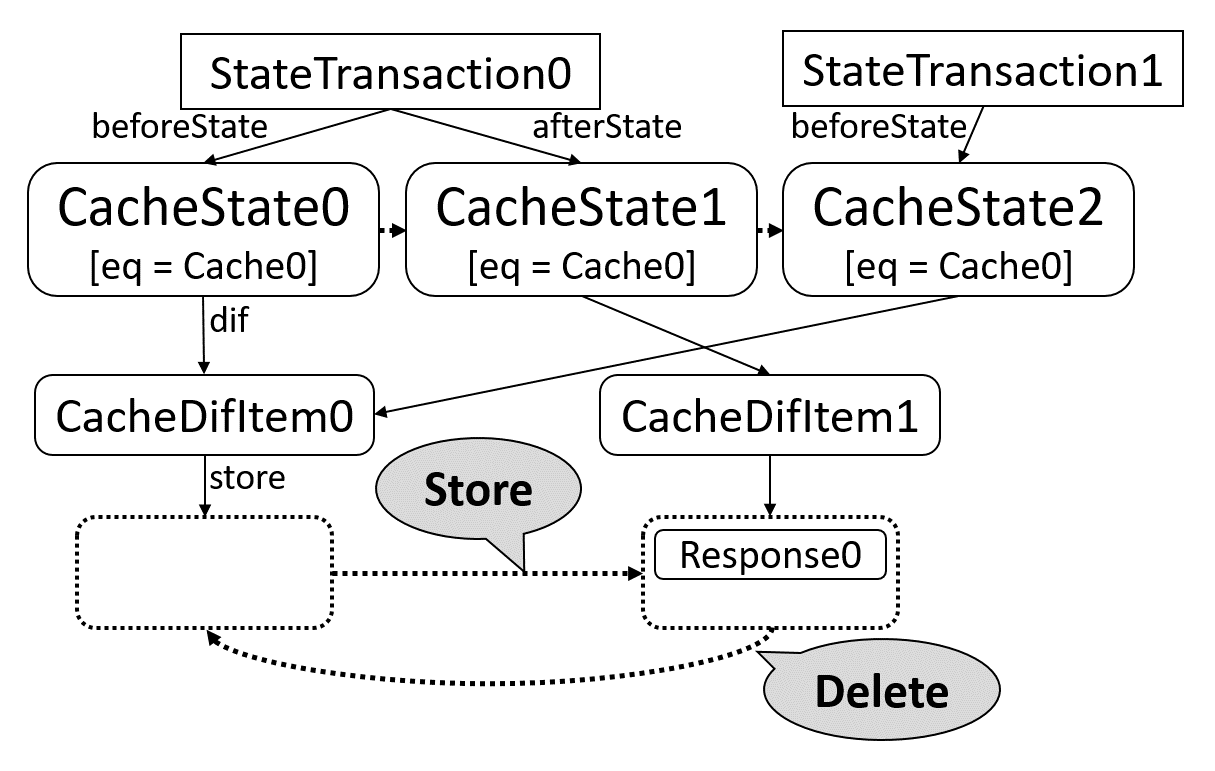
\includegraphics[width=\hsize]{./fig/ProposedModel-ResponseStoreDelete.eps}
\caption{キャッシュの格納と削除の表現}
\label{fig:ProposedModel-ResponseStoreDelete}
\end{figure}

また、以上の内容を提案モデルではCode\ref{code:StoreResponse}のように実装している。
すべてのCacheStateクラスのpostに対して、述語LastStateを用いて直前状態を取得し、それをpreとする。
ここでpostがリクエスト時の状態である場合、postの格納レスポンスの集合はpreの格納レスポンスの集合の補集合となる。
ここで、補集合とすることで前状態の格納レスポンスの一部がなくなることを容認し、格納レスポンスの削除を表現している。
また、postがレスポンス時の状態である場合、postの格納レスポンスの集合はpreの格納レスポンスの集合にpost時のレスポンスを加えた集合の補集合となる。
ここで、post時のレスポンスが集合に追加されることが、レスポンスの格納動作を表現している。

ただしこの記述のみでは各時点でのキャッシュの状態はその前状態に依存することになり、初期状態が無条件となる。
実際には、この場合の初期状態とはウェブ上における様々な通信が行われる前の状態を示すため、初期状態でキャッシュにレスポンスが格納されていることはない。
したがって、初期状態の格納レスポンスの集合を空集合とする制限を、述語InitailStateを用いて記述している。

\begin{lstlisting}[caption=レスポンスの格納と削除の表現, label=code:StoreResponse]
fact flowCacheState{
	all cs:CacheState |
		InitialState[cs] implies
			no cs.dif.store

	all pre, post:CacheState, str:StateTransaction |
		LastState[pre, post, str] implies {
			post in str.beforeState implies post.dif.store in pre.dif.store
			post in str.afterState implies post.dif.store in (pre.dif.store + str.response)
		}
}
\end{lstlisting}

\subsubsection{レスポンスの再利用}
提案モデルにおいて、キャッシュによるレスポンスの再利用は以下の動作を示す。

\begin{itembox}[l]{レスポンスの再利用}
キャッシュは、そのキャッシュが存在する端末が送受信するリクエストに対して、キャッシュ内の格納レスポンスで応答できる場合、そのレスポンスを用いて応答することができる。
ここで、リクエストの送信者が自身のキャッシュで再利用を行う場合、リクエストは実際はネットワーク上に発信されない。
\end{itembox}

上記で定めたレスポンスの再利用は、提案モデル内では本来発生するレスポンスの代わりとなって発生する。
したがって、既存モデルにおいてレスポンスを表すHTTPResponseクラスと同列に、CacheReuseクラスを定義する(Code\ref{code:CacheReuseClass}参照)。
HTTPResponseクラスはHTTPプロトコル上のイベントを表すHTTPEventクラスを継承しているため、CacheReuseクラスもHTTPEventクラスを継承する。
そして、CacheReuseクラスにある一つのレスポンスを関連付けることで、どのレスポンスを再利用したかを表現する。
また、HTTPEventクラスにおいて、どの端末からどの端末に対するイベントであるかは定義されており、これを利用することで再利用したレスポンスの送信元と送信先を表現する。
しかし、HTTPEventクラスでは送信元と送信先の他に、そのイベントに含まれるヘッダとボディが定義されている。
実際のレスポンスの再利用では、送信されるのは再利用するレスポンスのヘッダとボディであり、それは上記の再利用対象のレスポンスとの関連付けで表現されているためこの二項目は不必要である。
したがって、CacheReuseクラスとヘッダとボディの関係性は無視することができるが、ヘッダやボディを表すインスタンスは非常に多いため、無制限とした場合には無駄な計算時間を要することとなる。
このような要因から、CacheReuseクラスのヘッダとボディは空集合とし、計算時間の短縮を図る。

\begin{lstlisting}[caption=CacheReuseクラス, label=code:CacheReuseClass]
sig HTTPResponse extends HTTPEvent {
	statusCode: one Status
}
sig CacheReuse extends HTTPEvent{
	target: one HTTPResponse
}{
	no headers
	no body
}
\end{lstlisting}

上記で定義したCacheReuseクラスを用いて再利用を表現するため、CacheReuseイベントが発生する条件を、実際のキャッシュの動作に基づいて以下のように作成する。
\begin{itemize}
\item 再利用レスポンスの送信先は、その再利用を発生させたリクエストの送信元である
\item 再利用レスポンスの送信元は、その再利用を発生させたリクエストの送信元か送信先のいずれかである
\item 再利用を行うキャッシュの再利用直前の状態において、再利用するレスポンスが格納レスポンスに含まれている
\item 再利用するレスポンスと、その再利用を発生させたリクエストが表すURIが一致している
\end{itemize}

上記の条件の二点目において、再利用レスポンスの送信元がリクエストの送信元となる場合を認めるのは、そのリクエストを送信した端末のキャッシュによるレスポンスの再利用を想定するためである。

\subsubsection{格納レスポンスの検証}
\label{sec:CacheVerification}
提案モデルにおいて、キャッシュによる格納レスポンスの検証を以下のように定義する。

\begin{itembox}[l]{格納レスポンスの検証}
格納レスポンスは、格納レスポンスが再利用可能であるかを判定するために、条件付きリクエストを送信しオリジンサーバに問い合わせを行う。
条件付きリクエストは、if-modified-sinceヘッダかif-none-matchヘッダのいずれかが含まれるリクエストのことを指す。
これらのヘッダで送信される値を用いることで、オリジンサーバは格納レスポンスが最新のものと同一であるかを判定でき、再利用の可否をレスポンスで送信する。
検証が正常に終了した場合、このレスポンスの状態コードは304か200となる。
状態コードが304である場合は、そのヘッダやボディの値に関係なくキャッシュは格納レスポンスを再利用できる。
状態コードが200である場合は、格納レスポンスは再利用不可であり、このレスポンスをキャッシュに格納して再利用する。
また、検証後はどちらの場合も再利用可能なレスポンスの一つを除いて、同一のURIに対するレスポンスはキャッシュ内には存在しない。
\end{itembox}

この動作の実装は以下の二つを表現することで実現できる。
\begin{itemize}
\item レスポンスの再利用が行われている場合に、その再利用レスポンスが検証済みであるかを判定する述語
\item 条件付きリクエストに対するサーバの動作
\end{itemize}

まず、検証済みかを判定する述語checkVerificationをCode\ref{code:checkVerification}に示す。
この述語checkVerificationはStateTransaction(strとする)を入力とする。
述語checkVerificationは、strが再利用によって応答されているトランザクションであり、かつ、strのリクエストと再利用の間に条件付きリクエストを含むトランザクションが成立している場合に真となるように作成し、その論理は以下のように表せる。

\begin{itembox}[l]{述語checkVerification}
入力であるStateTransactionクラスのインスタンスstrが再利用を行っており、かつ、以下を満たすStateTranactionのクラスのインスタンスstr'が存在する場合に、本述語は真となる。
\begin{itemize}
\item strとstr'は異なるトランザクションである
\item str'のレスポンスが存在する。つまり、通信が正常に完了している
\item str'のリクエストはstrの後に発生し、str'のレスポンスはstrの再利用より前に発生している
\item str'のリクエストは、strの再利用が行われるキャッシュが属する端末から、再利用するレスポンスの送信元に送信されている
\item strとstr'での要求URIが同一である
\item 検証対象の格納レスポンスにetagヘッダかlast-modifiedヘッダが含まれている
\item 検証対象の格納レスポンスにetagヘッダが含まれている場合、str'のリクエストにif-none-matchヘッダが含まれる
\item 検証対象の格納レスポンスにlast-modifiedヘッダが含まれている場合、str'のリクエストにif-modified-sinceヘッダが含まれる
\end{itemize}
\end{itembox}

また、条件付きリクエストに関するサーバの動作をAlloy上で表現する。
HTTPTransactionクラスのインスタンスtrが条件付きリクエストを含む通信である場合、そのリクエストを受信したサーバは以下を満たすように条件を付加する。
\begin{itemize}
\item 検証後に、その検証対象のレスポンスのURIを持つ格納レスポンスは一つとなる
\item trのレスポンスの状態コードは200か304である
\item trのレスポンスの状態コードが200である場合、trのレスポンスはキャッシュに格納される
\item trのレスポンスの状態コードが304である場合、trのレスポンスはキャッシュに格納されない
\end{itemize}

\subsection{中継者の実装}
提案モデルにおいて中継者はHTTP/HTTPSプロトコルで動作し、プロキシとゲートウェイを包括する。
したがって、HTTPに遵守する端末を表すHTTPConfirmistを継承する形で中継者のクラスを宣言する。
また、中継者のクラスを継承し、プロキシとゲートウェイのクラスを宣言する。
これらのクラスは以下のコードで実装される。

\begin{lstlisting}[caption=中継者のクラス, label=code:IntermediaryClass]
abstract sig HTTPIntermediary extends HTTPConformist{}
sig HTTPProxy extends HTTPIntermediary{}
sig HTTPGateway extends HTTPIntermediary{}
\end{lstlisting}

また、この中継者の動作をAlloyで記述する。
中継者の動作はリクエストの送信先がHTTPIntermediaryであり、かつ、レスポンスが存在するHTTPTransactionに対する条件として記述できる。
このようなHTTPTransactionのインスタンスtrに対して、以下を満たすHTTPTransactionのインスタンスtr'が少なくとも一つ存在する。
\begin{itemize}
\item trとtr'は異なるトランザクションである
\item tr'のリクエストはtrのリクエストの後に発生し、tr'のレスポンスはtrのレスポンスの前に発生する
\item tr'のリクエストの送信元は、trのリクエストの送信先である中継者である
\item trとtr'のリクエストのURIは同一である
\item trとtr'のレスポンスのbodyと状態コードは同一である
\end{itemize}
ただし、上記の動作は正当なユーザに管理された中継者の動作であり、攻撃者が管理する中継者のふるまいはこの限りではない。

\end{document}

%\documentclass[journal]{IEEEtran}
\usepackage[dvipdfmx]{graphicx}
\usepackage{ascmac}
\usepackage{docmute}
\usepackage{comment}
\usepackage{listings}
\usepackage{listings}
\lstset{
	%枠外での自動改行
 	breaklines = true,
 	%標準の書体
 	%basicstyle = {\small},
 	%枠 "t"は上に線を記載, "T"は上に二重線を記載
	%他オプション:leftline,topline,bottomline,lines,single,shadowbox
 	frame = TB,
 	%タブの大きさ
 	tabsize = 2,
 	%キャプションの場所("tb"ならば上下両方に記載)
 	%captionpos = t,
 	%行番号の位置
 	%numbers = left,
 	%自動改行後のインデント量(デフォルトでは20[pt])	
 	breakindent = 30pt,
	%左右の位置調整 	
 	xleftmargin=15pt,
 	xrightmargin=10pt,
	%プログラム言語(複数の言語に対応,C,C++も可)
 	%language = Python, 	
 	%背景色と透過度
 	%backgroundcolor={\color[gray]{.90}},
 	%コメントの書体
 	%commentstyle = {\itshape \color[cmyk]{1,0.4,1,0}},
 	%関数名等の色の設定
 	%classoffset = 0,
 	%キーワード(int, ifなど)の書体
 	%keywordstyle = {\bfseries \color[cmyk]{0,1,0,0}},
 	%表示する文字の書体
 	%stringstyle = {\ttfamily \color[rgb]{0,0,1}},
 	%frameまでの間隔(行番号とプログラムの間)
 	%framesep = 5pt,
 	%行番号の間隔
 	%stepnumber = 1,
	%行番号の書体
 	%numberstyle = \tiny,
}
\makeatletter
\def\lst@makecaption{%
  \def\@captype{table}%
  \@makecaption
}
\makeatother
\renewcommand{\lstlistingname}{Code}

% Some very useful LaTeX packages include:
% (uncomment the ones you want to load)


% *** MISC UTILITY PACKAGES ***
%
%\usepackage{ifpdf}
% Heiko Oberdiek's ifpdf.sty is very useful if you need conditional
% compilation based on whether the output is pdf or dvi.
% usage:
% \ifpdf
%   % pdf code
% \else
%   % dvi code
% \fi
% The latest version of ifpdf.sty can be obtained from:
% http://www.ctan.org/pkg/ifpdf
% Also, note that IEEEtran.cls V1.7 and later provides a builtin
% \ifCLASSINFOpdf conditional that works the same way.
% When switching from latex to pdflatex and vice-versa, the compiler may
% have to be run twice to clear warning/error messages.


% *** CITATION PACKAGES ***
%
\usepackage{cite}
% cite.sty was written by Donald Arseneau
% V1.6 and later of IEEEtran pre-defines the format of the cite.sty package
% \cite{} output to follow that of the IEEE. Loading the cite package will
% result in citation numbers being automatically sorted and properly
% "compressed/ranged". e.g., [1], [9], [2], [7], [5], [6] without using
% cite.sty will become [1], [2], [5]--[7], [9] using cite.sty. cite.sty's
% \cite will automatically add leading space, if needed. Use cite.sty's
% noadjust option (cite.sty V3.8 and later) if you want to turn this off
% such as if a citation ever needs to be enclosed in parenthesis.
% cite.sty is already installed on most LaTeX systems. Be sure and use
% version 5.0 (2009-03-20) and later if using hyperref.sty.
% The latest version can be obtained at:
% http://www.ctan.org/pkg/cite
% The documentation is contained in the cite.sty file itself.


% *** GRAPHICS RELATED PACKAGES ***
%
\ifCLASSINFOpdf
  % \usepackage[pdftex]{graphicx}
  % declare the path(s) where your graphic files are
  % \graphicspath{{../pdf/}{../jpeg/}}
  % and their extensions so you won't have to specify these with
  % every instance of \includegraphics
  % \DeclareGraphicsExtensions{.pdf,.jpeg,.png}
\else
  % or other class option (dvipsone, dvipdf, if not using dvips). graphicx
  % will default to the driver specified in the system graphics.cfg if no
  % driver is specified.
  % \usepackage[dvips]{graphicx}
  % declare the path(s) where your graphic files are
  % \graphicspath{{../eps/}}
  % and their extensions so you won't have to specify these with
  % every instance of \includegraphics
  % \DeclareGraphicsExtensions{.eps}
\fi
% graphicx was written by David Carlisle and Sebastian Rahtz. It is
% required if you want graphics, photos, etc. graphicx.sty is already
% installed on most LaTeX systems. The latest version and documentation
% can be obtained at: 
% http://www.ctan.org/pkg/graphicx
% Another good source of documentation is "Using Imported Graphics in
% LaTeX2e" by Keith Reckdahl which can be found at:
% http://www.ctan.org/pkg/epslatex
%
% latex, and pdflatex in dvi mode, support graphics in encapsulated
% postscript (.eps) format. pdflatex in pdf mode supports graphics
% in .pdf, .jpeg, .png and .mps (metapost) formats. Users should ensure
% that all non-photo figures use a vector format (.eps, .pdf, .mps) and
% not a bitmapped formats (.jpeg, .png). The IEEE frowns on bitmapped formats
% which can result in "jaggedy"/blurry rendering of lines and letters as
% well as large increases in file sizes.
%
% You can find documentation about the pdfTeX application at:
% http://www.tug.org/applications/pdftex


% *** MATH PACKAGES ***
%
%\usepackage{amsmath}
% A popular package from the American Mathematical Society that provides
% many useful and powerful commands for dealing with mathematics.
%
% Note that the amsmath package sets \interdisplaylinepenalty to 10000
% thus preventing page breaks from occurring within multiline equations. Use:
%\interdisplaylinepenalty=2500
% after loading amsmath to restore such page breaks as IEEEtran.cls normally
% does. amsmath.sty is already installed on most LaTeX systems. The latest
% version and documentation can be obtained at:
% http://www.ctan.org/pkg/amsmath


% *** SPECIALIZED LIST PACKAGES ***
%
%\usepackage{algorithmic}
% algorithmic.sty was written by Peter Williams and Rogerio Brito.
% This package provides an algorithmic environment fo describing algorithms.
% You can use the algorithmic environment in-text or within a figure
% environment to provide for a floating algorithm. Do NOT use the algorithm
% floating environment provided by algorithm.sty (by the same authors) or
% algorithm2e.sty (by Christophe Fiorio) as the IEEE does not use dedicated
% algorithm float types and packages that provide these will not provide
% correct IEEE style captions. The latest version and documentation of
% algorithmic.sty can be obtained at:
% http://www.ctan.org/pkg/algorithms
% Also of interest may be the (relatively newer and more customizable)
% algorithmicx.sty package by Szasz Janos:
% http://www.ctan.org/pkg/algorithmicx


% *** ALIGNMENT PACKAGES ***
%
%\usepackage{array}
% Frank Mittelbach's and David Carlisle's array.sty patches and improves
% the standard LaTeX2e array and tabular environments to provide better
% appearance and additional user controls. As the default LaTeX2e table
% generation code is lacking to the point of almost being broken with
% respect to the quality of the end results, all users are strongly
% advised to use an enhanced (at the very least that provided by array.sty)
% set of table tools. array.sty is already installed on most systems. The
% latest version and documentation can be obtained at:
% http://www.ctan.org/pkg/array


% IEEEtran contains the IEEEeqnarray family of commands that can be used to
% generate multiline equations as well as matrices, tables, etc., of high
% quality.


% *** SUBFIGURE PACKAGES ***
%\ifCLASSOPTIONcompsoc
%  \usepackage[caption=false,font=normalsize,labelfont=sf,textfont=sf]{subfig}
%\else
%  \usepackage[caption=false,font=footnotesize]{subfig}
%\fi
% subfig.sty, written by Steven Douglas Cochran, is the modern replacement
% for subfigure.sty, the latter of which is no longer maintained and is
% incompatible with some LaTeX packages including fixltx2e. However,
% subfig.sty requires and automatically loads Axel Sommerfeldt's caption.sty
% which will override IEEEtran.cls' handling of captions and this will result
% in non-IEEE style figure/table captions. To prevent this problem, be sure
% and invoke subfig.sty's "caption=false" package option (available since
% subfig.sty version 1.3, 2005/06/28) as this is will preserve IEEEtran.cls
% handling of captions.
% Note that the Computer Society format requires a larger sans serif font
% than the serif footnote size font used in traditional IEEE formatting
% and thus the need to invoke different subfig.sty package options depending
% on whether compsoc mode has been enabled.
%
% The latest version and documentation of subfig.sty can be obtained at:
% http://www.ctan.org/pkg/subfig


% *** FLOAT PACKAGES ***
%
%\usepackage{fixltx2e}
% fixltx2e, the successor to the earlier fix2col.sty, was written by
% Frank Mittelbach and David Carlisle. This package corrects a few problems
% in the LaTeX2e kernel, the most notable of which is that in current
% LaTeX2e releases, the ordering of single and double column floats is not
% guaranteed to be preserved. Thus, an unpatched LaTeX2e can allow a
% single column figure to be placed prior to an earlier double column
% figure.
% Be aware that LaTeX2e kernels dated 2015 and later have fixltx2e.sty's
% corrections already built into the system in which case a warning will
% be issued if an attempt is made to load fixltx2e.sty as it is no longer
% needed.
% The latest version and documentation can be found at:
% http://www.ctan.org/pkg/fixltx2e


%\usepackage{stfloats}
% stfloats.sty was written by Sigitas Tolusis. This package gives LaTeX2e
% the ability to do double column floats at the bottom of the page as well
% as the top. (e.g., "\begin{figure*}[!b]" is not normally possible in
% LaTeX2e). It also provides a command:
%\fnbelowfloat
% to enable the placement of footnotes below bottom floats (the standard
% LaTeX2e kernel puts them above bottom floats). This is an invasive package
% which rewrites many portions of the LaTeX2e float routines. It may not work
% with other packages that modify the LaTeX2e float routines. The latest
% version and documentation can be obtained at:
% http://www.ctan.org/pkg/stfloats
% Do not use the stfloats baselinefloat ability as the IEEE does not allow
% \baselineskip to stretch. Authors submitting work to the IEEE should note
% that the IEEE rarely uses double column equations and that authors should try
% to avoid such use. Do not be tempted to use the cuted.sty or midfloat.sty
% packages (also by Sigitas Tolusis) as the IEEE does not format its papers in
% such ways.
% Do not attempt to use stfloats with fixltx2e as they are incompatible.
% Instead, use Morten Hogholm'a dblfloatfix which combines the features
% of both fixltx2e and stfloats:
%
% \usepackage{dblfloatfix}
% The latest version can be found at:
% http://www.ctan.org/pkg/dblfloatfix


%\ifCLASSOPTIONcaptionsoff
%  \usepackage[nomarkers]{endfloat}
% \let\MYoriglatexcaption\caption
% \renewcommand{\caption}[2][\relax]{\MYoriglatexcaption[#2]{#2}}
%\fi
% endfloat.sty was written by James Darrell McCauley, Jeff Goldberg and 
% Axel Sommerfeldt. This package may be useful when used in conjunction with 
% IEEEtran.cls'  captionsoff option. Some IEEE journals/societies require that
% submissions have lists of figures/tables at the end of the paper and that
% figures/tables without any captions are placed on a page by themselves at
% the end of the document. If needed, the draftcls IEEEtran class option or
% \CLASSINPUTbaselinestretch interface can be used to increase the line
% spacing as well. Be sure and use the nomarkers option of endfloat to
% prevent endfloat from "marking" where the figures would have been placed
% in the text. The two hack lines of code above are a slight modification of
% that suggested by in the endfloat docs (section 8.4.1) to ensure that
% the full captions always appear in the list of figures/tables - even if
% the user used the short optional argument of \caption[]{}.
% IEEE papers do not typically make use of \caption[]'s optional argument,
% so this should not be an issue. A similar trick can be used to disable
% captions of packages such as subfig.sty that lack options to turn off
% the subcaptions:
% For subfig.sty:
% \let\MYorigsubfloat\subfloat
% \renewcommand{\subfloat}[2][\relax]{\MYorigsubfloat[]{#2}}
% However, the above trick will not work if both optional arguments of
% the \subfloat command are used. Furthermore, there needs to be a
% description of each subfigure *somewhere* and endfloat does not add
% subfigure captions to its list of figures. Thus, the best approach is to
% avoid the use of subfigure captions (many IEEE journals avoid them anyway)
% and instead reference/explain all the subfigures within the main caption.
% The latest version of endfloat.sty and its documentation can obtained at:
% http://www.ctan.org/pkg/endfloat
%
% The IEEEtran \ifCLASSOPTIONcaptionsoff conditional can also be used
% later in the document, say, to conditionally put the References on a 
% page by themselves.


% *** PDF, URL AND HYPERLINK PACKAGES ***
%
%\usepackage{url}
% url.sty was written by Donald Arseneau. It provides better support for
% handling and breaking URLs. url.sty is already installed on most LaTeX
% systems. The latest version and documentation can be obtained at:
% http://www.ctan.org/pkg/url
% Basically, \url{my_url_here}.

\begin{document}

\section{事例研究}
本章では、複数の具体的な事例を取り上げ、提案モデルの表現能力の向上を確認する。

\subsection{キャッシュの基本動作}
本節では、提案モデルでキャッシュの動作の表現の可能性を確認する。
提案モデルにおいて、キャッシュは格納、再利用、検証の三つの動作を行うため、それぞれについてAlloy Analyzerの実行結果を確認する。

\subsubsection{レスポンスの格納}
レスポンスの格納動作を確認するため、実行結果からレスポンスの格納を含む結果を抽出する。
ここでは簡単のため、最も単純な二者間における通信で生じるレスポンスの格納を対象とし、Code\ref{code:test_store}を用いて出力を得る。
Code\ref{code:test_store}はクライアントとサーバの二者間における一組のリクエストとレスポンスの通信において、格納レスポンス集合に要素が存在するキャッシュの状態が存在する結果を出力するものである。

\begin{lstlisting}[caption=レスポンスの格納, label=code:test_store]
run test_store{
	#HTTPClient = 1
	#HTTPServer = 1
	#HTTPRequest = 1
	#HTTPResponse = 1
	some CacheState.dif.store
} for 2
\end{lstlisting}

得られる出力結果を整理し、図\ref{fig:TestStore}に示す。
図\ref{fig:TestStore}には、PrivateCache0を持つBrowser0とServer0間の、Request0とResponse0のトランザクションにおけるキャッシュの状態変化が示されている。
最初のRequest0時にはキャッシュの状態はCacheState0で示されており、CacheState0の変化要素を表すCacheDifItem0のstoreは空集合である。
しかし、Response0時には状態はCacheState1に変化しており、対応するCacheDifItem1がResponse0にstoreを指している。
以上より、図\ref{fig:TestStore}はあるトランザクションにおいて、レスポンスがブラウザキャッシュに格納されている状態を表しており、レスポンスの格納が表現可能であることが確認できる。

%\begin{figure}[htb]
%\centering
%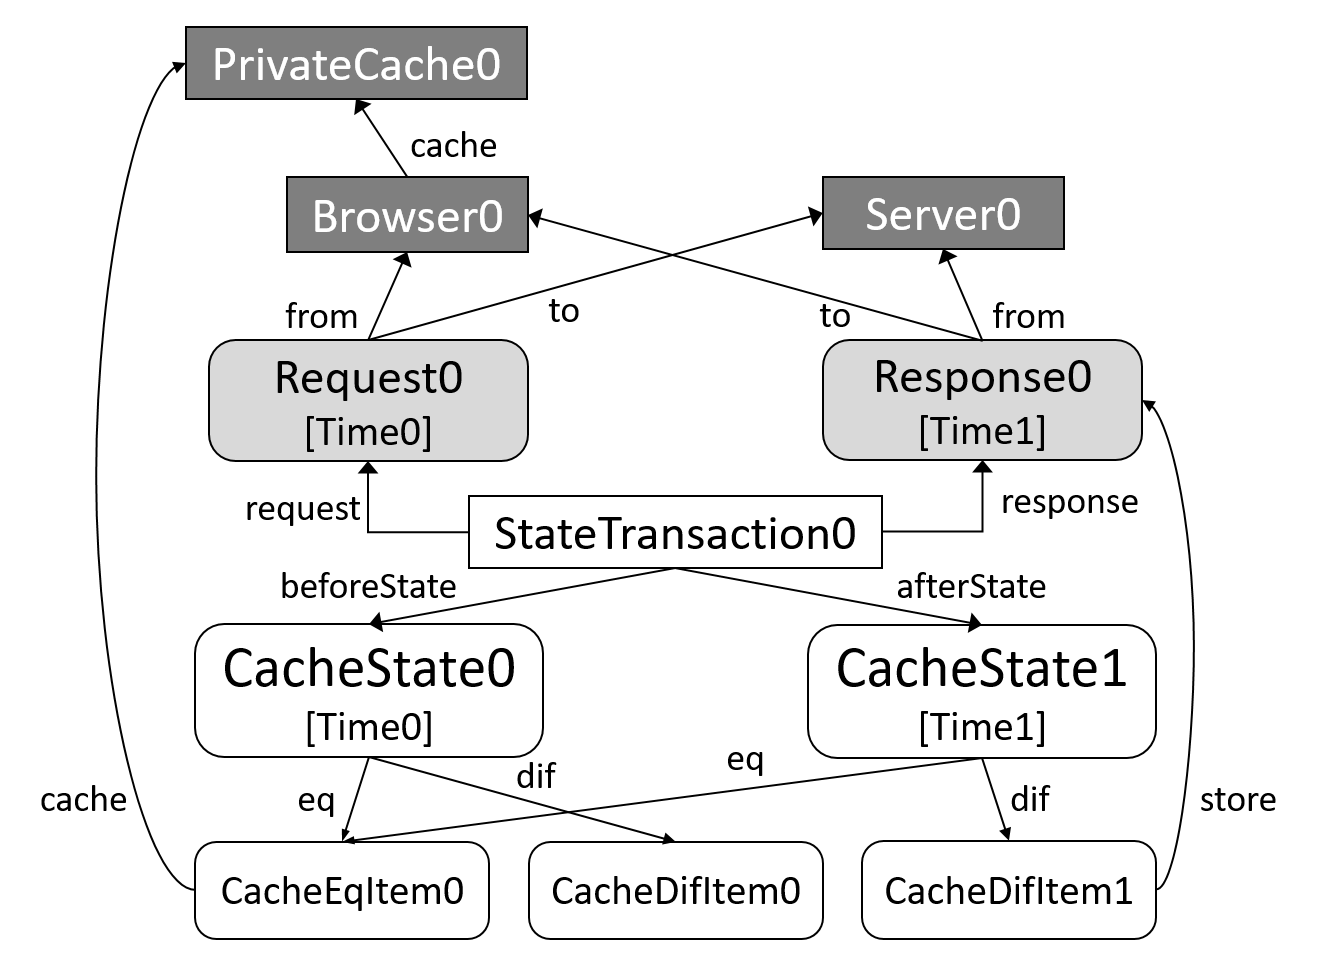
\includegraphics[width=450pt]{./fig/TestStore.eps}
%\caption{レスポンスを格納する状態の一例}
%\label{fig:TestStore}
%\end{figure}

\subsubsection{格納レスポンスの再利用}
レスポンスの再利用動作を確認するため、実行結果からレスポンスの再利用を含む結果を抽出する。
ここでは簡単のため、最も単純な二者間における通信で生じるレスポンスの再利用を対象とし、Code\ref{code:test_reuse}を用いて出力を得る。
Code\ref{code:test_reuse}はクライアントとサーバの二者間における二組の通信において、一度レスポンスの再利用が発生している結果を出力するものである。

\begin{lstlisting}[caption=格納レスポンスの再利用, label=code:test_reuse]
run test_reuse{
	#HTTPClient = 1
	#HTTPServer = 1
	#Cache = 1

	#HTTPRequest = 2
	#HTTPResponse = 1
	#CacheReuse = 1
} for 4
\end{lstlisting}

得られる出力結果をスペースの都合上、一部簡略化し図\ref{fig:TestReuse}に示す。
図\ref{fig:TestReuse}はあるキャッシュを持つブラウザとサーバ間で、同様のURIに対してリクエストが二回送信された状態を表している。
ここで、StateTransaction0では図\ref{fig:TestStore}と同様、ブラウザキャッシュにResponse0を格納している。
StateTransaction1では、この格納レスポンスを再利用するイベントCacheReuse0が発生している。
以上より、図\ref{fig:TestReuse}に示す出力結果から、再利用を伴う動作が表現可能であることが確認できる。

%\begin{figure}[htb]
%\centering
%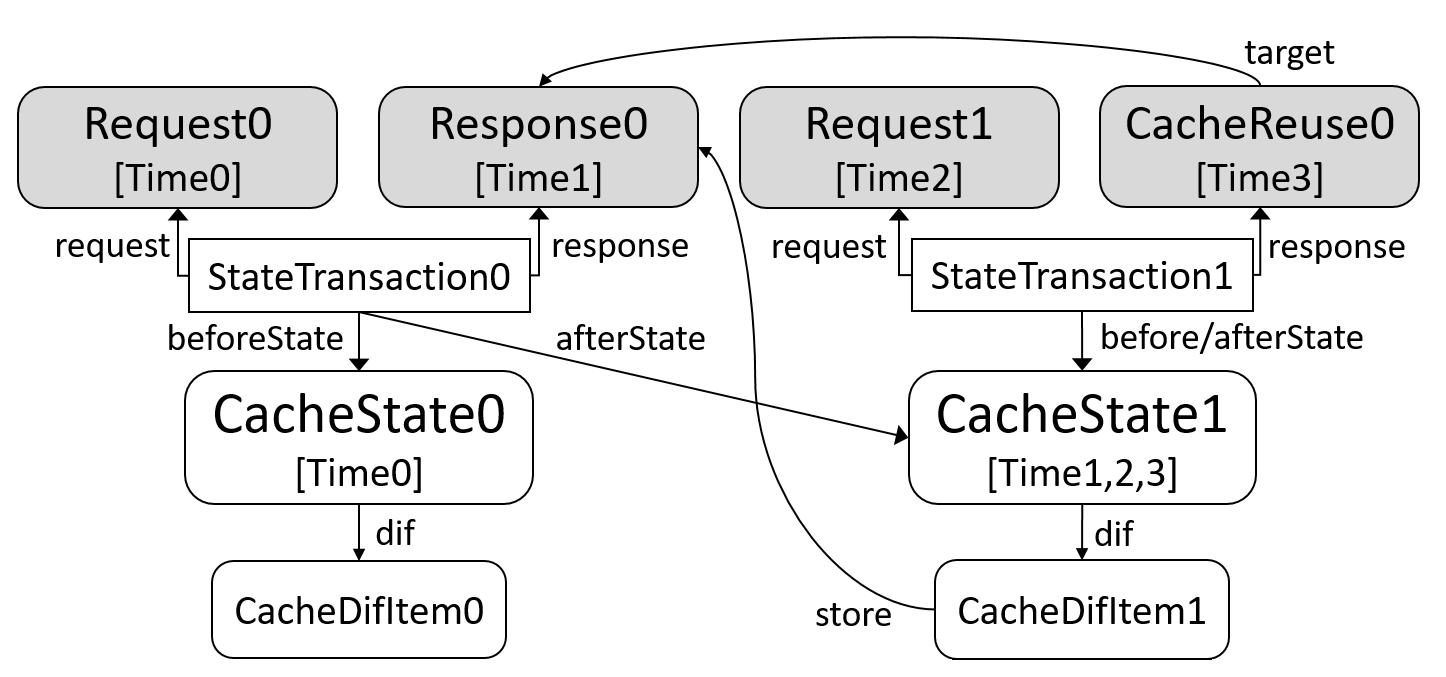
\includegraphics[width=450pt]{./fig/TestReuse.eps}
%\caption{格納レスポンスを再利用する状態の一例}
%\label{fig:TestReuse}
%\end{figure}

\subsubsection{格納レスポンスの検証}
レスポンスの検証動作を確認するため、実行結果からレスポンスの検証を含む結果を抽出する。
ここでは簡単のため、最も単純な二者間における通信で生じるレスポンスの検証を対象とし、Code\ref{code:test_verification}を用いて出力を得る。
Code\ref{code:test_verification}はクライアントとサーバの二者間における三組の通信のうち、検証が行われた通信が存在する結果を出力する。
ここでの検証の有無の判定は、\ref{sec:CacheVerification}節で述べた述語(Code\ref{code:checkVerification}参照)を利用している。

\begin{lstlisting}[caption=格納レスポンスの検証, label=code:test_verification]
run test_verification{
	#HTTPClient = 1
	#HTTPServer = 1
	#HTTPIntermediary = 0
	#Cache = 1
	#PrivateCache = 1

	some str:StateTransaction | checkVerification[str]
} for 6
\end{lstlisting}

得られる出力結果をスペースの都合上、一部簡略化し図\ref{fig:TestVerification}に示す。
図\ref{fig:TestVerification}はあるキャッシュを持つブラウザとサーバ間での三つの通信(StateTransaction0,1,2)が存在している状態を表しており、このうちStateTransaction2が検証を行っている通信である。
まず、StateTransaction0では図\ref{fig:TestStore}と同様、ブラウザキャッシュにResponse0を格納している。
次に、Request2に対してブラウザキャッシュ内に格納されているResponse0を再利用するため、StateTransaction2で検証動作を行っている。
ここで、格納レスポンスのResponse0にはEtagHeaderが含まれているため、検証に用いる条件付きリクエストであるRequest1にはIfNoneMatchHeaderが含まれている。
また、検証結果となるResponse1は再利用可能であることを示す304の状態コードとなっているため、Response0はそのまま再利用可能であることが示されている。
以上の流れからStateTransaction1ではResponse0をそのまま再利用しており、検証動作が正常に完了したことを示している。
よって、検証動作を表現可能であることが確認できる。

%\begin{figure}[htb]
%\centering
%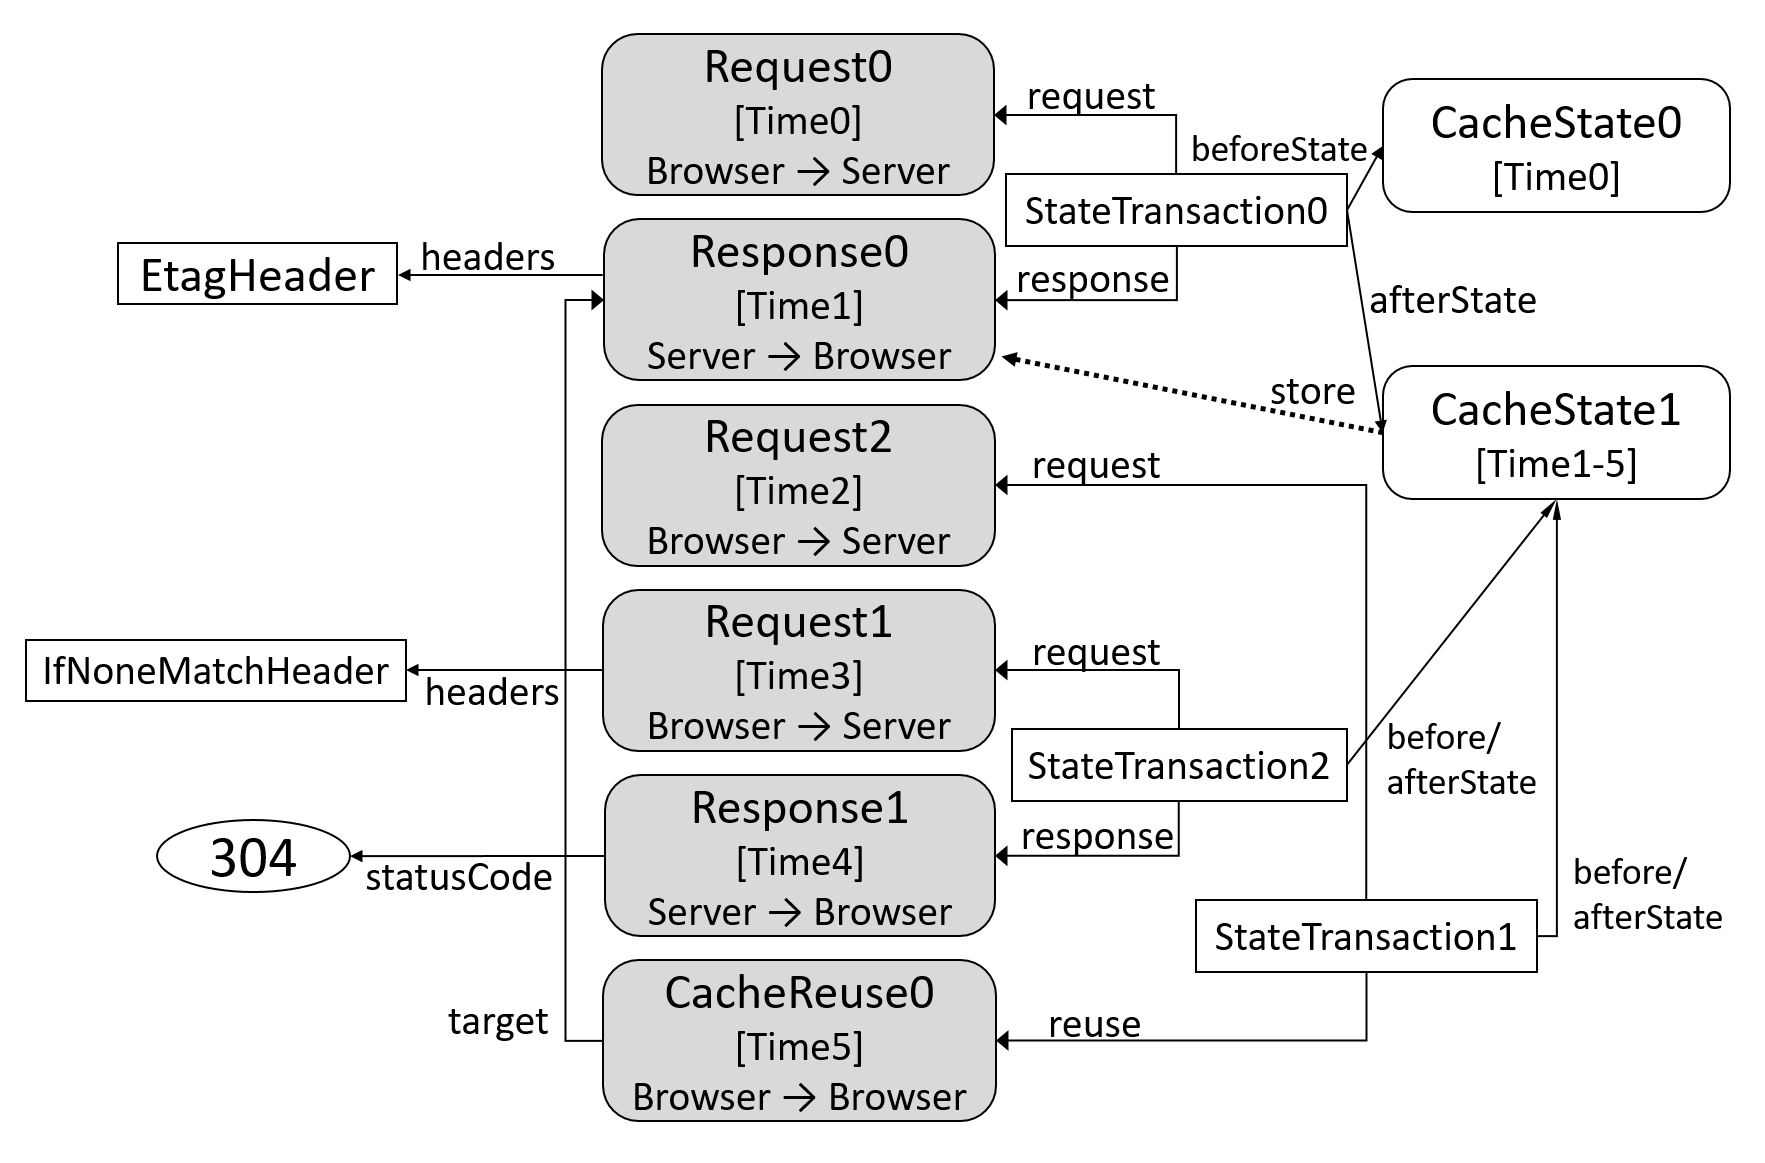
\includegraphics[width=450pt]{./fig/TestVerification.eps}
%\caption{格納レスポンスの検証が含まれる状態の一例}
%\label{fig:TestVerification}
%\end{figure}

\subsection{中継者の基本動作}
中継者の動作を確認するため、実行結果から中継者の動作を伴う動作を含む結果を抽出する。
ここでは簡単のため、最も単純なクライアント、中継者、サーバが各一つずつ存在する経路において、中継者を経由する通信を対象としCode\ref{code:test_intermediary}を用いて出力を得る。

\begin{lstlisting}[caption=中継者の動作, label=code:test_intermediary]
run test_intermediary{
	#HTTPRequest = 2
	#HTTPResponse = 2

	#HTTPClient = 1
	#HTTPServer = 1
	#HTTPIntermediary = 1

	all i:HTTPIntermediary | i in Alice.servers

	one req:HTTPRequest | req.to in HTTPIntermediary
	one req:HTTPRequest | req.to in HTTPServer
} for 4
\end{lstlisting}

得られる出力結果をスペースの都合上、一部簡略化し図\ref{fig:TestIntermediary}に示す。
図\ref{fig:TestIntermediary}で、HTTPTransaction0はブラウザと中継者間の通信、HTTPTransaction1は中継者とサーバ間の通信を表す。
中継者は自身に届けられたリクエストやレスポンスを回送する役割を持ち、このHTTPTransaction1がHTTPTransaction0を改装していることを表している。
以上より、中継者の動作が表現可能であることが確認できる。

%\begin{figure}[htb]
%\centering
%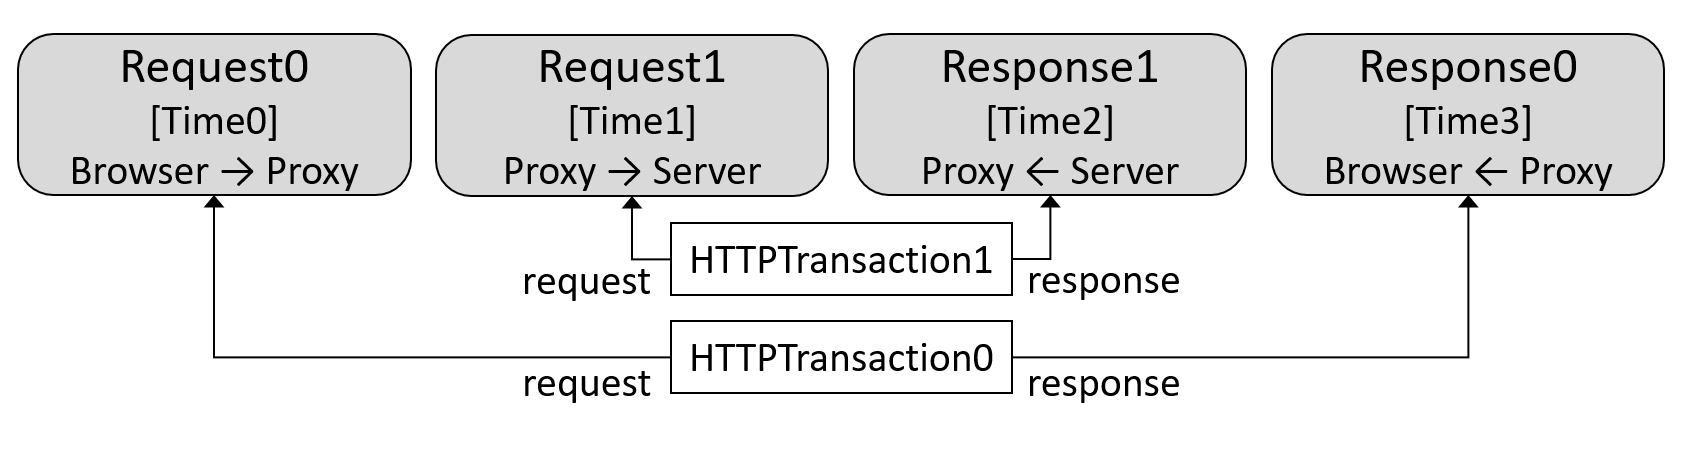
\includegraphics[width=450pt]{./fig/TestIntermediary.eps}
%\caption{中継者の動作を含む状態の一例}
%\label{fig:TestIntermediary}
%\end{figure}

\subsection{Same-origin Browser Cache Poisoning Attack}
\label{sec:same-origin-bcp}
本節では、提案モデルでSame-origin Browser Cache Poisoning Attack\cite{bcpattack}(以下、Same-origin BCP攻撃とする)が表現可能であるかを確認する。

Same-origin BCP攻撃は、攻撃者の持つ中継者が攻撃対象であるブラウザとサーバの経路上に入り込む「中間者攻撃」の一種である。
本攻撃の目的は対象のブラウザ、攻撃者の任意の動作を実行させることを目的とする。
また、本攻撃の特徴は、攻撃者による通信経路の割り込みが一度であるにも関わらず、そのレスポンスを再利用するたびにブラウザが悪影響を受けるという影響の持続性にある。

攻撃全体のフローを図\ref{fig:SameBCP_flow}に示す。
本攻撃による攻撃者のふるまいは、通信経路上において本来ブラウザが受け取るはずのレスポンスの内容に改ざん(図\ref{fig:SameBCP_flow}内の「4.改ざんレスポンス」)を行い、ブラウザが保有するキャッシュに改ざんレスポンスを格納させることである。
この際の攻撃者による改ざん内容は以下の二点である。
\begin{itemize}
\item レスポンスのヘッダをブラウザキャッシュによるレスポンスの格納や再利用を誘発するよう改ざんする。例えば、有効期限の延長や、検証動作なしの再利用の許可が挙げられる
\item レスポンスのボディに攻撃者に実行させたい任意の動作を記述する
\end{itemize}
また、ブラウザに悪影響が及ぶのは「5.改ざんレスポンスをキャッシュに格納」時と「6.同じファイルの利用時に改ざんレスポンスを再利用」時である。
また、6は改ざんレスポンスがキャッシュ内に格納されている間、何度も繰り返される可能性がある。

%\begin{figure}[htb]
%\centering
%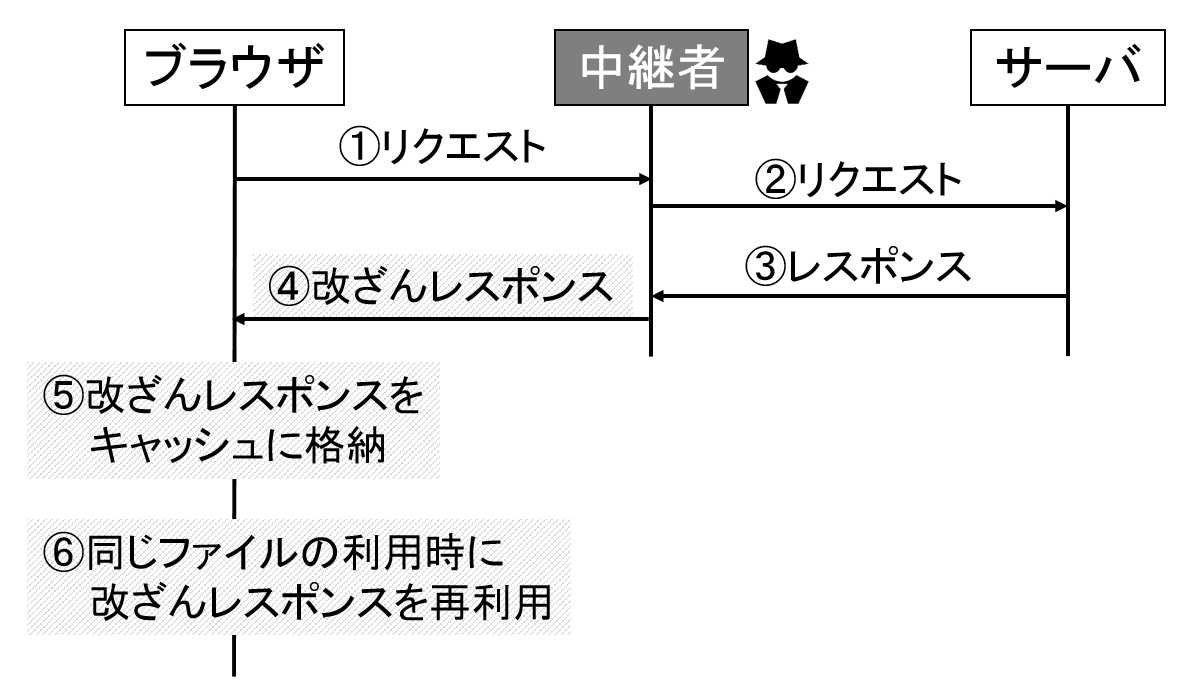
\includegraphics[width=400pt]{./fig/SameBCP_flow.eps}
%\caption{Same-origin Browser Cache Poisoning Attackの攻撃フロー}
%\label{fig:SameBCP_flow}
%\end{figure}

提案モデルによるSame-origin BCP攻撃の表現を確認するため、実行結果から図\ref{fig:SameBCP_flow}のフローを含む結果を抽出する。
抽出にはCode\ref{code:Same_origin_BCP}を用いる。
実行結果として、図\ref{fig:SameBCP_flow}に従ったフローと、攻撃者によるヘッダとボディの改ざんを含む状態が得られた。
このことから、提案モデルがSame-origin BCP攻撃を表現できることを確認した。

\begin{lstlisting}[caption=Same-origin BCP攻撃の表現, label=code:Same_origin_BCP]
run Same_origin_BCP{
	#HTTPClient = 1
	#HTTPServer = 1
	#HTTPIntermediary = 1
	#PrivateCache = 1
	#PublicCache = 0

	#HTTPRequest = 3
	#HTTPResponse = 2
	#CacheReuse = 1

	#Principal = 3
	#Alice = 2

	some tr,tr',tr'':HTTPTransaction | {
		tr'.request.current in tr.request.current.*next
		tr.response.current in tr'.response.current.*next
		tr''.request.current in tr.response.current.*next
		some tr''.re_res

		tr.request.from in HTTPClient
		tr.request.to in HTTPIntermediary

		tr'.request.from in HTTPIntermediary
		tr'.request.to in HTTPServer

		tr''.request.from in HTTPClient

		tr.response.body != tr'.response.body
	}

	some c:HTTPClient | c in Alice.httpClients
	some s:HTTPServer | s in Alice.servers
	no i:HTTPIntermediary | i in Alice.servers
} for 6
\end{lstlisting}

\subsection{Cross-site Request Forgery Attack}
本節では、提案モデルでCross-site Request Forgery Attack\cite{cookie-model}(以下、CSRF攻撃とする)が表現可能であるかを確認する。

CSRF攻撃は攻撃対象となるサーバと攻撃者が保有するサーバ、そして一般的なブラウザの三者間で実現される攻撃である。
本攻撃の目標は、攻撃対象であるサーバに対して、攻撃者が許されていない動作を実行させることである。

攻撃全体のフローを図\ref{fig:CSRF_flow}に示す。
本攻撃における攻撃者のふるまいは、自身が保有するサーバにアクセスしてきたブラウザが攻撃対象であるサーバへの「3.リクエスト」を送信を誘発するように「2.レスポンス」を返すことである。
また、この攻撃者からのレスポンスの内容によって、ブラウザから送信されるリクエストの内容も操作される。

%\begin{figure}[htb]
%\centering
%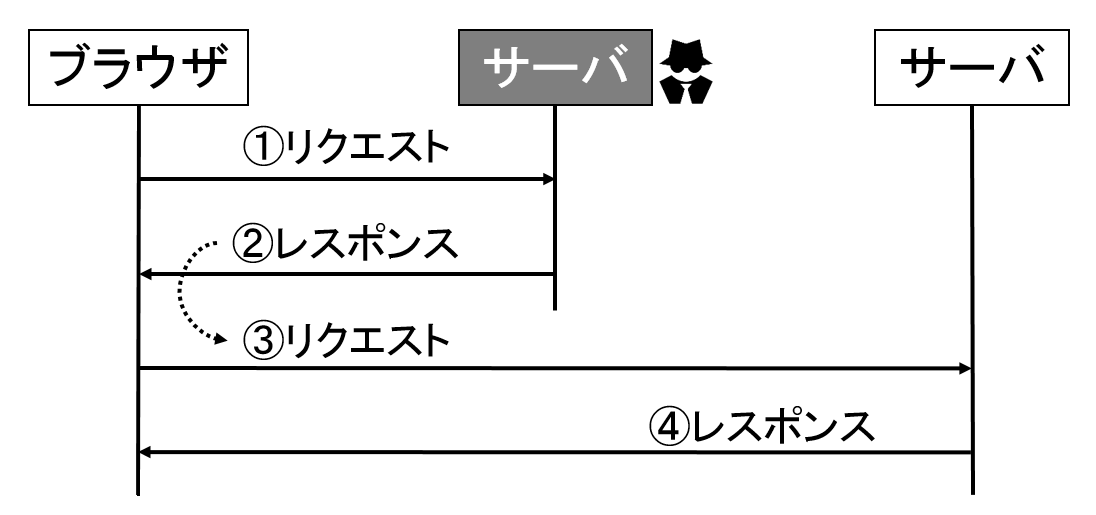
\includegraphics[width=400pt]{./fig/CSRF_flow.eps}
%\caption{Cross-site Request Forgery Attackの攻撃フロー}
%\label{fig:CSRF_flow}
%\end{figure}

提案モデルによるCSRF攻撃の表現を確認するため、実行結果から図\ref{fig:CSRF_flow}のフローを含む結果を抽出する。
抽出にはCode\ref{code:CSRF}を用い、その実行結果として図\ref{fig:CSRF_flow}に示す攻撃フローを含む結果が出力された。
スペースの都合上、これを一部簡略化し図\ref{fig:CSRF_alloy}に示す。
図\ref{fig:CSRF_alloy}において、Server0が攻撃者のサーバ、Server1が攻撃対象のサーバを表している。
また、HTTPTransaction0はBrowserがServer0にアクセスした通信を、HTTPTransaction1はそれに誘発されたBrowserとServer1の通信を表している。
HTTPTransaction1はHTTPTransaction0にcauseの関係を持ち、これがHTTPTransaction0に誘発されていることを示している。
以上のことから、CSRF攻撃を含む出力結果が得られているため、提案モデルがCSRF攻撃を表現できることを確認した。

\begin{lstlisting}[caption=CSRF攻撃の表現, label=code:CSRF]
run CSRF{
	#HTTPRequest = 2
	#HTTPResponse = 2

	#HTTPClient = 1
	#HTTPServer = 2
	#HTTPIntermediary = 0

	#Principal = 3
	#Alice = 2

	all p:Principal |
		one c:HTTPConformist |
			c in p.(servers + httpClients)
	all b:Browser | b in Alice.httpClients

	one tr1,tr2:HTTPTransaction|{
		tr2.request.current in tr1.response.current.*next

		tr1.request.to !in Alice.servers
		tr2.request.to in Alice.servers

		tr2.cause = tr1

		tr1.request.uri != tr2.request.uri
	}
} for 4
\end{lstlisting}

%\begin{figure}[htb]
%\centering
%\includegraphics[width=450pt]{./fig/CSRF_alloy.eps}
%\caption{CSRF攻撃のフローを含む状態の一例}
%\label{fig:CSRF_alloy}
%\end{figure}

\subsection{Cross-origin Browser Cache Poisoning Attack}
本節では、提案モデルでCross-origin Browser Cache Poisoning Attack\cite{bcpattack}(以下、Cross-origin BCP攻撃とする)が表現可能であるかを確認する。

Cross-origin BCP攻撃は、\ref{sec:same-origin-bcp}節で述べたSame-origin BCP攻撃と同様に「中間者攻撃」の一種である。
本攻撃法はSame-origin BCP攻撃に比べ、改ざんレスポンスの再利用の頻度を高めることができる。
これは、Cross-origin BCP攻撃では任意のファイルのレスポンスに改ざんを行うことができることに起因する。
これにより、一つのサイトだけでなく多くのサイトに共通して利用されるようなファイル(cssやjsファイルなど)を改ざんの対象とすることができる。
これに対して、\ref{sec:same-origin-bcp}節で記述のSame-origin BCP攻撃は、攻撃者がファイルを指定することはできず、通信に介入した際に偶然行われていた通信のみを改ざん可能な対象とする。

Cross-origin BCP攻撃は図\ref{fig:CrossBCP_flow}に示す攻撃フローで実現される。
ここで、図\ref{fig:CrossBCP_flow}内での「5.リクエスト」以降は、Same-origin BCP攻撃と同一のフローである。
また、それ以前のフローについては、CSRFのフローと役割が類似している。
まず最初に、攻撃者は「1.リクエスト」の通信に介入し、レスポンスの改ざんを行う。
ここにおける改ざんは、実際に改ざんを試みるファイルに対しての「5.リクエスト」の誘発を目的とする。
例えば、「A.css」という多くのページで共通して使用されるファイルが存在する場合、「3.レスポンス」の内容にA.cssを利用するよう追記することで、A.cssに対する「5.リクエスト」を誘発することができる。
したがって、図\ref{fig:CrossBCP_flow}のフローによって、攻撃者が指定する任意のファイルの改ざんを行い、そのレスポンスをブラウザキャッシュに格納させることができる。
また、このフローの成功後はサーバ1,2に無関係な通信であったとしても、改ざんレスポンスに記述されているファイルを利用する際には再利用が発生し、ブラウザは悪影響を受ける。

%\begin{figure}[htb]
%\centering
%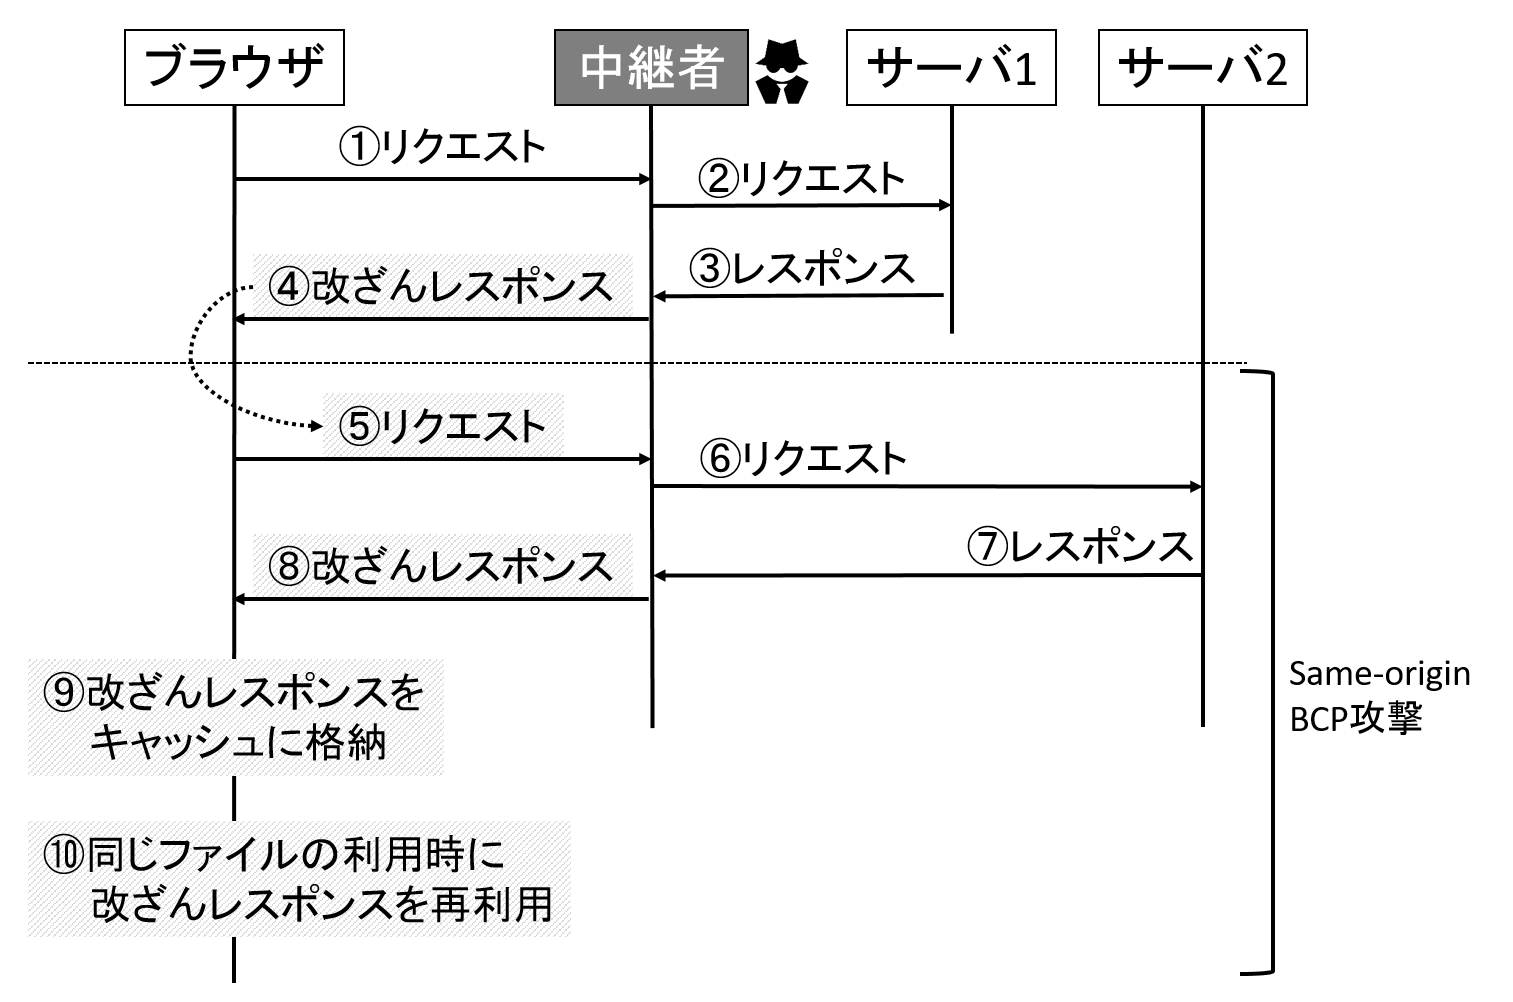
\includegraphics[width=450pt]{./fig/CrossBCP_flow.eps}
%\caption{Cross-origin Browser Cache Poisoning Attackの攻撃フロー}
%\label{fig:CrossBCP_flow}
%\end{figure}

提案モデルによるCross-origin BCP攻撃の表現を確認するため、実行結果から図\ref{fig:CrossBCP_flow}を含む結果を抽出する。
結果として、図\ref{fig:CrossBCP_flow}に存在する五つの通信を表現された状態を出力した。
このことから、提案モデルがCross-origin BCP攻撃を表現できることを確認した。
また、スペースの都合上、実行コードは巻末付録Code\ref{code:Cross_origin_BCP}に記載する。

\subsection{Web Cache Deception Attack}
本節では、提案モデルでWeb Cache Deception Attack\cite{WCD}(以下、WCD攻撃とする)が表現可能であるかを確認する。

WCD攻撃は攻撃対象となるサーバと中継者、二つのブラウザ間で成り立つ攻撃である。
攻撃者はこれらのうち一つのブラウザを所有し、本来、攻撃者がサーバから得ることのできないファイルを取得することが目的である。

WCD攻撃は図\ref{fig:WCD_flow}に示す攻撃フローで実現される。
まず、攻撃者にアクセス権の無いファイルに対して、正当なユーザに中継者を経由してアクセスさせる。
この際に、その「3.レスポンス」が中継者のキャッシュに格納された場合、攻撃者はその中継者を含む経路でそのファイルに対する「5.リクエスト」を送信することで、中継者のキャッシュによる「6.格納レスポンスの再利用」が発生しそのファイルを取得できる。

%\begin{figure}[htb]
%\centering
%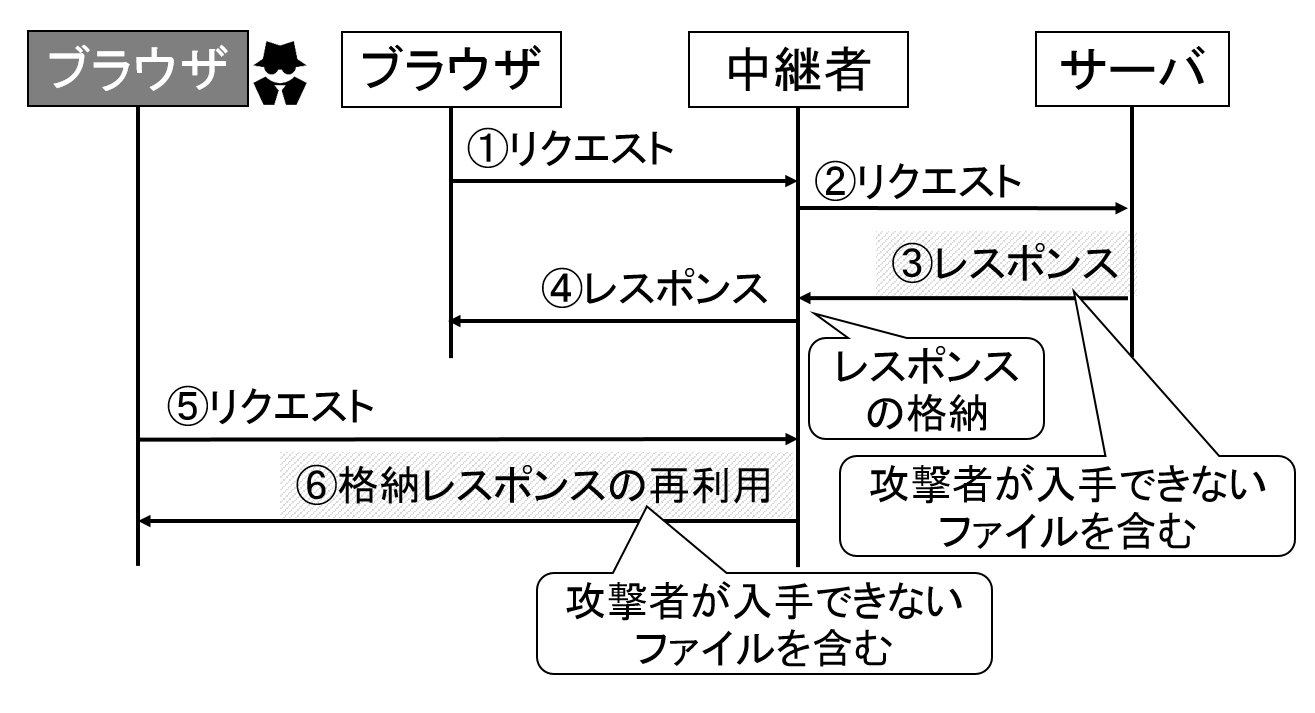
\includegraphics[width=450pt]{./fig/WCD_flow.eps}
%\caption{Web Cache Deception Attackの攻撃フロー}
%\label{fig:WCD_flow}
%\end{figure}

提案モデルによるWCD攻撃の表現を確認するため、実行結果から図\ref{fig:WCD_flow}のフローを含む結果を抽出する。
抽出にはCode\ref{code:WCD}を用い、その実行結果として図\ref{fig:WCD_flow}に示す攻撃フローを含む結果が出力された。
スペースの都合上、これを一部簡略化し図\ref{fig:WCD_alloy}に示す。
図\ref{fig:WCD_alloy}において、図\ref{fig:WCD_flow}の「1.リクエスト」と「2.リクエスト」の通信はStateTransaction0,1でそれぞれ表されている。
ここで、Response1のボディにはTokenが付与されており、これが攻撃者がアクセス権を持たないファイルを示している。
このResponse1は、その発生時刻Time2で中継者のキャッシュに保存され、攻撃者による通信StateTransaction2において再利用されている。
従って、この出力結果は攻撃者が本来権限を持たないファイルを中継者のキャッシュによる再利用を用いて取得していることを表している。
以上のことから、WCD攻撃を含む出力結果が得られているため、提案モデルがWCD攻撃を表現できることを確認した。

\begin{lstlisting}[caption=WCD攻撃の表現, label=code:WCD]
run Web_Cache_Deception{
	#HTTPRequest = 3
	#HTTPResponse = 2
	#CacheReuse = 1

	#HTTPClient = 2
	#HTTPServer = 1
	#HTTPProxy = 1
	#Cache = 1

	#Principal = 4
	#Alice = 3

	all c:Cache | c in HTTPProxy.cache

	all p:Principal |
		one c:HTTPConformist |
			c in p.(servers + httpClients)
	all i:HTTPProxy | i in Alice.servers
	all s:HTTPServer | s in Alice.servers

	one tr1,tr2,tr3:HTTPTransaction |{
		tr1.request.from in Alice.httpClients
		tr1.request.to in HTTPProxy

		tr2.request.from in HTTPProxy
		tr2.request.to in HTTPServer

		(tr3.request.from !in Alice.httpClients and tr3.request.from in HTTPClient)
		tr3.request.to in HTTPProxy

		one tr3.re_res
	}
} for 6
\end{lstlisting}

%\begin{figure}[htb]
%\centering
%\includegraphics[width=450pt]{./fig/WCD_alloy.eps}
%\caption{WCD攻撃のフローを含む状態の一例}
%\label{fig:WCD_alloy}
%\end{figure}

\end{document}

%\documentclass[journal]{IEEEtran}
\usepackage[dvipdfmx]{graphicx}
\usepackage{ascmac}
\usepackage{docmute}
\usepackage{comment}
\usepackage{listings}
\usepackage{listings}
\lstset{
	%枠外での自動改行
 	breaklines = true,
 	%標準の書体
 	%basicstyle = {\small},
 	%枠 "t"は上に線を記載, "T"は上に二重線を記載
	%他オプション:leftline,topline,bottomline,lines,single,shadowbox
 	frame = TB,
 	%タブの大きさ
 	tabsize = 2,
 	%キャプションの場所("tb"ならば上下両方に記載)
 	%captionpos = t,
 	%行番号の位置
 	%numbers = left,
 	%自動改行後のインデント量(デフォルトでは20[pt])	
 	breakindent = 30pt,
	%左右の位置調整 	
 	xleftmargin=15pt,
 	xrightmargin=10pt,
	%プログラム言語(複数の言語に対応,C,C++も可)
 	%language = Python, 	
 	%背景色と透過度
 	%backgroundcolor={\color[gray]{.90}},
 	%コメントの書体
 	%commentstyle = {\itshape \color[cmyk]{1,0.4,1,0}},
 	%関数名等の色の設定
 	%classoffset = 0,
 	%キーワード(int, ifなど)の書体
 	%keywordstyle = {\bfseries \color[cmyk]{0,1,0,0}},
 	%表示する文字の書体
 	%stringstyle = {\ttfamily \color[rgb]{0,0,1}},
 	%frameまでの間隔(行番号とプログラムの間)
 	%framesep = 5pt,
 	%行番号の間隔
 	%stepnumber = 1,
	%行番号の書体
 	%numberstyle = \tiny,
}
\makeatletter
\def\lst@makecaption{%
  \def\@captype{table}%
  \@makecaption
}
\makeatother
\renewcommand{\lstlistingname}{Code}

% Some very useful LaTeX packages include:
% (uncomment the ones you want to load)


% *** MISC UTILITY PACKAGES ***
%
%\usepackage{ifpdf}
% Heiko Oberdiek's ifpdf.sty is very useful if you need conditional
% compilation based on whether the output is pdf or dvi.
% usage:
% \ifpdf
%   % pdf code
% \else
%   % dvi code
% \fi
% The latest version of ifpdf.sty can be obtained from:
% http://www.ctan.org/pkg/ifpdf
% Also, note that IEEEtran.cls V1.7 and later provides a builtin
% \ifCLASSINFOpdf conditional that works the same way.
% When switching from latex to pdflatex and vice-versa, the compiler may
% have to be run twice to clear warning/error messages.


% *** CITATION PACKAGES ***
%
\usepackage{cite}
% cite.sty was written by Donald Arseneau
% V1.6 and later of IEEEtran pre-defines the format of the cite.sty package
% \cite{} output to follow that of the IEEE. Loading the cite package will
% result in citation numbers being automatically sorted and properly
% "compressed/ranged". e.g., [1], [9], [2], [7], [5], [6] without using
% cite.sty will become [1], [2], [5]--[7], [9] using cite.sty. cite.sty's
% \cite will automatically add leading space, if needed. Use cite.sty's
% noadjust option (cite.sty V3.8 and later) if you want to turn this off
% such as if a citation ever needs to be enclosed in parenthesis.
% cite.sty is already installed on most LaTeX systems. Be sure and use
% version 5.0 (2009-03-20) and later if using hyperref.sty.
% The latest version can be obtained at:
% http://www.ctan.org/pkg/cite
% The documentation is contained in the cite.sty file itself.


% *** GRAPHICS RELATED PACKAGES ***
%
\ifCLASSINFOpdf
  % \usepackage[pdftex]{graphicx}
  % declare the path(s) where your graphic files are
  % \graphicspath{{../pdf/}{../jpeg/}}
  % and their extensions so you won't have to specify these with
  % every instance of \includegraphics
  % \DeclareGraphicsExtensions{.pdf,.jpeg,.png}
\else
  % or other class option (dvipsone, dvipdf, if not using dvips). graphicx
  % will default to the driver specified in the system graphics.cfg if no
  % driver is specified.
  % \usepackage[dvips]{graphicx}
  % declare the path(s) where your graphic files are
  % \graphicspath{{../eps/}}
  % and their extensions so you won't have to specify these with
  % every instance of \includegraphics
  % \DeclareGraphicsExtensions{.eps}
\fi
% graphicx was written by David Carlisle and Sebastian Rahtz. It is
% required if you want graphics, photos, etc. graphicx.sty is already
% installed on most LaTeX systems. The latest version and documentation
% can be obtained at: 
% http://www.ctan.org/pkg/graphicx
% Another good source of documentation is "Using Imported Graphics in
% LaTeX2e" by Keith Reckdahl which can be found at:
% http://www.ctan.org/pkg/epslatex
%
% latex, and pdflatex in dvi mode, support graphics in encapsulated
% postscript (.eps) format. pdflatex in pdf mode supports graphics
% in .pdf, .jpeg, .png and .mps (metapost) formats. Users should ensure
% that all non-photo figures use a vector format (.eps, .pdf, .mps) and
% not a bitmapped formats (.jpeg, .png). The IEEE frowns on bitmapped formats
% which can result in "jaggedy"/blurry rendering of lines and letters as
% well as large increases in file sizes.
%
% You can find documentation about the pdfTeX application at:
% http://www.tug.org/applications/pdftex


% *** MATH PACKAGES ***
%
%\usepackage{amsmath}
% A popular package from the American Mathematical Society that provides
% many useful and powerful commands for dealing with mathematics.
%
% Note that the amsmath package sets \interdisplaylinepenalty to 10000
% thus preventing page breaks from occurring within multiline equations. Use:
%\interdisplaylinepenalty=2500
% after loading amsmath to restore such page breaks as IEEEtran.cls normally
% does. amsmath.sty is already installed on most LaTeX systems. The latest
% version and documentation can be obtained at:
% http://www.ctan.org/pkg/amsmath


% *** SPECIALIZED LIST PACKAGES ***
%
%\usepackage{algorithmic}
% algorithmic.sty was written by Peter Williams and Rogerio Brito.
% This package provides an algorithmic environment fo describing algorithms.
% You can use the algorithmic environment in-text or within a figure
% environment to provide for a floating algorithm. Do NOT use the algorithm
% floating environment provided by algorithm.sty (by the same authors) or
% algorithm2e.sty (by Christophe Fiorio) as the IEEE does not use dedicated
% algorithm float types and packages that provide these will not provide
% correct IEEE style captions. The latest version and documentation of
% algorithmic.sty can be obtained at:
% http://www.ctan.org/pkg/algorithms
% Also of interest may be the (relatively newer and more customizable)
% algorithmicx.sty package by Szasz Janos:
% http://www.ctan.org/pkg/algorithmicx


% *** ALIGNMENT PACKAGES ***
%
%\usepackage{array}
% Frank Mittelbach's and David Carlisle's array.sty patches and improves
% the standard LaTeX2e array and tabular environments to provide better
% appearance and additional user controls. As the default LaTeX2e table
% generation code is lacking to the point of almost being broken with
% respect to the quality of the end results, all users are strongly
% advised to use an enhanced (at the very least that provided by array.sty)
% set of table tools. array.sty is already installed on most systems. The
% latest version and documentation can be obtained at:
% http://www.ctan.org/pkg/array


% IEEEtran contains the IEEEeqnarray family of commands that can be used to
% generate multiline equations as well as matrices, tables, etc., of high
% quality.


% *** SUBFIGURE PACKAGES ***
%\ifCLASSOPTIONcompsoc
%  \usepackage[caption=false,font=normalsize,labelfont=sf,textfont=sf]{subfig}
%\else
%  \usepackage[caption=false,font=footnotesize]{subfig}
%\fi
% subfig.sty, written by Steven Douglas Cochran, is the modern replacement
% for subfigure.sty, the latter of which is no longer maintained and is
% incompatible with some LaTeX packages including fixltx2e. However,
% subfig.sty requires and automatically loads Axel Sommerfeldt's caption.sty
% which will override IEEEtran.cls' handling of captions and this will result
% in non-IEEE style figure/table captions. To prevent this problem, be sure
% and invoke subfig.sty's "caption=false" package option (available since
% subfig.sty version 1.3, 2005/06/28) as this is will preserve IEEEtran.cls
% handling of captions.
% Note that the Computer Society format requires a larger sans serif font
% than the serif footnote size font used in traditional IEEE formatting
% and thus the need to invoke different subfig.sty package options depending
% on whether compsoc mode has been enabled.
%
% The latest version and documentation of subfig.sty can be obtained at:
% http://www.ctan.org/pkg/subfig


% *** FLOAT PACKAGES ***
%
%\usepackage{fixltx2e}
% fixltx2e, the successor to the earlier fix2col.sty, was written by
% Frank Mittelbach and David Carlisle. This package corrects a few problems
% in the LaTeX2e kernel, the most notable of which is that in current
% LaTeX2e releases, the ordering of single and double column floats is not
% guaranteed to be preserved. Thus, an unpatched LaTeX2e can allow a
% single column figure to be placed prior to an earlier double column
% figure.
% Be aware that LaTeX2e kernels dated 2015 and later have fixltx2e.sty's
% corrections already built into the system in which case a warning will
% be issued if an attempt is made to load fixltx2e.sty as it is no longer
% needed.
% The latest version and documentation can be found at:
% http://www.ctan.org/pkg/fixltx2e


%\usepackage{stfloats}
% stfloats.sty was written by Sigitas Tolusis. This package gives LaTeX2e
% the ability to do double column floats at the bottom of the page as well
% as the top. (e.g., "\begin{figure*}[!b]" is not normally possible in
% LaTeX2e). It also provides a command:
%\fnbelowfloat
% to enable the placement of footnotes below bottom floats (the standard
% LaTeX2e kernel puts them above bottom floats). This is an invasive package
% which rewrites many portions of the LaTeX2e float routines. It may not work
% with other packages that modify the LaTeX2e float routines. The latest
% version and documentation can be obtained at:
% http://www.ctan.org/pkg/stfloats
% Do not use the stfloats baselinefloat ability as the IEEE does not allow
% \baselineskip to stretch. Authors submitting work to the IEEE should note
% that the IEEE rarely uses double column equations and that authors should try
% to avoid such use. Do not be tempted to use the cuted.sty or midfloat.sty
% packages (also by Sigitas Tolusis) as the IEEE does not format its papers in
% such ways.
% Do not attempt to use stfloats with fixltx2e as they are incompatible.
% Instead, use Morten Hogholm'a dblfloatfix which combines the features
% of both fixltx2e and stfloats:
%
% \usepackage{dblfloatfix}
% The latest version can be found at:
% http://www.ctan.org/pkg/dblfloatfix


%\ifCLASSOPTIONcaptionsoff
%  \usepackage[nomarkers]{endfloat}
% \let\MYoriglatexcaption\caption
% \renewcommand{\caption}[2][\relax]{\MYoriglatexcaption[#2]{#2}}
%\fi
% endfloat.sty was written by James Darrell McCauley, Jeff Goldberg and 
% Axel Sommerfeldt. This package may be useful when used in conjunction with 
% IEEEtran.cls'  captionsoff option. Some IEEE journals/societies require that
% submissions have lists of figures/tables at the end of the paper and that
% figures/tables without any captions are placed on a page by themselves at
% the end of the document. If needed, the draftcls IEEEtran class option or
% \CLASSINPUTbaselinestretch interface can be used to increase the line
% spacing as well. Be sure and use the nomarkers option of endfloat to
% prevent endfloat from "marking" where the figures would have been placed
% in the text. The two hack lines of code above are a slight modification of
% that suggested by in the endfloat docs (section 8.4.1) to ensure that
% the full captions always appear in the list of figures/tables - even if
% the user used the short optional argument of \caption[]{}.
% IEEE papers do not typically make use of \caption[]'s optional argument,
% so this should not be an issue. A similar trick can be used to disable
% captions of packages such as subfig.sty that lack options to turn off
% the subcaptions:
% For subfig.sty:
% \let\MYorigsubfloat\subfloat
% \renewcommand{\subfloat}[2][\relax]{\MYorigsubfloat[]{#2}}
% However, the above trick will not work if both optional arguments of
% the \subfloat command are used. Furthermore, there needs to be a
% description of each subfigure *somewhere* and endfloat does not add
% subfigure captions to its list of figures. Thus, the best approach is to
% avoid the use of subfigure captions (many IEEE journals avoid them anyway)
% and instead reference/explain all the subfigures within the main caption.
% The latest version of endfloat.sty and its documentation can obtained at:
% http://www.ctan.org/pkg/endfloat
%
% The IEEEtran \ifCLASSOPTIONcaptionsoff conditional can also be used
% later in the document, say, to conditionally put the References on a 
% page by themselves.


% *** PDF, URL AND HYPERLINK PACKAGES ***
%
%\usepackage{url}
% url.sty was written by Donald Arseneau. It provides better support for
% handling and breaking URLs. url.sty is already installed on most LaTeX
% systems. The latest version and documentation can be obtained at:
% http://www.ctan.org/pkg/url
% Basically, \url{my_url_here}.

\begin{document}

\section{おわりに}
本研究では、ウェブの安全性解析に形式手法を用いることを目的とし、より一般的なウェブの環境を想定した解析を行うため、キャッシュを包括するウェブセキュリティモデルの実装と表現能力を事例研究を用いて評価した。
また、キャッシュの実装に当たり、ウェブを構成する要素の状態変化を表現するための時相論理を、Alloy上で表現するための記述法を考案した。

キャッシュを実装したウェブセキュリティモデルでは、実際にキャッシュの基本的な動作を表現できることを確認した。
これに加えて、既存のウェブセキュリティモデルでは表現できなかった状態遷移を含む四つの攻撃法について表現可能であることを確認し、モデルの表現能力の向上を達成した。
本研究では、これらの攻撃法のモデルによる表現を実現したが、対策法の考案には至っていない。
ここで得られた出力結果を元に、攻撃法が成功しない条件の発見が今後の課題である。

提案記述法では、様々なウェブの構成要素の状態を表現可能な汎用的なクラスを定義した。
また、このクラスのインスタンスを時系列順に並び替えるために利用できる二つの述語を実装した。
これにより、ウェブに含まれる要素の時系列順の状態変化を表現することが可能となる。

また一方で、本研究で実装した提案モデルではHTTPSの拡張プロトコルであるHTTP Strict Transport Security\cite{hsts}、Public Key Pinning Extension for HTTP\cite{hpkp}に対する応用も課題である。
これらは現在ウェブでの実用化がすすめられているプロトコルであり、安全性解析を要するものであるが、プロトコルの操作に必要なヘッダが提案モデルに不足しているため、提案モデルでの安全性解析が不可能である。
しかし、これらのプロトコルがキャッシュを用いてHTTPSの安全性を向上させたものであるため、提案モデルの拡張によるこれらのプロトコルの表現は現実的であると考えている。

\end{document}


% Can use something like this to put references on a page
% by themselves when using endfloat and the captionsoff option.
\ifCLASSOPTIONcaptionsoff
  \newpage
\fi

% trigger a \newpage just before the given reference
% number - used to balance the columns on the last page
% adjust value as needed - may need to be readjusted if
% the document is modified later
%\IEEEtriggeratref{8}
% The "triggered" command can be changed if desired:
%\IEEEtriggercmd{\enlargethispage{-5in}}

% references section

% can use a bibliography generated by BibTeX as a .bbl file
% BibTeX documentation can be easily obtained at:
% http://mirror.ctan.org/biblio/bibtex/contrib/doc/
% The IEEEtran BibTeX style support page is at:
% http://www.michaelshell.org/tex/ieeetran/bibtex/
%\bibliographystyle{IEEEtran}
% argument is your BibTeX string definitions and bibliography database(s)
%\bibliography{IEEEabrv,../bib/paper}
%
% <OR> manually copy in the resultant .bbl file
% set second argument of \begin to the number of references
% (used to reserve space for the reference number labels box)

%\begin{thebibliography}{1}
%
%\bibitem{IEEEhowto:kopka}
%H.~Kopka and P.~W. Daly, \emph{A Guide to \LaTeX}, 3rd~ed.\hskip 1em plus
%  0.5em minus 0.4em\relax Harlow, England: Addison-Wesley, 1999.
%
%\end{thebibliography}

\bibliographystyle{junsrt}
\bibliography{list}

% biography section
% 
% If you have an EPS/PDF photo (graphicx package needed) extra braces are
% needed around the contents of the optional argument to biography to prevent
% the LaTeX parser from getting confused when it sees the complicated
% \includegraphics command within an optional argument. (You could create
% your own custom macro containing the \includegraphics command to make things
% simpler here.)
%\begin{IEEEbiography}[{\includegraphics[width=1in,height=1.25in,clip,keepaspectratio]{mshell}}]{Michael Shell}
% or if you just want to reserve a space for a photo:

\begin{IEEEbiography}{Michael Shell}
Biography text here.
\end{IEEEbiography}

% if you will not have a photo at all:
\begin{IEEEbiographynophoto}{John Doe}
Biography text here.
\end{IEEEbiographynophoto}

% insert where needed to balance the two columns on the last page with
% biographies
%\newpage

\begin{IEEEbiographynophoto}{Jane Doe}
Biography text here.
\end{IEEEbiographynophoto}

% You can push biographies down or up by placing
% a \vfill before or after them. The appropriate
% use of \vfill depends on what kind of text is
% on the last page and whether or not the columns
% are being equalized.

%\vfill

% Can be used to pull up biographies so that the bottom of the last one
% is flush with the other column.
%\enlargethispage{-5in}



% that's all folks

\end{document}
